% ============================================================
%  DOCUMENTO DEFINITIVO (unificado)
%  Capacidad del canal de acceso aleatorio no ortogonal de
%  redes 5G NB-IoT soportadas en redes satelitales de órbita baja
%
%  Estructura:
%    1. Introducción            (del documento general)
%    2. Marco Teórico           (del documento general)
%    3. Diseño del Sistema      (abre con metodología de desarrollo; incluye
%                                requerimientos y el plan de evaluación)
%    4. Implementación          (capítulo nuevo)
%    5. Resultados y Análisis   (capítulo nuevo)
%
%  Nomenclatura unificada: Legacy / CRACS-R / CRACS-T.
%  Compilación: pdflatex -> bibtex -> pdflatex -> pdflatex
% ============================================================
\documentclass[12pt, oneside, letterpaper]{report}

% preamble.tex - Documento definitivo (unificado)
% Base: preámbulo del proyecto Overleaf (bibtex IEEEtran + cleveref + algorithm2e)
% Añadidos: TikZ, multirow y placeins, requeridos por la Introducción y el Marco Teórico.

\usepackage[spanish,es-minimal]{babel}
\usepackage[utf8]{inputenc}
\usepackage[T1]{fontenc}
\usepackage{lmodern}
\usepackage{microtype}

% Matemáticas
\usepackage{amsmath, amssymb, amsthm}

% Gráficos y tablas
\usepackage{graphicx}
\usepackage{booktabs}
\usepackage{longtable}
\usepackage{array}
\usepackage{tabularx}
\usepackage{multirow}
\usepackage{float}
\usepackage{placeins}

% Diagramas (Introducción y Marco Teórico)
\usepackage{tikz}
\usetikzlibrary{arrows.meta, positioning, shapes.geometric, calc, fit}

% Maquetación
\usepackage[margin=2.5cm]{geometry}
\usepackage{setspace}
\usepackage{parskip}
\usepackage{enumitem}

% Referencias cruzadas
\usepackage{cite}        % agrupa/ordena citas numéricas estilo IEEE: [1]-[3]
\usepackage{hyperref}
\usepackage{cleveref}

% --- Bibliografía IEEE con BibTeX clásico (rápido; reemplaza a biblatex/biber) ---
% El estilo IEEEtran.bst numera por orden de aparición (equivalente a sorting=none).
\renewcommand{\bibname}{Referencias}

\usepackage[font=small,labelfont=bf]{caption}
\captionsetup[figure]{name=Fig.,labelsep=period}
\captionsetup[table]{name=TABLA,labelsep=newline,position=above,
  font=small,labelfont={bf,sc},textfont=sc}

\usepackage{chngcntr}
\counterwithin{figure}{chapter}
\counterwithin{table}{chapter}
\counterwithin{equation}{chapter}

% Pseudocódigo (estilo IEEE)
\usepackage[ruled,vlined,linesnumbered,spanish]{algorithm2e}
\SetAlgorithmName{Algoritmo}{algoritmo}{Lista de algoritmos}

% Etiquetas de cleveref en español
\crefname{figure}{Figura}{Figuras}
\crefname{table}{Tabla}{Tablas}
\crefname{equation}{Ecuación}{Ecuaciones}
\crefname{section}{Sección}{Secciones}
\crefname{chapter}{Capítulo}{Capítulos}
\crefname{algocf}{Algoritmo}{Algoritmos}
\Crefname{algocf}{Algoritmo}{Algoritmos}

% Color para énfasis puntual
\usepackage{xcolor}

% Configuración de hyperref
\hypersetup{
    colorlinks=true,
    linkcolor=black!60!blue,
    citecolor=black!60!blue,
    urlcolor=black!60!blue,
}

% Rutas de figuras
\graphicspath{{./}{./figures/}{./figures/ch09/}}


\title{Capacidad del canal de acceso aleatorio no ortogonal de redes 5G NB-IoT
       soportadas en redes satelitales de órbita baja}
\author{Jose Julian Garzon Males \and Luis Eduardo Rivera Martos}
\date{}

\begin{document}


\nocite{ref1,ref2,ref3,ref4,ref5,ref6,ref7,ref8,ref9,ref10,
ref11,ref12,ref13,ref14,ref15,ref16,ref17,ref18,ref19,ref20,
ref21,ref22,ref23,ref24,ref25,ref29,ref30,ref31,ref32,ref33,
ref34,ref35,ref36,ref37}
\maketitleque 
\tableofcontents
\listoffigures
\listoftables

\newpage

% --- Cuerpo del documento ---
\chapter{INTRODUCCIÓN}

% ------------------------------------------------------------
\section{Contexto, planteamiento del problema y justificación}
% ------------------------------------------------------------

En los últimos años, el Internet de las Cosas (IoT, \textit{Internet of Things}) ha cambiado
la manera en que se usan las redes de comunicaciones. A diferencia del tráfico tradicional,
donde unos pocos usuarios generan grandes volúmenes de datos, las aplicaciones IoT se
caracterizan por millones de dispositivos que envían paquetes pequeños de forma esporádica
y sin coordinación previa~\cite{ref1, ref2}. Se estima que para 2029 habrá más de 29 mil
millones de dispositivos IoT conectados, impulsados por casos de uso como ciudades
inteligentes, agricultura de precisión, monitoreo ambiental y transporte
conectado~\cite{ref3}. Este crecimiento plantea un reto nuevo para las redes celulares,
porque los mecanismos de acceso pensados para comunicaciones humanas no fueron diseñados
para soportar densidades tan altas de dispositivos.

Para atender este escenario, el proyecto 3GPP (\textit{3rd Generation Partnership Project})
introdujo en su Release 13 el Internet de las Cosas de Banda Estrecha (NB-IoT,
\textit{Narrowband Internet of Things}), una interfaz de
acceso radio optimizada para comunicaciones tipo máquina (MTC, \textit{Machine-Type
Communication}), que opera en espectro licenciado con un ancho de banda de
180\,kHz~\cite{ref3, ref7}. Aunque NB-IoT permite soportar una gran cantidad de dispositivos
de baja complejidad, su canal físico de acceso aleatorio (NPRACH, \textit{Narrowband Physical
Random Access Channel}) dispone de solo 48 preámbulos ortogonales por oportunidad de
acceso~\cite{ref7}, lo que se vuelve un cuello de botella cuando cientos o miles de
dispositivos intentan conectarse al mismo tiempo. En esas condiciones, la probabilidad de
que dos o más dispositivos escojan el mismo preámbulo crece rápidamente, se producen
colisiones y aparecen retransmisiones que aumentan el retardo de acceso y reducen la
capacidad efectiva del sistema~\cite{ref4, ref5}. La literatura coincide en que los
esquemas de acceso ortogonal convencional no son suficientes para soportar las densidades
de dispositivos que se proyectan en escenarios IoT masivos~\cite{ref4, ref5}, y por eso el
problema del acceso aleatorio en NB-IoT sigue siendo un tema activo de investigación.

A esta limitación de capacidad se suma una limitación de cobertura. La infraestructura
celular terrestre llega principalmente a zonas urbanas, dejando sin conectividad confiable
a regiones rurales, marítimas y remotas, que son justamente donde muchas aplicaciones IoT
operan de forma permanente~\cite{ref3}. Aplicaciones como el monitoreo de cultivos, el
rastreo de flotas en zonas marítimas, la vigilancia ambiental en áreas protegidas o el
soporte a comunidades rurales dependen de que la red sea capaz de atender muchos
dispositivos con bajo consumo y cobertura global, algo que solo se logra combinando
tecnologías de baja potencia como NB-IoT con infraestructura satelital~\cite{ref3, ref7}.
Esta brecha ha motivado el uso de redes no terrestres (NTN, \textit{Non-Terrestrial
Networks}) y, en particular, de constelaciones de satélites de órbita baja (LEO,
\textit{Low Earth Orbit}), que ofrecen una pérdida de trayectoria mucho menor que los
satélites geoestacionarios y un retardo de ida y vuelta de entre 2 y 20\,ms, apropiado
para aplicaciones IoT de baja latencia~\cite{ref3, ref8}. Sin embargo, el canal LEO
introduce efectos que no existen en enlaces terrestres ---desplazamiento Doppler, retardo
variable y ventanas de visibilidad cortas--- que afectan directamente el procedimiento de
acceso aleatorio y pueden empeorar el problema de colisiones~\cite{ref8, ref7}.

Para atacar el cuello de botella del acceso, en la literatura reciente se han propuesto
esquemas de acceso aleatorio no ortogonal (NORA, \textit{Non-Orthogonal Random Access}) que,
en lugar de descartar a los dispositivos colisionados, intentan recuperarlos aprovechando
las diferencias en potencia recibida o en tiempo de llegada de sus
señales~\cite{ref5, ref6}. Variantes más avanzadas, como SARA
(\textit{Sparse Code Multiple Access-Applied Random Access}), combinan NORA con el acceso
múltiple por código escaso (SCMA, \textit{Sparse Code Multiple Access}) para separar
dispositivos usando \textit{codebooks} escasos y un detector basado en el algoritmo de paso
de mensajes (MPA, \textit{Message Passing Algorithm})~\cite{ref9, ref10}.
Estos esquemas han logrado mejoras de más del 30\,\% en capacidad en entornos terrestres,
pero su comportamiento bajo un canal satelital LEO todavía no se ha estudiado a profundidad
y no se puede deducir directamente de los resultados publicados para escenarios terrestres,
porque los efectos del canal y las ráfagas de acceso que se producen durante la ventana de
visibilidad del satélite pueden cambiar de forma importante el desempeño del esquema.

A lo anterior se suma un tercer aspecto crítico: la detección de colisiones, que
condiciona el desempeño de cualquier esquema no ortogonal. Los trabajos recientes sobre
detección basada en aprendizaje automático~\cite{ref11}, muestran que la precisión del
detector influye directamente sobre la capacidad efectiva del sistema, pero pocos estudios
han evaluado cómo se comporta esta relación cuando el canal es el de un enlace LEO.
Entender esta dependencia permite identificar qué tan robusto puede ser un esquema no
ortogonal de este tipo frente a errores de detección y bajo qué condiciones sigue valiendo
la pena usarlo.

A partir de este panorama se delimita el problema que aborda este trabajo: no está claro
cuánta capacidad del canal de acceso aleatorio se puede alcanzar al aplicar esquemas no
ortogonales como SARA sobre una red NB-IoT que usa satélites LEO como infraestructura de
acceso, ni cómo se degrada esa capacidad cuando aparecen efectos propios del enlace
satelital o errores en la detección de colisiones. Caracterizar este comportamiento aporta
información útil tanto para el diseño de futuras redes IoT no terrestres como para
orientar trabajos posteriores sobre mecanismos de acceso en NTN, un tema que la Release 18
del 3GPP identifica como un problema abierto~\cite{ref7}.

\chapter{MARCO TEÓRICO}


% ------------------------------------------------------------
\section{NB-IoT: arquitectura y mecanismos de cobertura extendida}
% ------------------------------------------------------------

Para hacer frente al escenario descrito, el proyecto 3GPP introdujo en su Release 13 el
Internet de las Cosas de Banda Estrecha (NB-IoT, \textit{Narrowband Internet of Things}),
una tecnología de acceso radio diseñada para soportar comunicaciones MTC masivas en espectro
licenciado~\cite{ref3, ref7}. A diferencia de tecnologías de área amplia que operan en bandas
no licenciadas ---como LoRaWAN o Sigfox---, NB-IoT ofrece garantías de calidad de servicio,
mayor seguridad y la posibilidad de aprovechar la infraestructura celular existente, lo que
reduce los costos de despliegue de forma importante~\cite{ref3}.

En cuanto a la capa física, NB-IoT opera con un ancho de banda de 180 kHz, equivalente a un
bloque de recurso en LTE (\textit{Long Term Evolution}), y usa el acceso múltiple por división
de frecuencia ortogonal (OFDMA, \textit{Orthogonal
Frequency Division Multiple Access}) en el enlace descendente y una combinación de OFDMA y
acceso múltiple por división de frecuencia de portadora única (SC-FDMA, \textit{Single-Carrier
Frequency Division Multiple Access}) en el ascendente~\cite{ref7}. Aunque este ancho de banda puede parecer limitado, en realidad es una
decisión de diseño: permite que los dispositivos funcionen con radios de baja complejidad y
bajo consumo de energía, logrando baterías con vida útil de hasta diez años sin
reemplazo. El estándar tiene tres modos de despliegue ---en banda (\textit{in-band}), en
banda de guarda (\textit{guard-band}) y autónomo (\textit{standalone})--- que permiten a los
operadores integrar NB-IoT dentro de sus redes LTE existentes o en espectro reasignado de
tecnologías anteriores~\cite{ref3, ref18}.

Una característica importante de NB-IoT, que está directamente relacionada con el problema
que se estudia en este trabajo, es su mecanismo de mejora de cobertura (CE,
\textit{Coverage Enhancement}). Según la potencia de referencia de la señal recibida (RSRP,
\textit{Reference Signal Received Power}), la estación base (eNB, \textit{evolved Node B}) clasifica a cada dispositivo en
uno de tres niveles de cobertura: CE0, CE1 y CE2~\cite{ref7}. Esta clasificación define
cuántas repeticiones de transmisión necesita el dispositivo: los que están en condiciones
difíciles ---lejos de la celda, dentro de edificios o con obstáculos--- compensan la pérdida
de señal repitiendo la transmisión varias veces. La Tabla~\ref{tab:ce_params} muestra los
umbrales de RSRP y los principales parámetros de cada nivel.

\begin{table}[h!]
\centering
\caption{Niveles de cobertura en NB-IoT y parámetros NPRACH~\cite{ref7}}
\label{tab:ce_params}
\begin{tabular}{|l|c|c|c|}
\hline
\textbf{Parámetro} & \textbf{CE0} & \textbf{CE1} & \textbf{CE2} \\
\hline
Umbral RSRP & $>$ $-$115 dBm & $-$127 a $-$115 dBm & $\leq$ $-$127 dBm \\
Repeticiones MSG1 & 1 & 8 & 32 \\
Periodicidad NPRACH & 320 ms & 640 ms & 2560 ms \\
Latencia MSG1 & 6{,}40 ms & 51{,}20 ms & 204{,}79 ms \\
\hline
\end{tabular}
\end{table}

El canal físico de acceso aleatorio de banda estrecha (NPRACH,
\textit{Narrowband Physical Random Access Channel}) es el recurso que usan los dispositivos
para iniciar la conexión. En su configuración estándar, NB-IoT tiene solo 48 preámbulos
ortogonales por oportunidad de acceso~\cite{ref7}. Este número, que ya es bajo para escenarios
de densidad moderada, se convierte en un cuello de botella crítico cuando cientos o miles de
dispositivos intentan acceder al mismo tiempo, algo común en tráfico MTC de tipo ráfaga
provocado por eventos externos. La falta de preámbulos aumenta la probabilidad de colisión,
obliga a retransmisiones y eleva el retardo de acceso, sobre todo en los niveles CE1 y CE2,
donde cada intento fallido implica esperar hasta 640 ms o 2560 ms para la siguiente
oportunidad de acceso.

Esta limitación es lo que motiva el estudio de esquemas de acceso no ortogonal sobre NB-IoT.
Si el sistema logra distinguir y recuperar dispositivos que han colisionado en el mismo
preámbulo, la capacidad del canal de acceso aumenta sin necesidad de agregar más recursos de
frecuencia. En la siguiente sección se describe el procedimiento estándar de acceso aleatorio
en NB-IoT, que es la base sobre la cual se construyen los esquemas analizados en este
trabajo.


% ------------------------------------------------------------
\section{Procedimiento de acceso aleatorio en NB-IoT}
% ------------------------------------------------------------

El acceso aleatorio es el mecanismo que usa un equipo de usuario (UE, \textit{User Equipment})
de NB-IoT para establecer su primera comunicación con el eNB antes de que se le asignen
recursos dedicados. En su forma estándar, llamada acceso aleatorio basado en concesión
(\textit{grant-based random access}), el procedimiento consiste en cinco mensajes entre el
dispositivo y la red~\cite{ref5, ref7}. La Figura~\ref{fig:ra_msc} resume ese intercambio,
que se describe a continuación.

\begin{figure}[H]
\centering
\begin{tikzpicture}[
    font=\small,
    >={Stealth[length=2mm]},
    msg/.style={->, thick},
]
    % lifelines
    \node (ue) at (0,0) {\textbf{UE}};
    \node (enb) at (8,0) {\textbf{eNB}};
    \draw[dashed] (ue) -- (0,-7);
    \draw[dashed] (enb) -- (8,-7);
    % messages
    \draw[msg] (0,-0.8) -- node[above,font=\scriptsize]{MSG1: preámbulo (NPRACH)} (8,-0.8);
    \draw[msg] (8,-2.0) -- node[above,font=\scriptsize]{MSG2: RAR (TC-RNTI, \textit{timing advance})} (0,-2.0);
    \draw[msg] (0,-3.2) -- node[above,font=\scriptsize]{MSG3: solicitud de conexión RRC (NPUSCH)} (8,-3.2);
    \draw[msg] (8,-4.4) -- node[above,font=\scriptsize]{MSG4: resolución de contención (C-RNTI)} (0,-4.4);
    \draw[msg] (0,-5.6) -- node[above,font=\scriptsize]{MSG5: confirmación (RRC Setup Complete)} (8,-5.6);
\end{tikzpicture}
\caption{Intercambio de los cinco mensajes del procedimiento de acceso aleatorio basado en
concesión en NB-IoT. El UE inicia con el preámbulo (MSG1) y el enlace queda establecido tras
la confirmación (MSG5).}
\label{fig:ra_msc}
\end{figure}

El proceso comienza cuando el UE escoge al azar
uno de los preámbulos disponibles en el NPRACH y lo transmite en la oportunidad de acceso que
corresponde a su nivel CE (MSG1). Este preámbulo le indica al eNB que un dispositivo quiere
conectarse y además permite estimar el tiempo de llegada de la señal (ToA,
\textit{Time of Arrival}) para calcular el avance de temporización necesario para sincronizar
el enlace ascendente. Al detectar el preámbulo, el eNB responde con el
MSG2 o respuesta de acceso aleatorio (RAR, \textit{Random Access Response}), que
incluye el identificador del preámbulo reconocido (RAPID, \textit{Random Access Preamble
Identifier}), un identificador temporal de radio (TC-RNTI, \textit{Temporary Cell Radio
Network Temporary Identifier}) y el avance de temporización calculado. El UE que reconoce su
RAPID en el RAR transmite entonces el mensaje de capa 3 inicial (MSG3) sobre el
canal físico compartido del enlace ascendente de banda estrecha (NPUSCH, \textit{Narrowband
Physical Uplink Shared Channel}), usando el TC-RNTI asignado. El eNB responde con un
mensaje de resolución de contención (MSG4) que contiene la identidad permanente del
dispositivo (IMSI, \textit{International Mobile Subscriber Identity}) y el identificador de
radio definitivo (C-RNTI, \textit{Cell Radio Network Temporary Identifier}), con lo cual queda
establecido el enlace de control de recursos de radio (RRC, \textit{Radio Resource Control}).
Por último, el UE confirma con un
acuse de recibo (MSG5), y a partir de ese momento la conexión queda
establecida~\cite{ref7}.

Ahora bien, el punto crítico de este flujo está en el MSG1. Como los dispositivos eligen el
preámbulo de forma independiente y al azar, dos o más UEs pueden escoger el mismo preámbulo
en la misma oportunidad de acceso, lo que produce una colisión. En el acceso aleatorio
ortogonal convencional de NB-IoT (NB-ORA, \textit{NB-IoT Orthogonal Random Access}), el
eNB no puede distinguir entre los dispositivos que colisionaron y genera un solo
RAR para ese preámbulo. Todos los UEs involucrados reciben el mismo TC-RNTI y transmiten su
MSG3 sobre los mismos recursos, lo cual genera otra colisión en el canal ascendente. Solo el
mensaje MSG4, mediante la coincidencia del IMSI, permite que cada dispositivo sepa si la
resolución de contención le corresponde; los demás UEs, al no reconocer su identidad en MSG4,
deben esperar a que expire el temporizador T300 y empezar de nuevo desde MSG1~\cite{ref4,
ref7}. En los niveles CE1 y CE2, donde las oportunidades de acceso pueden estar separadas por
640 ms o 2560 ms, respectivamente, cada reintento fallido agrega retardos que pueden pasar de
varios segundos por dispositivo.

La probabilidad de colisión crece rápidamente con la densidad de dispositivos. Si en una
oportunidad de acceso hay $M$ UEs activos y $N$ preámbulos disponibles, la probabilidad de que
al menos dos dispositivos seleccionen el mismo preámbulo se puede aproximar mediante la
Ecuación~\ref{eq:pcol}~\cite{ref4}.

\begin{equation}
P_{\text{col}} = 1 - \frac{N!}{N^{M}(N-M)!}
\label{eq:pcol}
\end{equation}

Para NB-IoT, con $N = 48$ preámbulos, basta con que $M$ supere unas pocas decenas de
dispositivos para que la probabilidad de colisión se vuelva dominante, haciendo que la mayor
parte de los intentos de acceso fallen en el primer mensaje~\cite{ref7}.

Ante esta limitación, en la literatura se han propuesto dos tipos de solución. La primera usa
técnicas de control de sobrecarga, como el bloqueo de clase de acceso (ACB,
\textit{Access Class Barring}), que limitan cuántos dispositivos pueden intentar acceder en
cada intervalo, reduciendo la congestión pero aumentando el retardo~\cite{ref5}. La segunda,
y la más importante para este trabajo, propone modificar el procedimiento de acceso para
recuperar los dispositivos que colisionaron en vez de descartarlos, aprovechando las
diferencias entre sus señales para separarlos y permitir que todos avancen en el proceso de
conexión. Este enfoque se conoce como acceso aleatorio no ortogonal, y se presenta en la
siguiente sección.


% ------------------------------------------------------------
\section{Acceso Aleatorio No Ortogonal (NORA)}
% ------------------------------------------------------------

El acceso aleatorio no ortogonal surge como respuesta directa al problema de colisiones
descrito en la sección anterior. Mientras que el esquema ortogonal convencional descarta los
dispositivos que colisionaron y los obliga a reintentar, NORA propone recuperarlos: si las
señales que se superponen en el receptor tienen diferencias suficientes ---en potencia
recibida, en tiempo de llegada o en código de acceso---, se pueden separar y decodificar
cada una por separado, permitiendo que todos los dispositivos avancen en el proceso de
conexión sin usar recursos adicionales~\cite{ref4, ref5}. La base técnica de este enfoque es
el acceso múltiple no ortogonal (NOMA, \textit{Non-Orthogonal Multiple Access}), que al
aplicarse al contexto del acceso aleatorio da origen a NORA.

NOMA se basa en dos mecanismos que trabajan juntos: la codificación por superposición en el
transmisor y la cancelación sucesiva de interferencia (SIC,
\textit{Successive Interference Cancellation}) en el receptor~\cite{ref5, ref8}. En el
enlace ascendente, varios dispositivos transmiten al mismo tiempo sobre el mismo recurso
tiempo-frecuencia pero con diferentes niveles de potencia. El eNB recibe la suma
de estas señales y aplica SIC para separarlas: primero decodifica la señal más fuerte
tratando a las demás como ruido, después la resta de la señal total y decodifica la
siguiente, y así sucesivamente hasta recuperar cada mensaje. Para que SIC funcione bien, es
necesario que las señales tengan diferencias de potencia claras, lo que en el acceso aleatorio
se consigue gracias a la variación natural del canal entre dispositivos que están a diferentes
distancias del eNB~\cite{ref5}.

En NORA, la separación de señales se hace desde el primer mensaje del procedimiento de
acceso. Cuando dos o más UEs transmiten el mismo preámbulo y sus señales llegan con tiempos
de arribo distintos ---porque están a diferentes distancias del eNB---, el
receptor puede estimar el ToA de cada dispositivo y asignarle un nivel de potencia
diferente~\cite{ref4}. Con esta información, el eNB genera varias respuestas RAR
para el mismo preámbulo colisionado, una por cada dispositivo identificado, y le pide a cada
uno que ajuste su potencia de transmisión antes de enviar MSG3. Cuando recibe los MSG3, el
eNB aplica SIC para separar las transmisiones superpuestas y decodificar cada
mensaje de forma independiente~\cite{ref4, ref5}.

El impacto de esta modificación en el desempeño es importante. Liang
\textit{et al.}~\cite{ref4} demuestran que NORA supera al esquema ortogonal convencional en
probabilidad de éxito del acceso, probabilidad de colisión y capacidad de la red, con una
mejora de más del 30\,\% en el número de dispositivos que se pueden atender al mismo tiempo.
Por su parte, Seo \textit{et al.}~\cite{ref5} muestran que el \textit{throughput} máximo con
NORA puede superar 0{,}7 paquetes por ranura, frente al límite teórico de 0{,}368 del
esquema ALOHA ranurado\footnote{ALOHA es un protocolo de acceso múltiple por contención en
el que los dispositivos transmiten sin coordinación previa; en su versión ranurada
(\textit{Slotted ALOHA}) las transmisiones se alinean a ranuras de tiempo, lo que reduce las
colisiones y eleva el \textit{throughput} máximo respecto al ALOHA puro.} convencional. Wang \textit{et al.}~\cite{ref8} amplían este análisis
a redes MTC masivas, donde la formación de grupos NOMA y la optimización del factor de
retroceso de potencia permiten superar al NORA convencional en \textit{throughput} cuando
la carga es alta.

A partir del esquema básico se han propuesto varias variantes para escenarios específicos.
El acceso aleatorio no ortogonal sin concesión (GF-NORA,
\textit{Grant-Free Non-Orthogonal Random Access}) elimina la fase de solicitud de recursos y
permite que los dispositivos transmitan directamente sus datos sin esperar una asignación
previa, lo que reduce la latencia pero requiere mayor esfuerzo para detectar la actividad
de los usuarios~\cite{ref9}. El NORA triangular (T-NORA, \textit{Triangular NORA}) adapta el
procedimiento a paquetes de distinto tamaño en sistemas de antenas masivas~\cite{ref11},
mientras que el NORA con paginación grupal (NORA-GP, \textit{NORA-based Group Paging})
controla la sobrecarga en redes 5G con tráfico MTC intenso~\cite{ref12}. En el caso
particular de NB-IoT, Wang \textit{et al.}~\cite{ref7} proponen el NORA para NB-IoT
(NB-NORA), que combina la identificación por ToA con control de potencia adaptativo y logra un
\textit{throughput} hasta un 75\,\% mayor que el del esquema ortogonal de referencia.

Sin embargo, todas estas variantes comparten una misma limitación: separar señales por
potencia requiere que los niveles recibidos sean suficientemente diferentes y que el número
de dispositivos colisionados no sea demasiado grande para que SIC funcione bien. Cuando se
quiere ir más allá de lo que permite la separación por potencia, es necesario agregar otra
forma de distinguir a los dispositivos. Esto lleva al uso de técnicas basadas en códigos
escasos, como SCMA, que permiten diferenciar dispositivos no solo por su potencia sino
también por el patrón de recursos de frecuencia que usan, como se describe en la siguiente
sección.


% ------------------------------------------------------------
\section{Multiplexación por código escaso y separación multiusuario}
% ------------------------------------------------------------

La cancelación sucesiva de interferencia descrita en la sección anterior funciona mejor
cuando las señales de los dispositivos colisionados tienen diferencias claras de potencia en
el receptor. Sin embargo, esto no siempre ocurre: dispositivos que están a distancias
parecidas del eNB generan niveles de potencia similares, lo que dificulta que
el receptor SIC pueda separarlos correctamente~\cite{ref10}. Para superar esta limitación,
el acceso múltiple por código escaso (SCMA, \textit{Sparse Code Multiple Access}) agrega una
forma adicional de separación basada en códigos, que funciona sin depender de la potencia
recibida y es especialmente útil en escenarios de acceso masivo con transmisión no coordinada.

SCMA pertenece a la familia de técnicas de acceso múltiple no ortogonal en el dominio del
código de baja densidad (LDCD-NOMA,
\textit{Low-Density Code-Domain NOMA})~\cite{ref10, ref17}. Su idea principal es asignar a
cada dispositivo un \textit{codebook}, que corresponde a una matriz compleja dispersa. Ese
\textit{codebook} define a qué subportadoras del enlace ascendente se asignan los símbolos de
datos del usuario. Lo clave de esa asignación es su escasez (\textit{sparsity}), ya que cada
\textit{codebook} usa solo unas pocas de las subportadoras disponibles y deja las demás en
cero. Gracias a esto, varios dispositivos con \textit{codebooks} diferentes pueden transmitir
al mismo tiempo sobre las mismas subportadoras sin que sus señales sean iguales, porque cada
uno usa un patrón de subportadoras distinto~\cite{ref10, ref17}. Por ejemplo, si hay cuatro
subportadoras y cada \textit{codebook} usa solo dos, se pueden superponer hasta seis usuarios
sobre los mismos recursos de frecuencia con patrones distintos, lo que aumenta de forma
notable la capacidad del sistema comparado con el acceso ortogonal.

Para separar las señales superpuestas en el receptor se usa el algoritmo de paso de
mensajes (MPA, \textit{Message Passing Algorithm}), que trabaja sobre una representación
del sistema como un grafo bipartito\footnote{Un grafo bipartito es aquel cuyos nodos se
dividen en dos conjuntos disjuntos, de modo que toda arista conecta un nodo de un conjunto
con uno del otro y nunca dos nodos del mismo conjunto.}~\cite{ref10, ref17}. En ese grafo
hay dos tipos de nodos: los nodos variables, que representan los dispositivos activos, y los
nodos función, que representan las subportadoras compartidas. Una arista conecta un
dispositivo con una subportadora cuando su \textit{codebook} la usa. Sobre esa estructura,
el MPA intercambia mensajes de forma iterativa entre ambos conjuntos de nodos y actualiza
las estimaciones de probabilidad sobre los símbolos transmitidos hasta llegar a una decisión.
Lo importante es que, como el grafo es disperso ---cada dispositivo está conectado a pocas
subportadoras y cada subportadora es compartida por pocos dispositivos---, la complejidad
computacional se reduce significativamente en comparación con la de un receptor óptimo de
máxima verosimilitud~\cite{ref17}. A diferencia del SIC, el MPA no necesita que las señales tengan
niveles de potencia diferentes, lo que lo hace más robusto cuando los dispositivos están a
distancias parecidas del eNB~\cite{ref10}.

En este trabajo, SCMA se aplica al procedimiento de acceso aleatorio de NB-IoT para ampliar
la capacidad de separación de dispositivos colisionados más allá de lo que permite la
diferencia de ToA o de potencia por sí sola. En el esquema CRACS-R
(\cref{sec:cracs_r}), el eNB responde a cada preámbulo colisionado
con dos RAR, cada uno con seis \textit{codebooks} disponibles, de manera que los dispositivos
colisionados pueden elegir combinaciones distintas de RAR y \textit{codebook} para transmitir
su MSG3~\cite{ref10}. El detector MPA en recepción procesa los MSG3 recibidos sobre los
recursos compartidos e intenta recuperar cada mensaje por separado, avanzando en el proceso
de acceso solo a los dispositivos cuya separación sea exitosa.

La combinación de \textit{codebooks} escasos y detección MPA hace que SCMA sea una herramienta muy
útil para aumentar la capacidad del canal de acceso aleatorio: permite que más dispositivos
compartan los mismos recursos físicos sin necesitar más ancho de banda ni diferencias de
potencia entre ellos. Sin embargo, el desempeño de este esquema también depende de las
condiciones del canal. Cuando la transmisión se hace a través de un enlace satelital de
órbita baja, el canal introduce efectos adicionales ---retardo variable, desplazamiento
Doppler y desvanecimiento dinámico--- que no existen en redes terrestres y que afectan
directamente la detección MPA y el procedimiento de acceso en general. Antes de abordar el
entorno satelital, es necesario describir cómo el eNB detecta la ocurrencia de una
colisión, ya que esto determina directamente qué tan bien funcionan los esquemas NORA y SCMA.


% ------------------------------------------------------------
\section{Detección de colisiones y métricas de clasificación}
\label{sec:deteccion_colisiones}
% ------------------------------------------------------------

Un aspecto clave en los esquemas NORA y SCMA es que el eNB pueda
detectar la ocurrencia de una colisión en MSG1, antes de enviar la respuesta RAR. La
efectividad de esta detección afecta directamente el desempeño del sistema, ya que una
colisión que no se detecta produce un solo RAR para varios dispositivos y, como
consecuencia, una falla en MSG3 que obliga a repetir todo el procedimiento.

La detección de colisiones se basa en analizar el perfil de retardo de potencia (PDP,
\textit{Power Delay Profile}), que se obtiene al correlacionar la señal recibida en el PRACH
con la secuencia Zadoff-Chu generada en el eNB~\cite{ref20}. Cuando un solo
dispositivo transmite un preámbulo, el PDP muestra un solo pico de correlación. Cuando varios
dispositivos transmiten el mismo preámbulo desde diferentes distancias, aparecen varios picos
dentro de la misma zona de correlación cero (ZCZ, \textit{Zero Correlation Zone}), lo que
indica que hubo una colisión~\cite{ref20}.

Estudios recientes han mostrado que las técnicas de aprendizaje automático pueden mejorar
mucho la precisión de esta detección. Maldonado Cardenas \textit{et al.}~\cite{ref20}
proponen un método basado en redes neuronales que, entrenado con los 24 valores de potencia
del PDP por compartimiento, alcanza una precisión balanceada (\textit{Balanced Accuracy})
mayor al 98\,\% en escenarios con condiciones de canal homogéneas y del 95\,\% en
escenarios con condiciones de canal cruzadas (es decir, cuando se entrena y se prueba con
modelos de canal diferentes).

Para medir qué tan bien un sistema detecta colisiones, se usa la matriz de confusión, una
tabla asociada a las predicciones del detector que las clasifica en cuatro categorías, como
se muestra en la Tabla~\ref{tab:confusion_matrix}.

\begin{table}[h!]
\centering
\caption{Estructura de la matriz de confusión para detección de colisiones}
\label{tab:confusion_matrix}
\begin{tabular}{|l|c|c|}
\hline
 & \textbf{Colisión real} & \textbf{No colisión real} \\
\hline
\textbf{Detectada como colisión} & Verdadero Positivo (VP) & Falso Positivo (FP) \\
\textbf{Detectada como no colisión} & Falso Negativo (FN) & Verdadero Negativo (VN) \\
\hline
\end{tabular}
\end{table}

A partir de esta matriz se calculan las métricas que describen el desempeño del detector:

\begin{itemize}
    \item \textbf{Precisión} (\textit{Precision}): fracción de detecciones de colisión que
          corresponden efectivamente a colisiones reales, que se estima de acuerdo con la
          Ecuación~\ref{eq:precision}.
          \begin{equation}
          \text{Precisión} = \frac{VP}{VP + FP}
          \label{eq:precision}
          \end{equation}

    \item \textbf{Exhaustividad} (\textit{Recall}): fracción de colisiones reales que el
          detector identifica correctamente, según la Ecuación~\ref{eq:recall}.
          \begin{equation}
          \text{Recall} = \frac{VP}{VP + FN}
          \label{eq:recall}
          \end{equation}

    \item \textbf{Especificidad} (\textit{Specificity}): fracción de no-colisiones que el
          detector clasifica bien, de acuerdo con la Ecuación~\ref{eq:especificidad}. Esta
          métrica es muy importante porque una especificidad baja significa que se están
          clasificando como colisiones preámbulos que en realidad fueron exitosos, lo que
          desperdicia recursos que se habrían usado correctamente~\cite{ref20}.
          \begin{equation}
          \text{Especificidad} = \frac{VN}{VN + FP}
          \label{eq:especificidad}
          \end{equation}

    \item \textbf{Precisión balanceada} (\textit{Balanced Accuracy}): promedio entre
          \textit{Recall} y Especificidad, calculado con la Ecuación~\ref{eq:bacc}, que da una
          evaluación equilibrada del desempeño en ambas clases. Es especialmente útil cuando
          hay un desbalance entre la cantidad de colisiones y no-colisiones.
          \begin{equation}
          \text{Balanced Accuracy} = \frac{\text{Recall} + \text{Especificidad}}{2}
          \label{eq:bacc}
          \end{equation}
\end{itemize}

En el esquema CRACS-R, el eNB usa una probabilidad de detección de colisión para
decidir si envía dos RAR (cuando detecta colisión) o uno solo (cuando no la detecta). Esta
probabilidad suele ser alta, cercana a 0{,}975. Conceptualmente, la matriz de
confusión admite dos tipos de error:

\begin{itemize}
    \item Un \textbf{falso negativo} (colisión no detectada) implica que los dispositivos
          colisionados no reciben la respuesta diferenciada: el eNB emite un único RAR,
          todos los UEs colisionados transmiten MSG3 sobre los mismos recursos sin
          separación por \textit{codebook}, ninguno se puede decodificar y los UEs deben
          reintentar al expirar el \textit{timer} de contención de MSG3. Esto incrementa
          el retardo de acceso y reduce la capacidad efectiva.

    \item Un \textbf{falso positivo} (no-colisión clasificada como colisión) lleva al
          eNB a generar dos RAR innecesarios, desperdiciando recursos de
          señalización y potencialmente confundiendo al UE que transmitió sin colisión.
\end{itemize}

En este trabajo el modelo de simulación considera únicamente la probabilidad
de detección de colisión (sensibilidad) y, con ella, la tasa de falsos negativos. Los
falsos positivos se dejan fuera del modelo: representan un preámbulo sin colisión
tratado como colisionado y su inclusión implicaría simular señalización adicional sin
usuarios reales detrás, añadiendo complejidad sin contribuir a la pregunta de
investigación sobre cuánto baja la capacidad del canal al degradarse la detección.


% ------------------------------------------------------------
\section{Redes satelitales de órbita baja y entornos no terrestres (NTN)}
% ------------------------------------------------------------

En las secciones anteriores se describieron las tecnologías y técnicas de acceso consideradas
en este trabajo asumiendo que el canal entre el dispositivo y el eNB es
relativamente estable y que los retardos de propagación son muy pequeños, como pasa en las
redes celulares terrestres. Sin embargo, cuando la infraestructura de acceso se mueve al
espacio, estas condiciones cambian por completo. Las redes no terrestres (NTN,
\textit{Non-Terrestrial Networks}) ---que incluyen satélites de diferentes órbitas y
plataformas de gran altitud--- se han vuelto un complemento necesario de las redes celulares
para llevar conectividad a regiones donde la infraestructura terrestre no alcanza o no
existe~\cite{ref3, ref13}. Entre las distintas órbitas posibles, los satélites de órbita
baja (LEO, \textit{Low Earth Orbit}) son la opción más prometedora para aplicaciones IoT de
baja latencia, gracias a que están relativamente cerca de la superficie
terrestre~\cite{ref3, ref6}.

Los satélites LEO orbitan entre los 500 y 2000 km de altitud, lo que los diferencia de los
satélites de órbita media (MEO, \textit{Medium Earth Orbit}) y de los geoestacionarios
(GEO, \textit{Geostationary Earth Orbit}), que están a unos
35\,786 km~\cite{ref6, ref18}. Esta menor altitud ofrece dos ventajas principales: una
pérdida de trayectoria (\textit{path loss}) mucho menor que en GEO y un retardo de ida y
vuelta (RTT, \textit{Round-Trip Time}) de entre 2 y 20 ms según la elevación, comparado con
los aproximadamente 500 ms de la órbita geoestacionaria~\cite{ref6}. Sin embargo, la baja
altitud también implica una velocidad orbital alta ---alrededor de 7{,}5 km/s---, lo que
significa que cada satélite es visible desde un punto fijo en tierra durante solo cinco a
quince minutos, dependiendo de la altitud y la elevación mínima~\cite{ref18}. Esto tiene
una consecuencia directa sobre el acceso: todos los dispositivos dentro del haz del satélite
que necesiten conectarse deben hacerlo en esa breve ventana de visibilidad, lo que genera
ráfagas de intentos de acceso simultáneo que agravan el problema de colisiones comparado
con las redes terrestres~\cite{ref13}.

Además, el movimiento del satélite introduce efectos en el canal que no existen en los
sistemas terrestres fijos. El más importante es el desplazamiento Doppler: el movimiento
relativo entre el satélite y los dispositivos en tierra produce un cambio en la frecuencia
portadora recibida que, en la banda Ku, puede superar los 200 kHz en el peor
caso~\cite{ref6}. Este desplazamiento afecta la ortogonalidad entre subportadoras en sistemas
OFDM y dificulta la detección de preámbulos en NPRACH si no se compensa adecuadamente.
Aunque se pueden usar técnicas basadas en sistemas globales de navegación por satélite (GNSS,
\textit{Global Navigation Satellite System}) para estimar y precompensar parcialmente el
Doppler, los desfases que quedan ---causados por multitrayecto y errores en la estimación---
pueden llegar a varios kilohertz y deben manejarse en el receptor~\cite{ref6}. También se debe
considerar que el retardo de propagación cambia continuamente a medida que el satélite
se mueve, lo cual afecta directamente el cálculo del avance de temporización en NB-IoT, un
parámetro crítico para sincronizar el enlace ascendente. El canal satelital presenta además
un componente dominante de línea de vista (LOS, \textit{Line of Sight}) en la mayoría de los
casos, que se modela con distribuciones de Rician, aunque en zonas suburbanas o con
obstáculos puede haber condiciones de no visibilidad directa (NLOS, \textit{Non-Line of
Sight})~\cite{ref13}.

Ante estos desafíos, 3GPP ha incorporado soporte para NTN en sus especificaciones desde la
Release 16, con una integración más completa en la Release 17, donde se formaliza la
arquitectura de acceso radio no terrestre tanto para NR (\textit{New Radio}) como para
NB-IoT~\cite{ref13}. La Release 18 identifica la congestión en el acceso como un problema
abierto en escenarios NTN-IoT y plantea soluciones para versiones futuras~\cite{ref13}. Esta
evolución en las normas muestra que simplemente extender los procedimientos terrestres al
entorno satelital no es suficiente: las condiciones cambiantes del canal LEO, la variación
del retardo y las ráfagas de acceso hacen necesario adaptar los mecanismos de acceso
aleatorio a este entorno.

Es en este contexto donde se sitúa el presente trabajo. La combinación de NB-IoT con enlaces
satelitales LEO es un escenario relevante pero todavía poco estudiado desde el punto de vista
de la capacidad del canal de acceso no ortogonal~\cite{ref4, ref6, ref13}. El comportamiento
de esquemas como NORA y SCMA bajo las condiciones de un enlace LEO ---retardo variable,
Doppler residual, canal Rician--- no se puede deducir directamente de los resultados
obtenidos en redes terrestres, lo que justifica el estudio por simulación que se plantea en
este trabajo. La siguiente sección del marco teórico presenta las métricas que
permiten medir la capacidad del canal de acceso en este escenario.


% ------------------------------------------------------------
\section{Capacidad del canal de acceso aleatorio}
% ------------------------------------------------------------

El concepto de capacidad en el acceso aleatorio es diferente de la definición clásica de
Shannon, que establece la tasa máxima a la que se puede transmitir información con una
probabilidad de error muy pequeña sobre un canal dado~\cite{ref16}. Mientras que la capacidad
de Shannon se refiere al límite teórico del enlace físico entre un transmisor y un receptor,
la capacidad del canal de acceso aleatorio es la medida que mejor se ajusta a este tipo de
escenarios: indica la cantidad máxima de dispositivos que pueden completar el procedimiento
de acceso de forma simultánea, con los recursos disponibles y bajo las condiciones de
operación del sistema~\cite{ref4, ref5, ref10}. Es la métrica adecuada porque en escenarios
MTC el cuello de botella generalmente no es la tasa del enlace físico sino la eficiencia del
mecanismo de acceso cuando muchos dispositivos compiten por los mismos recursos.

La capacidad del canal de acceso se evalúa usando varias métricas que miden diferentes
aspectos del desempeño del sistema. La probabilidad de éxito de acceso ($P_s$)
indica la fracción de dispositivos que logran completar la conexión en un intento dado, sin
necesitar retransmisión; su complemento, la probabilidad de fallo, depende de las colisiones
de preámbulo y las fallas al decodificar MSG3~\cite{ref4, ref10}. El
\textit{throughput} de acceso aleatorio ($T$) es el número de intentos de acceso
exitosos por unidad de tiempo o por ranura de acceso, y es la métrica que mejor refleja qué
tan bien se aprovecha el canal; en el acceso ortogonal clásico tipo ALOHA ranurado (S-ALOHA,
\textit{Slotted ALOHA}), el \textit{throughput} máximo teórico es $1/e \approx 0{,}368$
paquetes por ranura, un límite que los esquemas NORA y SCMA buscan superar~\cite{ref5}. El
retardo de acceso ($D$) mide el tiempo que pasa desde que un dispositivo inicia el
procedimiento de acceso hasta que lo completa, incluyendo todos los reintentos; en NB-IoT,
este retardo puede ser considerable incluso sin colisiones debido a las periodicidades del
NPRACH, y se vuelve especialmente crítico en los niveles CE1 y CE2~\cite{ref7}. Por último, la
eficiencia de acceso relaciona el número de dispositivos aceptados con el total de
recursos consumidos por el procedimiento, tomando en cuenta tanto el canal de preámbulo como
el canal de datos ascendente.

Para este trabajo, la métrica principal es la cantidad de usuarios aceptados de forma
simultánea, es decir, el número máximo de dispositivos que pueden completar el procedimiento de acceso
en una ventana de tiempo dada sin que el sistema se sature~\cite{ref4}. Esta cantidad depende
de tres factores relacionados entre sí: la densidad de dispositivos activos, qué tan bien el
esquema de acceso resuelve las colisiones, y las condiciones del canal. En el entorno LEO,
el tercer factor cobra mayor importancia: el retardo variable, el Doppler residual y las
ráfagas de acceso que se producen durante la ventana de visibilidad del satélite cambian la
distribución de los intentos de acceso en el tiempo y afectan la probabilidad de decodificar
MSG3 correctamente, lo que reduce la capacidad efectiva respecto a lo que predicen los
modelos terrestres~\cite{ref6, ref13}.

La relación entre la densidad de dispositivos y la capacidad del canal se puede ver en la
curva de \textit{throughput} del sistema. A medida que el número de dispositivos activos $M$
crece, el \textit{throughput} aumenta al principio porque hay más transmisiones útiles, pero
a partir de cierto punto las colisiones empiezan a dominar y el \textit{throughput} comienza
a bajar, hasta que el sistema colapsa por congestión~\cite{ref5}. El punto de máximo
\textit{throughput} define la carga óptima de operación y, junto con la probabilidad de éxito
de acceso bajo esa carga, marca la capacidad operativa del canal. Un esquema como NORA, que
recupera dispositivos colisionados en vez de descartarlos, mueve este punto de máximo hacia
cargas mayores, aumentando la capacidad del canal sin necesitar recursos
adicionales~\cite{ref4, ref5}. Estas métricas son las que se usan para comparar los esquemas
Legacy, CRACS-R y CRACS-T en la simulación de este trabajo.

\chapter{Diseño del Sistema}
\label{ch:diseno}

Este capítulo especifica el diseño conceptual de los dos esquemas propuestos en este trabajo, \textbf{CRACS-R} y \textbf{CRACS-T} (familia CRACS), junto con el procedimiento Legacy del estándar NB-IoT que actúa como línea base de comparación. El diseño se presenta a nivel de bloques funcionales, flujos de mensajes y procedimientos, sin referencia a ninguna tecnología de implementación. Las decisiones de diseño se justifican por las limitaciones físicas del enlace LEO y por las restricciones enumeradas en la \cref{sec:restricciones}.

La presentación va de lo general a lo particular. Primero se expone la \emph{metodología de desarrollo} que guía el trabajo (\cref{sec:metodologia_desarrollo}); a continuación se formalizan los \emph{requerimientos} que el sistema debe satisfacer (\cref{sec:requerimientos}) y se describe el \emph{modelo de sistema NTN--LEO} con sus parámetros físicos y geométricos (\cref{sec:modelo_sistema}). Luego se presentan y se comparan los tres esquemas evaluados (\cref{sec:vision}) y la arquitectura general del proceso de simulación que los articula (\cref{sec:arquitectura}). Por último, se desarrolla cada esquema en detalle ---Legacy (\cref{sec:legacy}), CRACS-R (\cref{sec:cracs_r}) y CRACS-T (\cref{sec:cracs_t})--- junto con los componentes auxiliares de agrupamiento por tiempo de llegada, grafo de factores SCMA, multiplexación T-SCMA y lógica de resolución MSG3. El capítulo cierra con el plan de evaluación del diseño (\cref{sec:metodologia}).

\section{Metodología de desarrollo}
\label{sec:metodologia_desarrollo}

El desarrollo de este trabajo sigue un \emph{modelo de cascada retroalimentada} (\emph{iterative waterfall}): las fases se recorren en orden, pero se añaden caminos de realimentación que permiten regresar a una fase anterior cuando una posterior revela que alguna decisión debe ajustarse. Se adopta este modelo ---y no una cascada estrictamente secuencial--- porque varias decisiones de diseño (por ejemplo, cómo adaptar el principio de SARA a la detección probabilística de colisiones, o cómo fijar el umbral $\Delta d_{\min}$ del agrupamiento) se toman bajo supuestos que solo pueden comprobarse al ejecutar las primeras simulaciones; si los resultados no concuerdan con lo esperado, se vuelve a la fase de diseño, o incluso a la de requerimientos, para corregir el rumbo. La \cref{fig:cascada} ilustra el modelo adoptado.

\begin{figure}[H]
  \centering
  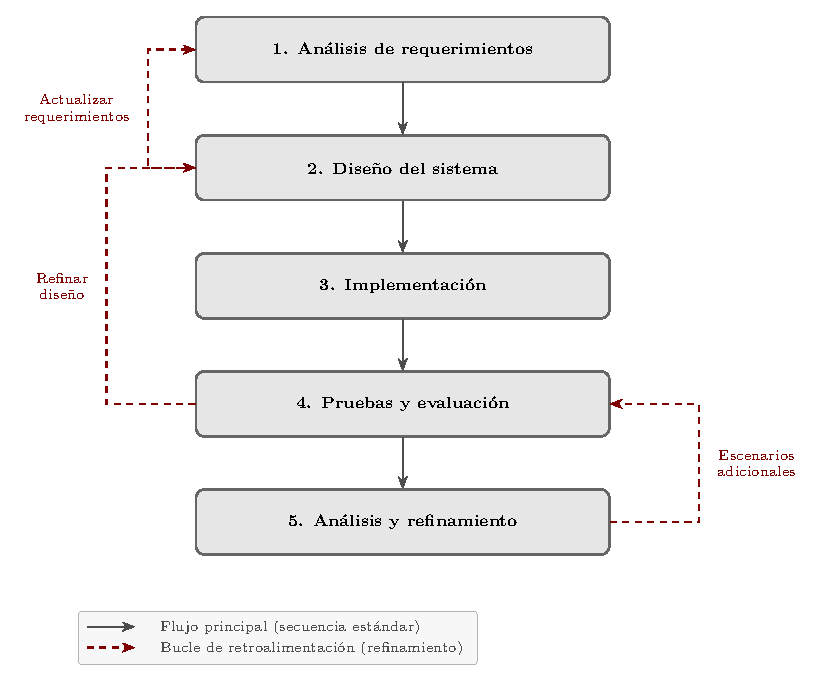
\includegraphics[width=0.80\textwidth]{figures/fig_m1_cascada.pdf}
  \caption{Modelo en cascada retroalimentada adoptado para el desarrollo del proyecto. Las flechas sólidas representan el flujo de trabajo principal; las punteadas, los caminos de retroalimentación que permiten regresar a fases anteriores cuando los resultados lo exigen.}
  \label{fig:cascada}
\end{figure}

El trabajo se organiza en seis fases: (1) \emph{requerimientos y revisión del estado del arte}, donde se definen los requerimientos del estudio y se construye el marco teórico; (2) \emph{análisis del escenario}, donde se caracterizan la geometría del enlace LEO y los parámetros NPRACH; (3) \emph{diseño del sistema}, donde se definen los bloques del modelo y las adaptaciones sobre los principios de SARA y NORA (el resto de este capítulo); (4) \emph{implementación} de los módulos en el simulador ---capa física LEO, canal, detector de colisiones, scheduler NPRACH, codebooks SCMA y decodificador MPA--- documentada en el \cref{ch:implementacion}; (5) \emph{verificación y validación} de cada módulo contra resultados publicados; y (6) \emph{análisis de resultados y conclusiones} (\cref{ch:resultados}), donde se ejecutan las campañas de simulación variando la carga de UEs y se comparan las métricas de los tres esquemas.

Los caminos de realimentación de la \cref{fig:cascada} operan así: si las métricas no cumplen los criterios de aceptación (\cref{sec:design_criterios}), se revisan parámetros del diseño (como el umbral $\Delta d_{\min}$ del agrupamiento o la política de asignación de codebooks); si durante el diseño aparece un requerimiento faltante, se actualiza el listado de requerimientos (\cref{sec:requerimientos}); y el análisis de resultados puede sugerir escenarios adicionales. Esta flexibilidad es la razón principal para escoger la cascada retroalimentada frente a una cascada estrictamente secuencial.

En cuanto a las herramientas, la implementación se realiza en NS-3 (\emph{Network Simulator 3}), un simulador de eventos discretos de código abierto ampliamente usado en la investigación de redes celulares. NS-3 incluye módulos de LTE y NB-IoT, pero su canal radio por defecto está pensado para enlaces terrestres, por lo que requiere las adaptaciones al enlace NTN-LEO descritas en el \cref{ch:implementacion}. El procesamiento posterior de las trazas ---cálculo de métricas, curvas de capacidad y análisis de la matriz de confusión--- se realiza en Python con las bibliotecas pandas, numpy y matplotlib, y el código se gestiona con Git.

\section{Requerimientos del sistema}
\label{sec:requerimientos}
\label{ch:requerimientos}

Esta sección formaliza los requerimientos del procedimiento de acceso aleatorio adaptado para redes no terrestres (NTN) con satélites LEO, expresados de manera independiente de cualquier herramienta de simulación o lenguaje de implementación. Los requerimientos se clasifican en \emph{funcionales}, que describen qué debe hacer el sistema, y \emph{no funcionales}, que describen cómo debe comportarse respecto a rendimiento, compatibilidad y robustez. Se incluyen también las restricciones de diseño impuestas por la capa física NB-IoT y por la normativa 3GPP para NTN.

El trabajo propone dos esquemas de la familia \textbf{CRACS} (\emph{Collision-detected Random Access with Codebook SCMA}): \textbf{CRACS-R} (codebook aleatorio del catálogo) y \textbf{CRACS-T} (codebook por clúster ToA). Ambos comparten el núcleo de detección probabilística de colisión, multiplexación T-SCMA en MSG3 y decodificación MPA, y difieren en la estrategia de asignación de codebook. Por ello, los requerimientos funcionales se clasifican en tres bloques: (i) \emph{compartidos} por ambos esquemas, (ii) específicos de \textbf{CRACS-R}, y (iii) específicos de \textbf{CRACS-T}. La columna \emph{Aplica} de la \cref{tab:rf} explicita esta clasificación.

\subsection{Requerimientos funcionales}
\label{sec:rf}

La \cref{tab:rf} enumera los requerimientos funcionales del sistema. Cada requerimiento se identifica con un código único \texttt{RF-XX} y su cumplimiento se verificará durante la fase de pruebas, ejecutada sobre la implementación documentada en el \cref{ch:implementacion}. Los requerimientos se expresan en términos cualitativos --qué debe hacer el sistema-- sin fijar valores numéricos; las magnitudes concretas (probabilidades del detector, número de codebooks, umbral de agrupamiento, etc.) se establecen como criterios de sistema en los requerimientos no funcionales (\cref{sec:rnf}) y en las restricciones de diseño (\cref{sec:restricciones}), y se concretan más adelante en este capítulo.

\begin{table}[H]
\centering
\caption{Requerimientos funcionales del sistema.}
\label{tab:rf}
\small
\begin{tabularx}{\textwidth}{@{}l X c c@{}}
\toprule
\textbf{ID} & \textbf{Descripción} & \textbf{Aplica} & \textbf{Prioridad} \\
\midrule
RF-01 & El sistema debe modelar la geometría tridimensional del enlace UE--satélite y la dinámica orbital, de modo que cada UE tenga asociados su distancia al satélite, su retardo de propagación y su ángulo de elevación. & Compartido & Alta \\
\addlinespace
RF-02 & El eNB debe detectar de forma probabilística las colisiones de preámbulo en el canal NPRACH. & Compartido & Alta \\
\addlinespace
RF-03 & Cada UE debe transmitir MSG3 sobre la capa SCMA asignada, adjuntando un piloto DMRS tomado del pool anunciado y su identidad de usuario. & Compartido & Alta \\
\addlinespace
RF-04 & El eNB debe decodificar las transmisiones MSG3 superpuestas mediante el decodificador MPA y clasificar cada transmisión --capa propia, capa compartida o colisión de piloto-- para resolver el acceso. & Compartido & Alta \\
\addlinespace
RF-05 & El procedimiento debe resolver de forma concurrente varias entidades (clústeres en CRACS-T o codebooks en CRACS-R) dentro de una misma ventana RACH, hasta el límite que imponga el número de codebooks SCMA disponibles. & Compartido & Media \\
\addlinespace
RF-06 & El procedimiento debe operar bajo el retardo de ida y vuelta extendido del enlace LEO sin alterar las ventanas temporales especificadas para NTN. & Compartido & Alta \\
\addlinespace
RF-07 & Los UEs que no completen el acceso en un intento deben reintentar mediante backoff aleatorio, hasta un número máximo de intentos configurable. & Compartido & Media \\
\addlinespace
RF-08 & Ante una colisión, el eNB debe emitir dos RARs con identificadores temporales distintos, cada uno anunciando el catálogo de codebooks SCMA y el pool de pilotos; cada UE colisionante debe escoger al azar una RAR, un codebook y un piloto antes de transmitir MSG3. & CRACS-R & Alta \\
\addlinespace
RF-09 & El eNB debe agrupar los UEs colisionantes en clústeres disjuntos según su distancia diferencial al satélite. & CRACS-T & Alta \\
\addlinespace
RF-10 & Por cada clúster, el eNB debe emitir una única RAR que provea un identificador temporal compartido, una capa SCMA asignada de forma determinista, la concesión de recurso uplink y la referencia de timing del clúster. & CRACS-T & Alta \\
\bottomrule
\end{tabularx}
\end{table}

\subsection{Requerimientos no funcionales}
\label{sec:rnf}

La \cref{tab:rnf} lista los requerimientos no funcionales. Se expresan como criterios cuantificables verificables contra las métricas de desempeño definidas en la \cref{sec:design_kpis}.

\begin{table}[H]
\centering
\caption{Requerimientos no funcionales del sistema.}
\label{tab:rnf}
\small
\begin{tabularx}{\textwidth}{@{}l X X@{}}
\toprule
\textbf{ID} & \textbf{Descripción} & \textbf{Criterio de aceptación} \\
\midrule
RNF-01 & La complejidad computacional del decodificador MPA debe estar acotada en número de iteraciones por ventana MSG3. & $I_{\text{MPA}} \leq 10$ iteraciones \\
\addlinespace
RNF-02 & El diseño debe ser compatible con la capa física NB-IoT NPUSCH Format~1 y operar sobre una subportadora única de 15 kHz. & Sin modificación al PHY estándar \\
\addlinespace
RNF-03 & El mecanismo de agrupamiento y resolución debe operar sin señalización adicional fuera de la cadena MSG1--MSG5. & Cero mensajes de control extra \\
\addlinespace
RNF-04 & Los parámetros del modelo deben ser trazables a especificaciones 3GPP para NTN. & Correspondencia formal con 3GPP TR~36.763 y TR~38.821 \\
\addlinespace
RNF-05 & CRACS-T debe degradar de forma controlada a comportamiento equivalente a CRACS-R (un único clúster con codebook compartido) cuando $\Delta d_{\min}$ no permite separar a los UEs colisionantes. & Fallback determinista ante proximidad extrema \\
\addlinespace
RNF-06 & El sistema debe ser reproducible: la evaluación debe entregar resultados estadísticamente consistentes. & Media e intervalo de confianza al 95\% con al menos 30 repeticiones \\
\addlinespace
RNF-07 & El detector probabilístico de colisiones debe ofrecer una fiabilidad suficiente para no degradar el acceso por detecciones omitidas o falsas alarmas. & $p_{\text{det}} \geq 0{,}975$ y $p_{\text{fa}} \leq 0{,}001$ \\
\bottomrule
\end{tabularx}
\end{table}

\subsection{Restricciones de diseño}
\label{sec:restricciones}

El diseño se acota por las siguientes restricciones, derivadas de la especificación NB-IoT y de la viabilidad del decodificador MPA:

\begin{itemize}[leftmargin=*, noitemsep]
  \item \textbf{Ancho de banda uplink.} Una sola subportadora de 15~kHz (NB-IoT NTN no permite multitono en uplink en la banda de interés).
  \item \textbf{Longitud de la ventana T-SCMA.} Máximo $N = 4$ subframes por ventana, alineado con la estructura de dos slots de NPUSCH Format~1.
  \item \textbf{Número de codebooks SCMA.} Máximo $K_{\text{CB}} = 6$, con sobreocupación $K_{\text{CB}}/N = 150\%$, límite práctico de separabilidad del receptor MPA.
  \item \textbf{Ángulo de elevación mínimo.} $\alpha_{\min}$ configurable en el rango $10^\circ$--$30^\circ$, con el compromiso entre cobertura angular y pérdida de enlace.
  \item \textbf{Distancia diferencial mínima.} $\Delta d_{\min} = 150$~m, correspondiente a la resolución temporal del NPRACH a 15~kHz de subportadora.
  \item \textbf{Número de pilotos DMRS ortogonales.} 3 por capa SCMA, máximo teórico de cyclic shifts ortogonales compatibles con $N = 4$ recursos.
  \item \textbf{Preámbulos disponibles.} $N_{\text{pream}} = 48$, conforme a la especificación NB-IoT para RACH.
\end{itemize}

Estas restricciones se asumen fijas durante el diseño y solo se revisan si la fase de evaluación demuestra que su violación es necesaria para alcanzar los objetivos del trabajo.

\section{Modelo de sistema NTN--LEO}
\label{sec:modelo_sistema}

El escenario de estudio consiste en un único satélite LEO en órbita circular que actúa como eNB para una población de terminales NB-IoT estacionarios desplegados sobre una huella terrestre rural. La \cref{fig:system_model} es la representación de referencia del sistema y consolida los elementos geométricos, el modelo de cobertura y los supuestos de canal sobre los que se construye el resto del capítulo. En ella, la geometría queda definida por la altitud orbital $h_{\text{sat}}$, el slant range $d_{\text{slant}}$ entre cada UE y el satélite, el ángulo de elevación local $\alpha$ y el ángulo de elevación mínimo $\alpha_{\min}$ que delimita la cobertura; los UEs se distribuyen uniformemente en un disco de radio $R_{\text{cell}}$ centrado en el punto sub-satelital, y los terminales con elevación inferior a $\alpha_{\min}$ se consideran fuera de servicio.

\begin{figure}[H]
  \centering
  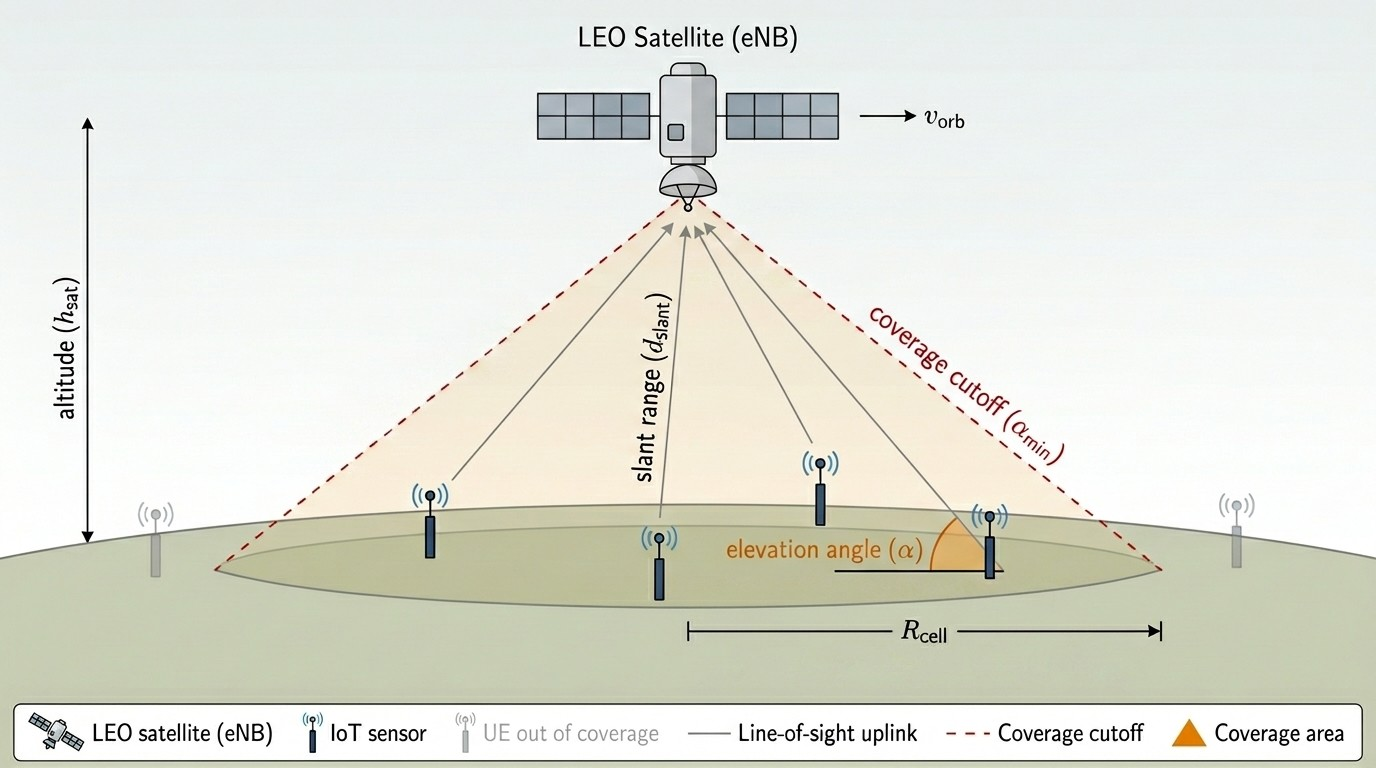
\includegraphics[width=0.95\textwidth]{esquema_general.jpg}
  \caption{Modelo de sistema NB-IoT sobre un único satélite LEO.}
  \label{fig:system_model}
\end{figure}

Los parámetros numéricos del modelo de referencia se listan en la \cref{tab:parametros}.\footnote{El \emph{nadir} es el punto de la superficie terrestre situado directamente bajo el satélite; el RTT mínimo se da cuando el UE coincide con el nadir y el slant range se reduce a la altitud orbital $h_{\text{sat}}$.}

\begin{table}[H]
\centering
\caption{Parámetros del modelo de sistema.}
\label{tab:parametros}
\small
\begin{tabular}{@{}l c l l@{}}
\toprule
\textbf{Parámetro} & \textbf{Símbolo} & \textbf{Valor de referencia} & \textbf{Fuente} \\
\midrule
Altitud orbital & $h_{\text{sat}}$ & 600 km & 3GPP TR 36.763 \\
Velocidad orbital & $v_{\text{sat}}$ & $\sim$7.5 km/s & Mecánica orbital LEO \\
Ángulo de elevación mínimo & $\alpha_{\min}$ & $10^\circ$--$45^\circ$ (default $40^\circ$) & Configurable \\
RTT mínimo (nadir) & $\mathrm{RTT}_{\min}$ & $\sim$4 ms & Cálculo \\
RTT máximo (borde de cobertura) & $\mathrm{RTT}_{\max}$ & $\sim$27 ms & $\alpha_{\min}=10^\circ$ \\
Pérdida atmosférica & $L_{\text{atm}}$ & $0{,}53$ dB (constante) & Modelo de referencia \\
FSPL promedio & $L_{\text{FSPL}}$ & $150$ dB (constante) & Modelo de referencia \\
Margen de enlace & $L_{\text{margin}}$ & $0{,}82$ dB (constante) & Reserva de diseño \\
Ganancia de antena UE & $G_{\text{UE}}$ & isotrópica & Modelo de referencia \\
\bottomrule
\end{tabular}
\end{table}

La potencia recibida por cada UE activo dentro del cono de cobertura se modela como
\begin{equation}
  P_{\text{RX}} = P_{\text{TX}} - L_{\text{atm}} - L_{\text{FSPL}} - L_{\text{margin}}.
  \label{eq:link_budget}
\end{equation}
Las tres pérdidas se toman constantes; los valores concretos empleados en la evaluación se listan en la \cref{tab:impl_flags}. Los UEs cuya elevación sea inferior a $\alpha_{\min}$ se consideran fuera de servicio mediante un criterio binario (dentro o fuera de cobertura).

\paragraph{Aspectos modelados.} El sistema considera la geometría tridimensional del enlace UE--satélite a partir de las coordenadas ECEF, incluyendo la dinámica orbital del satélite a lo largo del tiempo, el RTT por UE calculado como $2 d_{\text{slant}}/c$, el criterio de cobertura por elevación mínima ($\alpha_{\min}$), que clasifica a cada UE como dentro o fuera de servicio, un balance de enlace con pérdidas atmosféricas y de espacio libre constantes y un margen fijo, y la distancia diferencial $\Delta d = d_{\text{slant}} - h_{\text{sat}}$, magnitud geométrica cuyo papel en el agrupamiento se detalla más adelante en la \cref{sec:cracs_t}.

\paragraph{Aspectos no modelados.} Para concentrar el análisis en el procedimiento de acceso, el modelo asume condiciones ideales de canal y no representa: la variación de FSPL con la distancia ($1/r^2$), el desvanecimiento rápido (Rician o Rayleigh), el sombreado log-normal, el desplazamiento Doppler debido al movimiento del satélite, la atenuación por lluvia y el centelleo ionosférico, el patrón de radiación de las antenas (se asume ganancia isotrópica) y la dispersión por multitrayecto. Estos aspectos se asumen bajo condiciones ideales de canal para concentrar el análisis en el desempeño del procedimiento de acceso; declararlos de forma explícita acota el alcance de validez de los resultados de capacidad.

\paragraph{Asunción de propagación en línea de vista.} El modelo asume canal de propagación en línea de vista entre cada UE en cobertura y el satélite, con pérdidas constantes ($L_{\text{atm}}$, $L_{\text{FSPL}}$, $L_{\text{margin}}$) y un criterio de cobertura de tipo todo-o-nada (el UE está dentro o fuera de servicio) según el ángulo de elevación mínimo. Esta abstracción es consistente con el nivel de detalle propio de un análisis de acceso aleatorio a nivel de sistema, donde el foco no es la caracterización fina del enlace sino el desempeño agregado del procedimiento de acceso bajo carga creciente. Los efectos de propagación más realistas identificados en los \emph{Aspectos no modelados} se reservan como extensiones de trabajo futuro.

\section{Visión general de los esquemas evaluados}
\label{sec:vision}

Este trabajo propone dos esquemas que conforman la familia \textbf{CRACS} (\emph{Collision-detected Random Access with Codebook SCMA}): \textbf{CRACS-R} (codebook aleatorio del catálogo) y \textbf{CRACS-T} (codebook por clúster ToA). Ambos comparten un núcleo común sobre la cadena estándar de acceso aleatorio NB-IoT: (i) un \emph{detector probabilístico de colisiones} de preámbulo en el eNB, (ii) una \emph{multiplexación T-SCMA} del payload MSG3 que permite la resolución simultánea de múltiples UEs mediante decodificación MPA, y (iii) la \emph{individualización por IMSI} en MSG4 cuando varios UEs comparten TC-RNTI. La diferencia entre los dos esquemas radica en la \emph{estrategia de asignación de codebook} SCMA tras detectar una colisión.

\textbf{CRACS-R} adapta el principio de SARA (Moon et al., 2021) al contexto NB-IoT NTN incorporando SCMA: tras detectar colisión, el eNB emite dos RARs anunciando el catálogo completo de codebooks; cada UE elige aleatoriamente un codebook y un piloto DMRS. Es un esquema sin información geométrica adicional, dependiente del azar y de la separación posterior por MPA.

\textbf{CRACS-T} extiende el principio NORA (Wang et al., 2020) incorporando un agrupamiento espacial de los UEs colisionantes basado en su distancia diferencial al satélite, y \emph{asignación determinista} del codebook SCMA por clúster: tras detectar colisión, el eNB analiza los tiempos de llegada de los preámbulos superpuestos, los agrupa en clústeres espaciales y emite una RAR por clúster con TC-RNTI compartido y codebook fijo asignado. Aprovecha la geometría LEO para reducir la contienda residual aguas abajo.

La \cref{tab:esquemas} contrasta los tres esquemas considerados en este trabajo: el baseline Legacy y las dos propuestas CRACS-R y CRACS-T.

\begin{table}[H]
\centering
\caption{Comparación de los tres esquemas considerados.}
\label{tab:esquemas}
\small
\begin{tabularx}{\textwidth}{@{}l X X X@{}}
\toprule
\textbf{Aspecto} & \textbf{Legacy (baseline)} & \textbf{CRACS-R (propuesta 1)} & \textbf{CRACS-T (propuesta 2)} \\
\midrule
Detección de colisión MSG1 & No & Probabilística & Probabilística \\
Agrupamiento espacial & No aplica & No aplica & Sí, por $\Delta d$ \\
RARs emitidos por colisión & 1 (no distingue) & 2 (fijo por diseño) & 1 por clúster \\
Asignación de codebook & No aplica & Catálogo anunciado, sorteo por UE & Determinista por clúster \\
Pilotos DMRS & Únicos por UE & Pool anunciado, sorteo por UE & Pool compartido, sorteo por UE \\
Resolución MSG3 & Ninguna (fallo por superposición) & MPA tras sorteo aleatorio & MPA con contexto de clúster \\
Colisión de pilotos & No aplica & Posible (diseño) & Minimizada (por clustering) \\
Individualización de C-RNTI & TC-RNTI único & Por TC-RNTI distinto o IMSI & Por IMSI en RRC \\
\bottomrule
\end{tabularx}
\end{table}

\section{Arquitectura general del proceso de simulación}
\label{sec:arquitectura}

La \cref{fig:system_arch} resume el flujo general del proceso de simulación que articula los tres esquemas: a partir de los parámetros de entrada se configura el sistema y se construye el escenario; el flujo se bifurca según el esquema de acceso seleccionado (Legacy, CRACS-R o CRACS-T), y finaliza en una etapa común de evaluación de la capacidad del canal.

\begin{figure}[H]
  \centering
  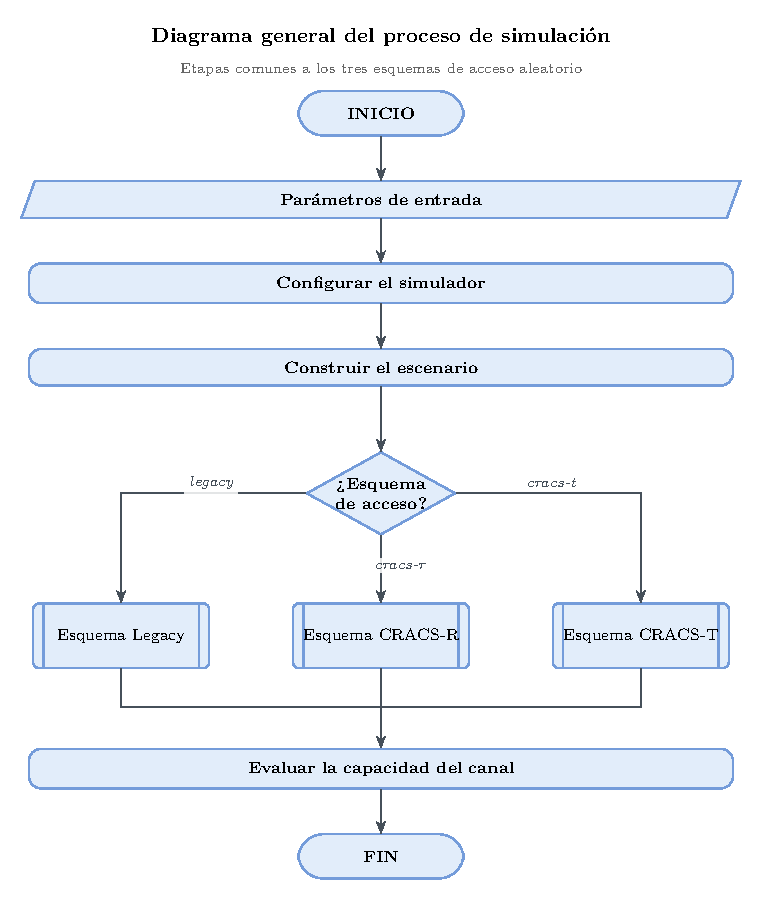
\includegraphics[width=0.95\textwidth]{fig_m3_system_arch.pdf}
  \caption{Diagrama general del proceso de simulación común a los tres esquemas.}
  \label{fig:system_arch}
\end{figure}

En detalle, cada etapa del diagrama comprende lo siguiente. La etapa de \emph{parámetros de entrada} fija el esquema de acceso bajo prueba (Legacy, CRACS-R o CRACS-T), la semilla de simulación, el perfil de tráfico, la geometría orbital LEO ($h_{\text{sat}}$, $\alpha_{\min}$ y posición central), el modelo de canal y los parámetros del detector probabilístico de colisión (en CRACS-R y CRACS-T). La etapa \emph{configurar el simulador} activa el esquema seleccionado y establece los parámetros del canal LEO y de la temporización NTN. La etapa \emph{construir el escenario} instancia el satélite y los UEs, los distribuye sobre el área de cobertura y genera los tiempos de intento de acceso. Tras ejecutar el esquema seleccionado en la bifurcación, la etapa común \emph{evaluar la capacidad del canal} recopila las métricas registradas durante la simulación y calcula los indicadores de capacidad definidos en la \cref{sec:design_kpis}.

\section{Procedimiento baseline: Legacy}
\label{sec:legacy}

El procedimiento Legacy implementa el acceso aleatorio NB-IoT estándar en cinco mensajes, cada uno con un propósito definido dentro del establecimiento de la conexión: en MSG1 el UE transmite un preámbulo aleatorio (uno entre $N_{\text{pream}} = 48$) para anunciar su intención de acceso y permitir que el eNB estime su retardo de propagación; con MSG2 (RAR) el eNB acusa el preámbulo y entrega los recursos iniciales ---TC-RNTI, \textit{timing advance} y concesión uplink--- que el UE necesita para transmitir de forma sincronizada; en MSG3 (RRC Connection Request) el UE se identifica y solicita formalmente el establecimiento de la conexión; con MSG4 (RRC Connection Setup) el eNB resuelve la contienda y asigna el identificador definitivo (C-RNTI); y MSG5 (RRC Setup Complete) cierra el procedimiento confirmando que la conexión quedó establecida. La \cref{fig:legacy} ilustra el flujo de éxito (a) y el escenario de colisión (b).

\begin{figure}[H]
  \centering
  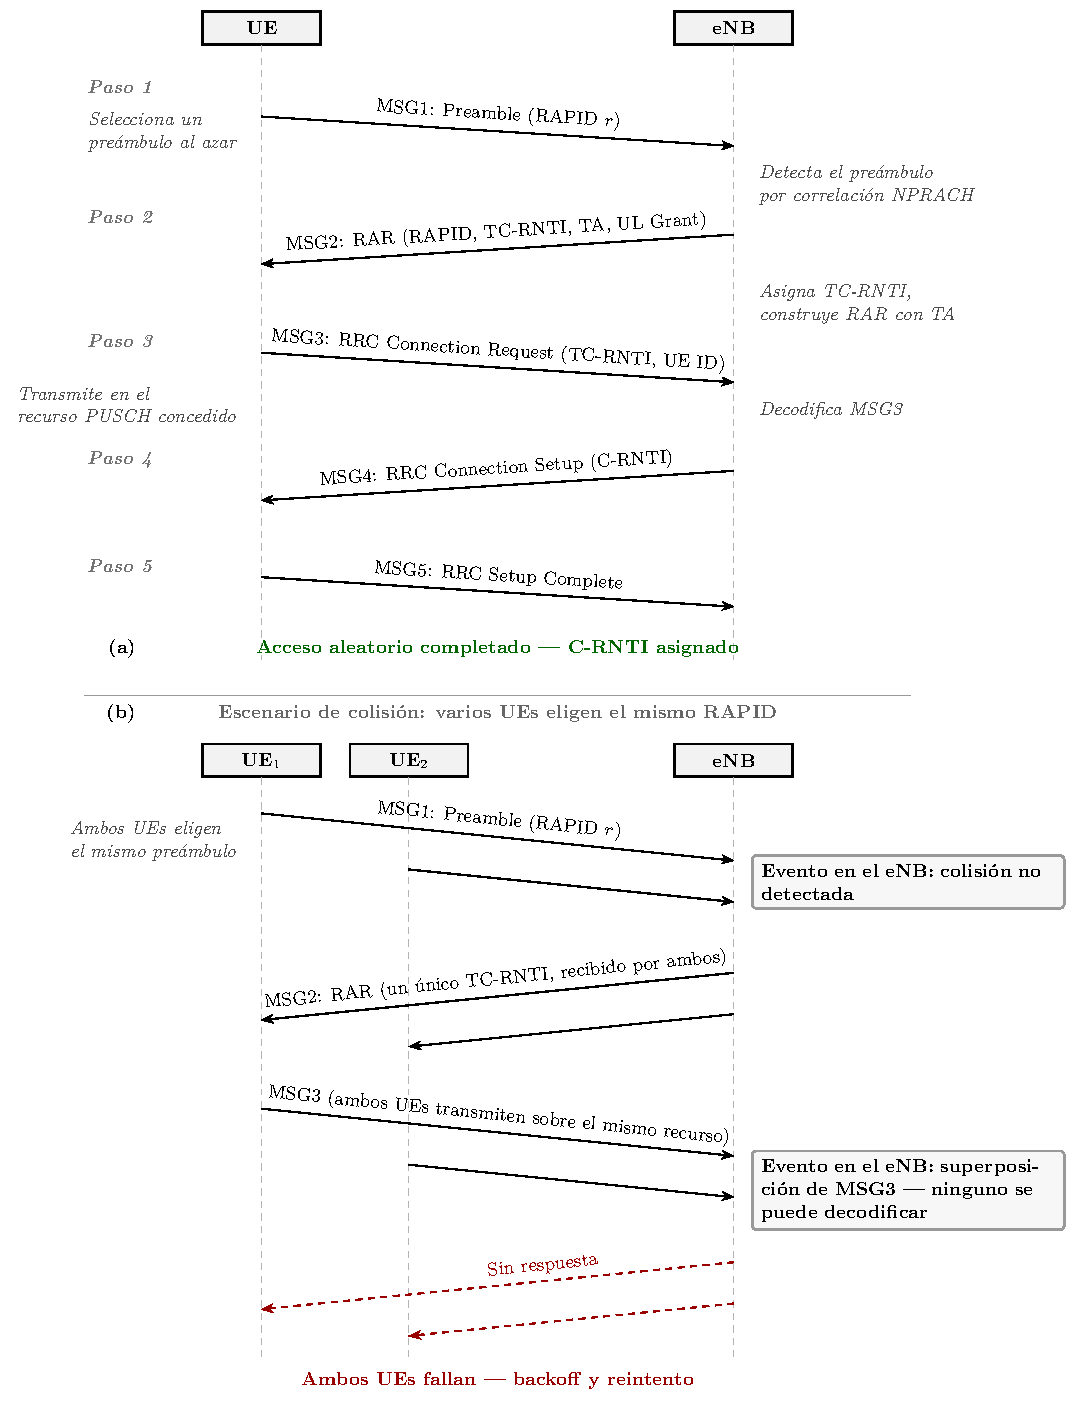
\includegraphics[width=0.95\textwidth]{fig2_legacy_msc.pdf}
  \caption{Procedimiento de acceso aleatorio baseline (Legacy): flujo de éxito y escenario de colisión.}
  \label{fig:legacy}
\end{figure}

En la \cref{fig:legacy} las etiquetas se presentan en forma genérica: solo se identifican los mensajes intercambiados (MSG1--MSG5 con sus campos: RAPID, TC-RNTI, TA, UL Grant, C-RNTI) y la tarea ejecutada a cada lado (selección de preámbulo en el UE; detección, asignación de TC-RNTI, construcción de la RAR y decodificación de MSG3 en el eNB). El tamaño del pool de preámbulos disponibles ($N_{\text{pream}} = 48$) y el resto de parámetros numéricos se enuncian en el párrafo previo.

En el escenario de colisión, el eNB observa un único pico de correlación NPRACH para el RAPID colisionado y emite una sola RAR con un único TC-RNTI. Los UEs colisionantes reciben idéntica RAR y responden con MSG3 sobre el mismo recurso PUSCH. La superposición de las transmisiones impide la decodificación: el eNB no recibe ningún MSG3 válido y la ventana de contienda expira. Los UEs retransmiten el preámbulo tras un backoff aleatorio.

\section{Primera propuesta: CRACS-R (codebook aleatorio del catálogo)}
\label{sec:cracs_r}

\textbf{CRACS-R} es la primera propuesta de la familia CRACS. Adapta el principio de SARA (Moon et al., 2021) al contexto NB-IoT NTN incorporando SCMA en MSG3 y detección probabilística de colisión en el eNB. Es un esquema deliberadamente \emph{sin información geométrica}: la separación de UEs colisionantes se delega íntegramente al sorteo aleatorio de codebooks y pilotos seguido de decodificación MPA. La \cref{fig:sara} ilustra el flujo con tres UEs colisionantes.

\begin{figure}[H]
  \centering
  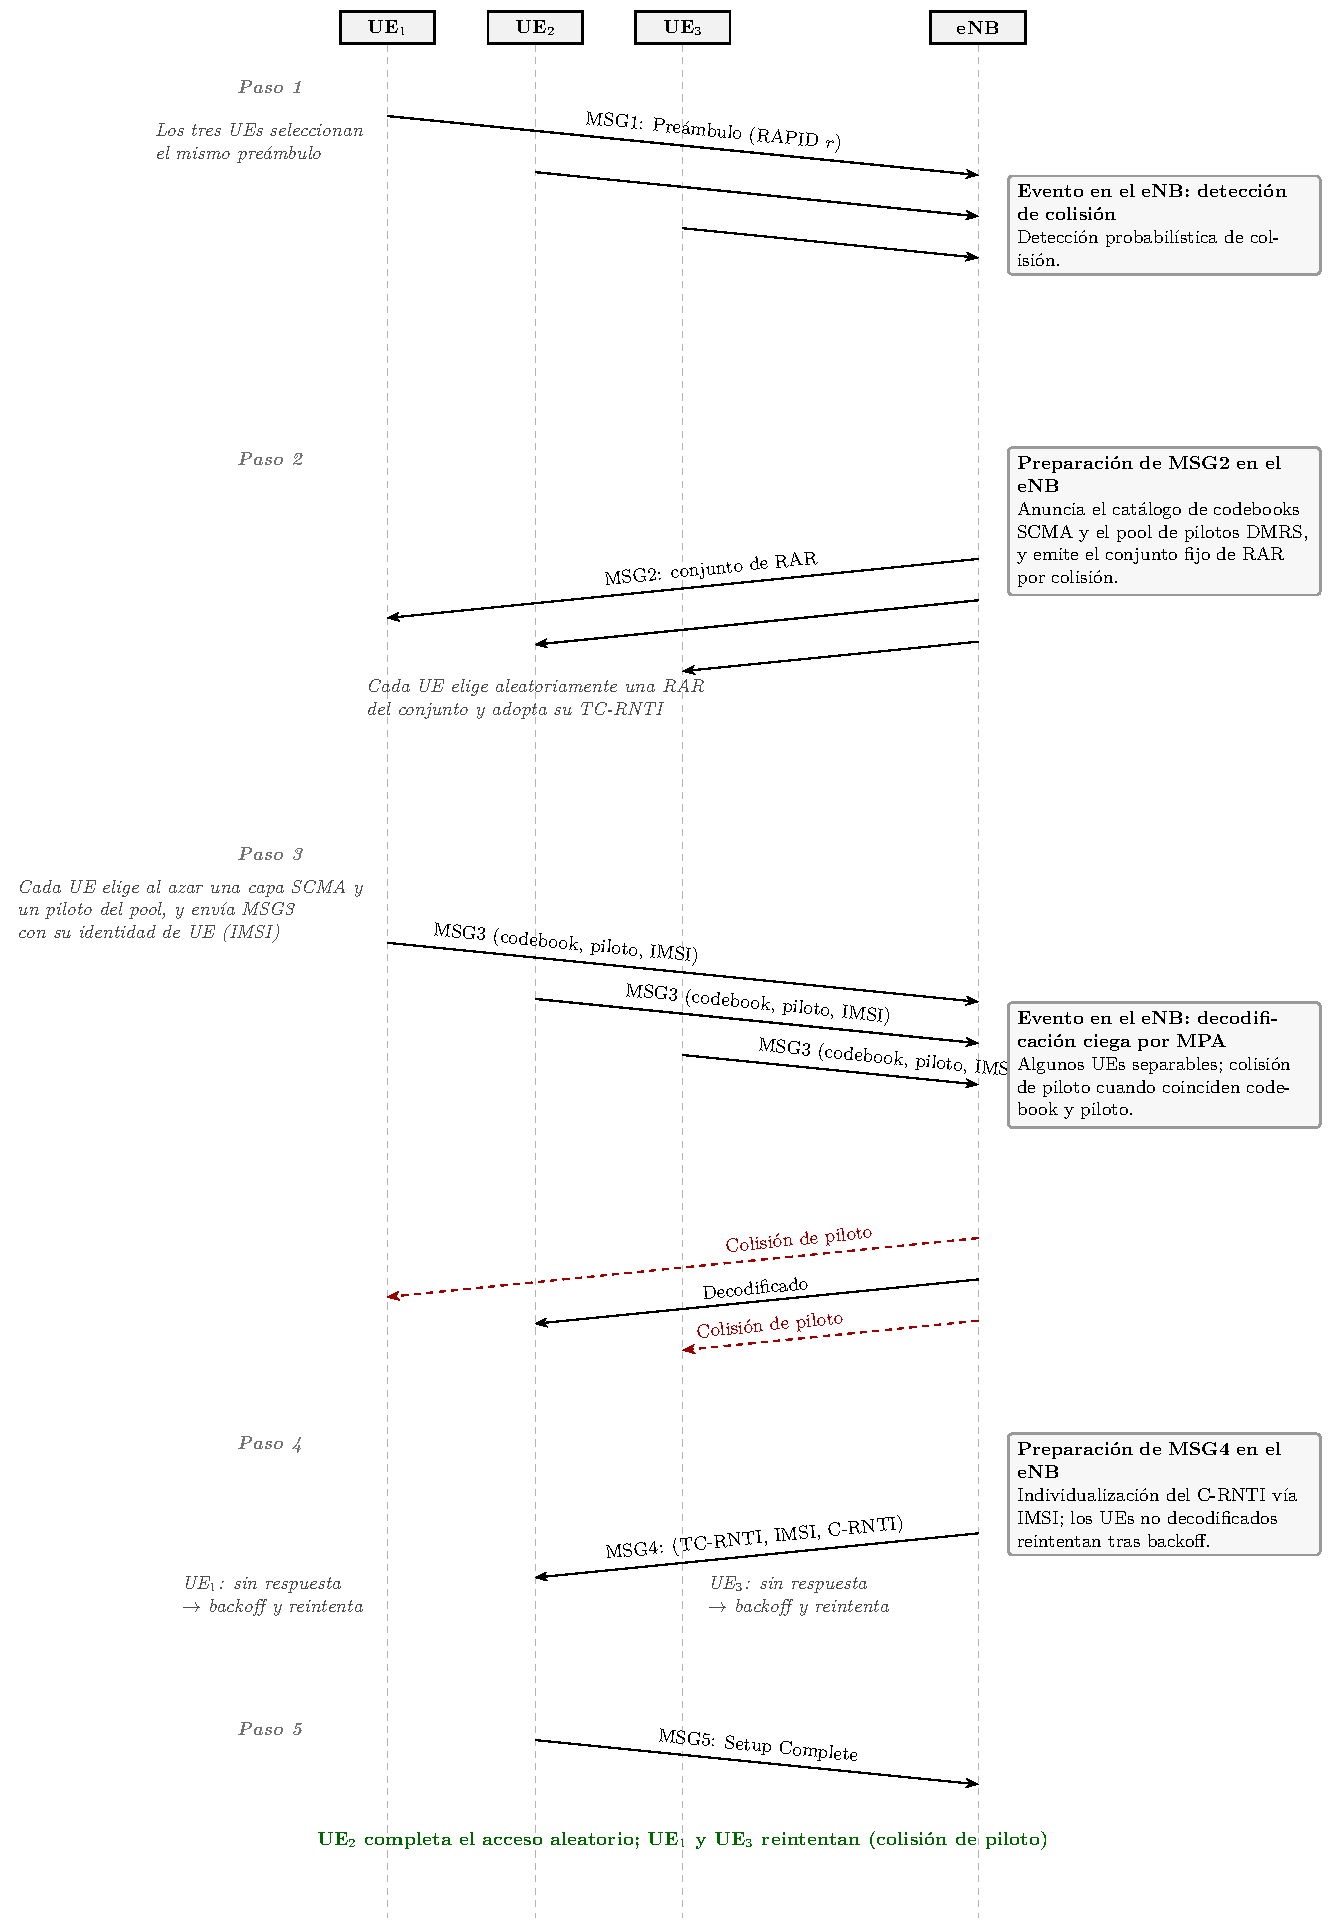
\includegraphics[width=0.95\textwidth]{fig3_sara_msc.pdf}
  \caption{Procedimiento CRACS-R con tres UEs colisionantes.}
  \label{fig:sara}
\end{figure}

En la \cref{fig:sara} las etiquetas se presentan en forma genérica (sin valores ni índices específicos): solo se identifican los mensajes y las tareas. Las probabilidades del detector ($p_{\text{det}}=0{,}975$, $p_{\text{fa}}=0{,}001$), el tamaño del catálogo de codebooks SCMA ($K_{\text{CB}}=6$), la cardinalidad del pool de pilotos DMRS ($D=3$) y la cantidad fija de RARs emitidos por colisión (\emph{dos}) se enuncian en los ítems del listado que sigue.

Los puntos clave del diseño de CRACS-R son:
\begin{itemize}[leftmargin=*, noitemsep]
  \item \textbf{Detección probabilística}: el eNB dispone de un detector con probabilidad $p_{\text{det}} = 0.975$ y $p_{\text{fa}} = 0.001$; sin embargo, solo conoce \emph{que} ocurrió una colisión, no cuántos UEs están involucrados.
  \item \textbf{Dos RARs fijos}: dado que el mínimo para que exista colisión es de dos UEs, el eNB emite siempre dos RARs, cada uno con un TC-RNTI distinto y con el catálogo completo de capas SCMA ($K = 6$) y de pilotos DMRS ($D = 3$).
  \item \textbf{Elección aleatoria del UE}: cada UE selecciona una RAR al azar (lo que implica que dos UEs pueden terminar compartiendo TC-RNTI) y, en MSG3, una capa SCMA y un piloto DMRS al azar del pool anunciado.
  \item \textbf{Resolución por MPA}: el eNB decodifica las transmisiones MSG3 superpuestas mediante MPA. Si dos UEs eligieron la misma capa y el mismo piloto (colisión de piloto), ambos fallan; en otros casos, el eNB puede separarlos.
  \item \textbf{Individualización en RRC}: cuando los UEs comparten TC-RNTI, la individualización del C-RNTI se realiza en MSG4 usando el IMSI transmitido en el RRC Connection Request.
\end{itemize}

\section{Segunda propuesta: CRACS-T (codebook por clúster ToA)}
\label{sec:cracs_t}

\textbf{CRACS-T} es la segunda propuesta de la familia CRACS. Extiende el principio NB-NORA introducido por Wang \emph{et al.} (2020) incorporando agrupamiento espacial de los UEs colisionantes basado en su distancia diferencial al satélite y \emph{asignación determinista} del codebook SCMA por clúster. Aprovecha la dispersión de tiempos de llegada característica del enlace LEO para particionar los UEs colisionantes \emph{antes} de emitir las RARs, reduciendo la contienda residual aguas abajo. La \cref{fig:new} ilustra el flujo completo con tres UEs que caen en un mismo clúster.

\begin{figure}[H]
  \centering
  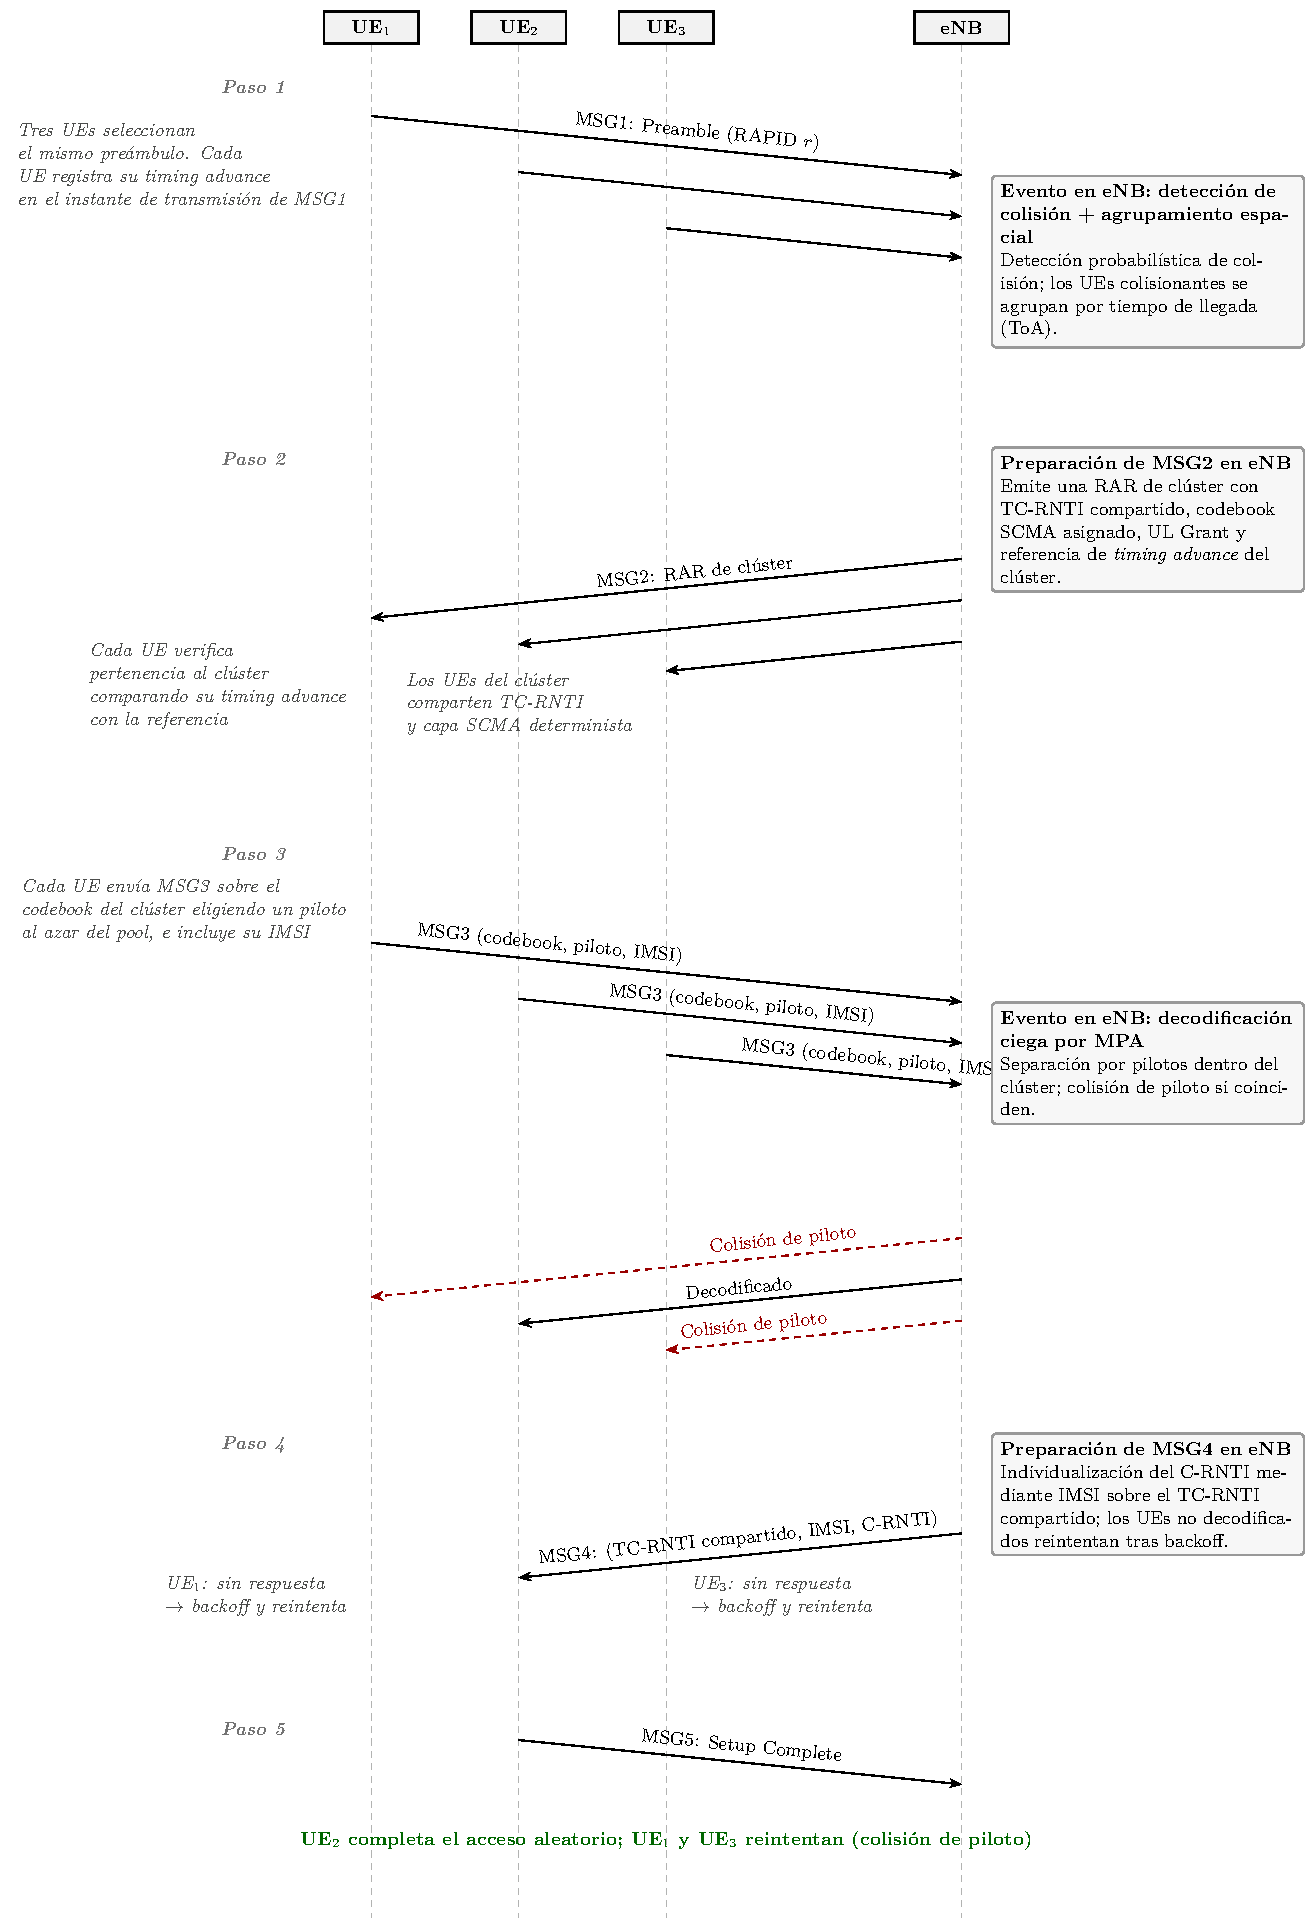
\includegraphics[width=0.95\textwidth]{fig4_new_msc.pdf}
  \caption{Procedimiento de acceso aleatorio de CRACS-T con tres UEs colisionantes agrupados en un mismo clúster.}
  \label{fig:new}
\end{figure}

En la \cref{fig:new} las etiquetas se presentan en forma genérica: solo se identifican los mensajes intercambiados, los pasos del procedimiento y las tareas ejecutadas a cada lado (detección probabilística + agrupamiento por ToA en el eNB; verificación de pertenencia al clúster en el UE; decodificación MPA e individualización por IMSI). Las probabilidades del detector ($p_{\text{det}}=0{,}975$, $p_{\text{fa}}=0{,}001$), el umbral de separación $\Delta d_{\min}=150$~m, el tamaño del catálogo de codebooks ($K_{\text{CB}}=6$) y el pool de pilotos DMRS ($D=3$) se detallan en los pasos del flujo descritos a continuación.

El flujo se descompone en los cinco pasos siguientes:

\subsection*{Paso 1: Transmisión de preámbulo y registro de timing}
Cada UE selecciona un preámbulo al azar y lo transmite en MSG1. En el instante de transmisión, el UE registra su \emph{timing advance} actual, calculado como la distancia diferencial $\Delta d = d_{\text{slant}} - h_{\text{sat}}$. Este valor se almacena localmente y se usará en el paso 2 para confirmar la pertenencia al clúster anunciado por el eNB. El eNB, al recibir MSG1, ejecuta el detector probabilístico de colisiones.

\subsection*{Paso 2: Agrupamiento y emisión de RAR de clúster}
Si se detecta colisión en un RAPID, el eNB ordena los tiempos de llegada de los preámbulos superpuestos y realiza un barrido de clustering: dos preámbulos pertenecen al mismo clúster si su separación en $\Delta d$ es inferior a $\Delta d_{\min}$. El número de clústeres resultantes está acotado por $K_{\text{CB}}$. Por cada clúster, el eNB emite una única RAR que contiene (i) un TC-RNTI compartido, (ii) una capa SCMA determinista asignada al clúster, (iii) la concesión uplink, y (iv) el valor de $\Delta d$ representativo del clúster.

Al recibir la RAR, cada UE compara el valor $\Delta d$ recibido con el que registró al transmitir MSG1. Si la diferencia es menor que $\Delta d_{\min}/2$, el UE adopta la RAR como propia.

\subsection*{Paso 3: Transmisión MSG3 multiplexada}
Todos los UEs del mismo clúster transmiten MSG3 sobre la misma capa SCMA asignada, usando un piloto DMRS seleccionado aleatoriamente del pool ortogonal (3 pilotos disponibles). El payload incluye el IMSI del UE (necesario para la individualización en RRC). Las transmisiones se superponen sobre los $N = 4$ subframes de la ventana T-SCMA.

\subsection*{Paso 4: Resolución MPA y emisión de MSG4}
El eNB recibe la señal superpuesta y ejecuta el algoritmo MPA sobre el grafo de factores $\mathbf{F}_{4\times 6}$ (cuya estructura y propósito ---separar las transmisiones SCMA superpuestas explotando la esparsidad del codebook--- se detallan en la \cref{sec:scma}). Por cada UE cuya transmisión sea decodificable, el eNB extrae el IMSI del payload y asigna un C-RNTI individual. MSG4 se envía sobre el TC-RNTI compartido pero contiene el IMSI y el C-RNTI específicos por UE, permitiendo que cada UE identifique su propia respuesta.

\subsection*{Paso 5: Confirmación}
Cada UE decodifica MSG4, identifica su IMSI en el payload, adopta el C-RNTI asignado y confirma con MSG5 (RRC Setup Complete). Los UEs que no recibieron respuesta (por colisión de piloto o fallo de MPA) entran en backoff y reintentan desde el paso 1.

\section{Mecanismo de agrupamiento por tiempo de llegada (CRACS-T)}
\label{sec:toa}

El agrupamiento por tiempo de llegada es el rasgo distintivo de \textbf{CRACS-T} respecto a CRACS-R: es lo que le permite asignar codebooks SCMA de forma determinista en lugar de aleatoria. La \cref{fig:toa} ilustra cómo se particionan los UEs colisionantes en clústeres disjuntos según su distancia diferencial al satélite.

\begin{figure}[H]
  \centering
  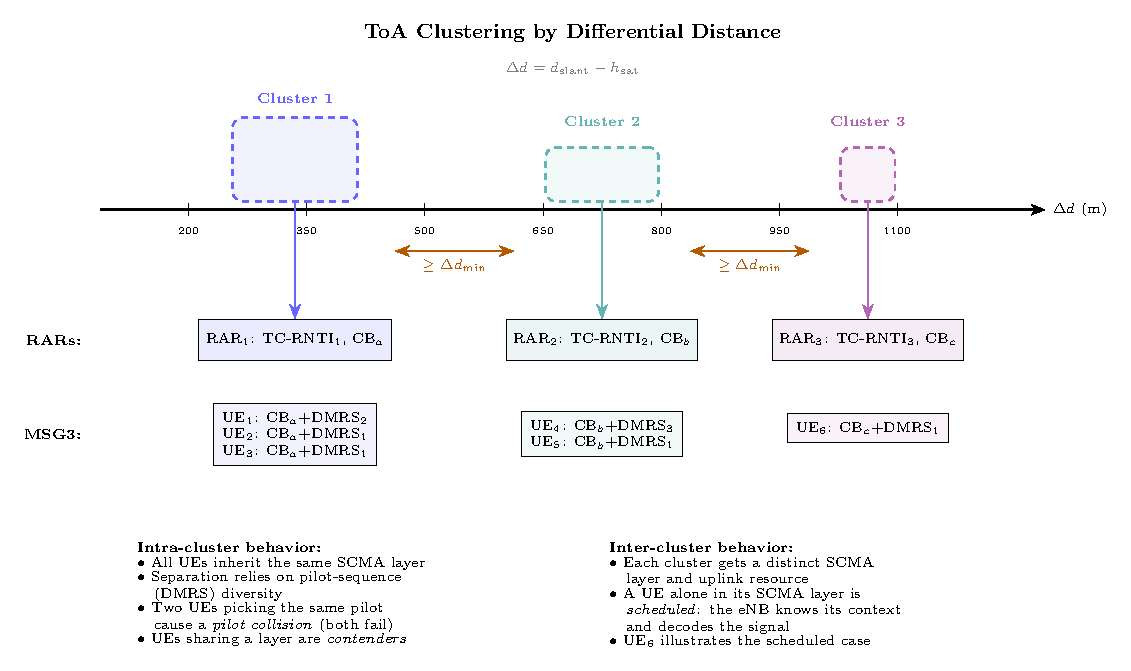
\includegraphics[width=0.95\textwidth]{fig5_toa_clustering.pdf}
  \caption{Mecanismo de agrupamiento por distancia diferencial $\Delta d$. Los UEs colisionantes se ordenan por su $\Delta d$ y se agrupan en clústeres separados por al menos $\Delta d_{\min} = 150$~m. Cada clúster recibe una RAR con TC-RNTI compartido y una capa SCMA asignada de forma determinista.}
  \label{fig:toa}
\end{figure}

Las decisiones de diseño clave son:
\begin{description}[leftmargin=1.5em,style=nextline]
  \item[Por qué $\Delta d$ y no $d_{\text{slant}}$:] la resta $d_{\text{slant}} - h_{\text{sat}}$ elimina el sesgo común dado por la altitud orbital, dejando la métrica invariante respecto a la posición instantánea del satélite. Esto hace el agrupamiento robusto frente a la deriva orbital entre MSG1 y MSG2.
  \item[Por qué $\Delta d_{\min} = 150$~m:] este valor corresponde a la resolución temporal efectiva del NPRACH con subportadora de 15~kHz. UEs más cercanos que este umbral no son separables por timing y deben tratarse como un único clúster (fallback a comportamiento CRACS-R dentro del clúster).
  \item[Algoritmo de agrupamiento:] se ordenan los valores $\Delta d$ observados en orden ascendente y se realiza un barrido lineal que abre un nuevo clúster cada vez que la separación con el anterior supera $\Delta d_{\min}$. La complejidad es $O(K \log K)$ en el número $K$ de UEs colisionantes.
  \item[Salida:] una partición $\{C_1, C_2, \ldots, C_M\}$ de los UEs colisionantes en $M$ clústeres disjuntos, con $M \leq K_{\text{CB}} = 6$.
\end{description}

\section{SCMA y grafo de factores}
\label{sec:scma}

La multiplexación SCMA empleada en MSG3 se apoya en un grafo de factores bipartito $\mathbf{F}_{N \times K}$ con $N = 4$ recursos (subframes) y $K = 6$ codebooks. La \cref{fig:factor_graph} presenta la estructura del grafo y la matriz indicadora que lo codifica.

\begin{figure}[H]
  \centering
  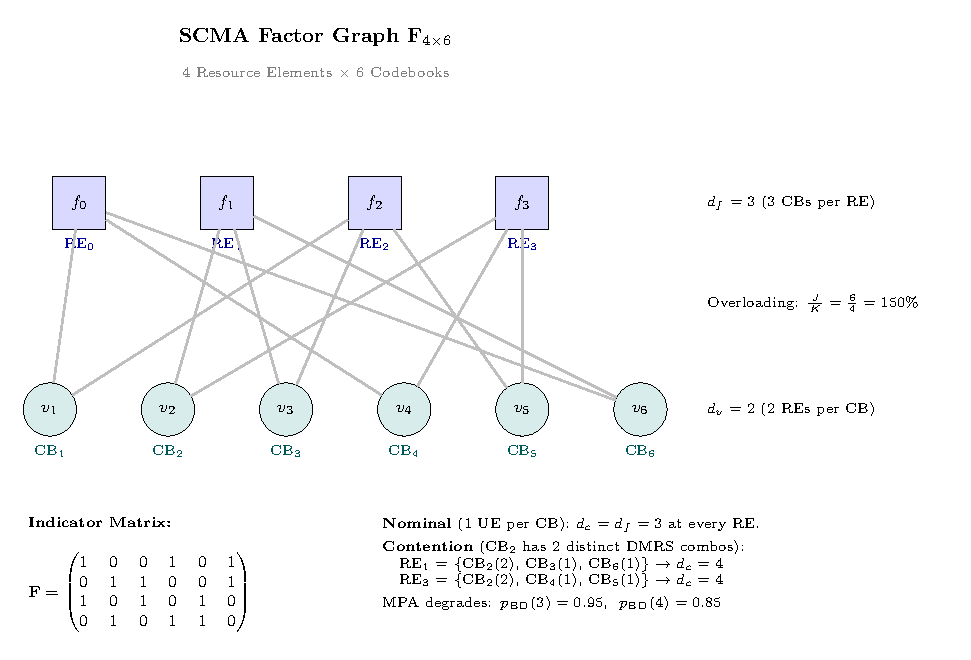
\includegraphics[width=0.85\textwidth]{fig6_factor_graph.pdf}
  \caption{Grafo de factores SCMA $\mathbf{F}_{4 \times 6}$. Los nodos de función (rectángulos) representan los cuatro elementos de recurso; los nodos de variable (círculos) representan los seis codebooks. Cada codebook ocupa $d_v = 2$ recursos y cada recurso acomoda $d_f = 3$ codebooks, con una sobreocupación $K/N = 150\%$.}
  \label{fig:factor_graph}
\end{figure}

Las propiedades del grafo relevantes al diseño son: el grado de cada nodo de función $d_f = 3$ determina cuántos codebooks se superponen en un mismo recurso; el grado de cada nodo de variable $d_v = 2$ determina cuántos recursos utiliza cada codebook (esparsidad temporal); el número total de codebooks es $K = \binom{N}{d_v} = \binom{4}{2} = 6$, lo que agota el espacio combinatorio y garantiza que cada codebook ocupe un patrón distinto.

\section{Diseño T-SCMA para el uplink MSG3}
\label{sec:tscma}

La multiplexación SCMA se implementa en el dominio del tiempo siguiendo la técnica T-SCMA propuesta por Yan \emph{et al.} (2017) específicamente para NB-IoT, ya que el ancho de banda de una subportadora de 15~kHz no admite multiplexación clásica en frecuencia. Apoyándose en el grafo de factores de la \cref{fig:factor_graph}, la \cref{fig:tscma_multiplex} ilustra cómo se organiza la transmisión paralela de $K = 6$ codebooks sobre $N = 4$ subframes en una única subportadora de 15~kHz, mientras que la \cref{fig:tscma_symbol} detalla la estructura de símbolo dentro de un subframe activo.

\begin{figure}[H]
  \centering
  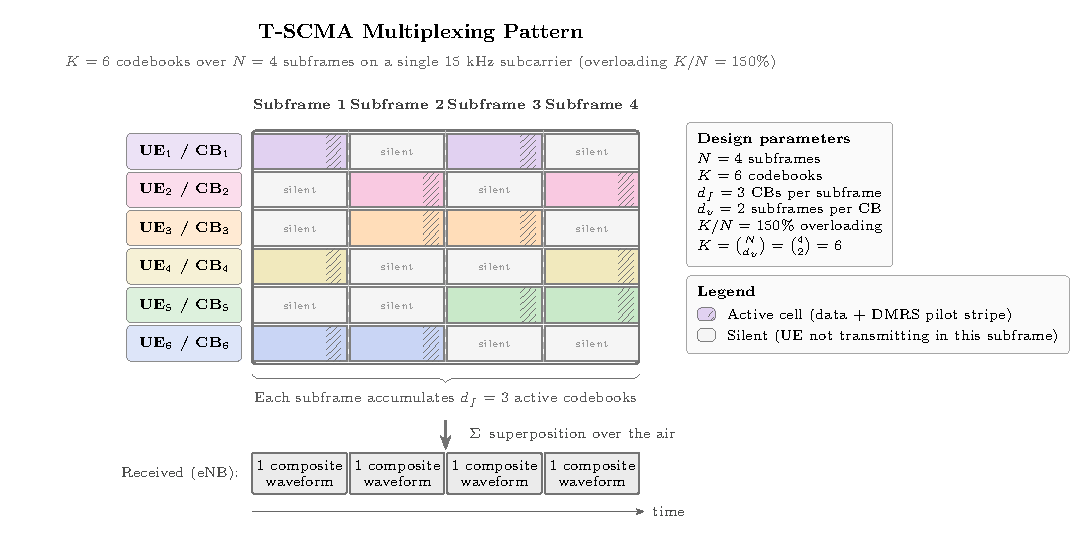
\includegraphics[width=0.95\textwidth]{fig8_tscma_design.pdf}
  \caption{Patrón de multiplexación T-SCMA. La cuadrícula muestra los seis UEs (filas) y los cuatro subframes (columnas). Cada celda activa indica que el UE transmite en ese subframe (datos más piloto DMRS); las celdas \emph{silent} indican subframes en los que el UE no transmite. En cada subframe se acumulan hasta $d_f = 3$ codebooks que se superponen en el aire y producen una única forma de onda compuesta por subframe en el receptor.}
  \label{fig:tscma_multiplex}
\end{figure}

\begin{figure}[H]
  \centering
  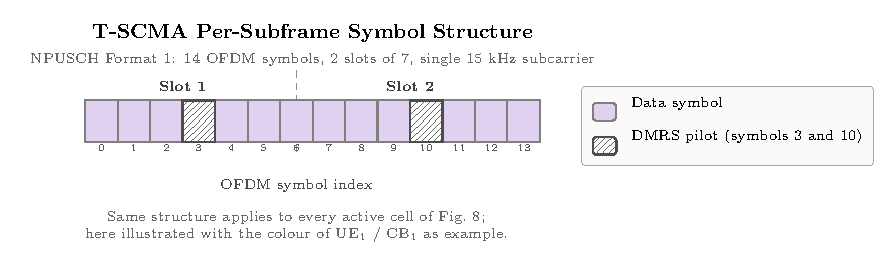
\includegraphics[width=0.92\textwidth]{fig9_tscma_symbol.pdf}
  \caption{Estructura de símbolo dentro de un subframe activo (NPUSCH Format~1, 15~kHz). El subframe se compone de catorce símbolos OFDM organizados en dos slots de siete. Los pilotos DMRS ocupan los símbolos 3 y 10; los doce símbolos restantes transportan datos. La estructura es idéntica para cada celda activa de la \cref{fig:tscma_multiplex}; aquí se ilustra con el color del UE$_1$/CB$_1$ a modo de ejemplo.}
  \label{fig:tscma_symbol}
\end{figure}

Las decisiones de diseño para T-SCMA son:
\begin{description}[leftmargin=1.5em,style=nextline]
  \item[Dominio del tiempo en lugar de frecuencia:] NB-IoT opera con una única subportadora uplink de 15~kHz, lo que imposibilita la multiplexación en frecuencia clásica. El tiempo (subframes) es el único eje disperso disponible.
  \item[Cuatro subframes:] se alinea con la estructura estándar de NPUSCH Format~1 (2 slots de 7 símbolos cada uno). Permite mantener la compatibilidad con la especificación PHY sin modificaciones.
  \item[Piloto DMRS por UE:] cada UE transmite su DMRS en los símbolos 3 y 10 de los subframes en los que su codebook está activo. Las secuencias DMRS son ortogonales entre sí (hasta un máximo de 3 por capa), lo que permite al receptor distinguir las contribuciones individuales superpuestas.
  \item[Superposición en el aire:] las señales de los UEs activos en un mismo subframe se suman coherentemente en el canal. El eNB recibe una única forma de onda compuesta por subframe.
\end{description}

\paragraph{Procedimiento T-SCMA en cinco pasos.} \textbf{(i)}~Cada UE recibe un codebook entre los $K = 6$ disponibles. \textbf{(ii)}~El UE mapea sus datos a una palabra-código de longitud $N = 4$ con solo $d_v = 2$ posiciones no nulas (esparsidad temporal). \textbf{(iii)}~En cada uno de sus dos subframes asignados, el UE transmite símbolos de datos en las posiciones de datos e inserta su propio piloto DMRS en los símbolos 3 y 10 (\cref{fig:tscma_symbol}). \textbf{(iv)}~Hasta $d_f = 3$ UEs transmiten en paralelo en un mismo subframe; los datos se superponen en el aire y los pilotos DMRS, con secuencias Zadoff--Chu distintas, permanecen separables. \textbf{(v)}~El eNB captura una única forma de onda compuesta por subframe, correlaciona contra las secuencias DMRS conocidas para detectar UEs activos y estimar canales, y aplica MPA iterativo para separar los datos superpuestos.

\section{Lógica de resolución MSG3 en el eNB}
\label{sec:resolucion}

La decodificación MSG3 en el eNB sigue una lógica de tres niveles que clasifica cada transmisión recibida como \emph{scheduled}, \emph{contender con colisión de piloto}, o \emph{contender decodificable por MPA}. La \cref{fig:decision} presenta el árbol de decisión formal.

\begin{figure}[H]
  \centering
  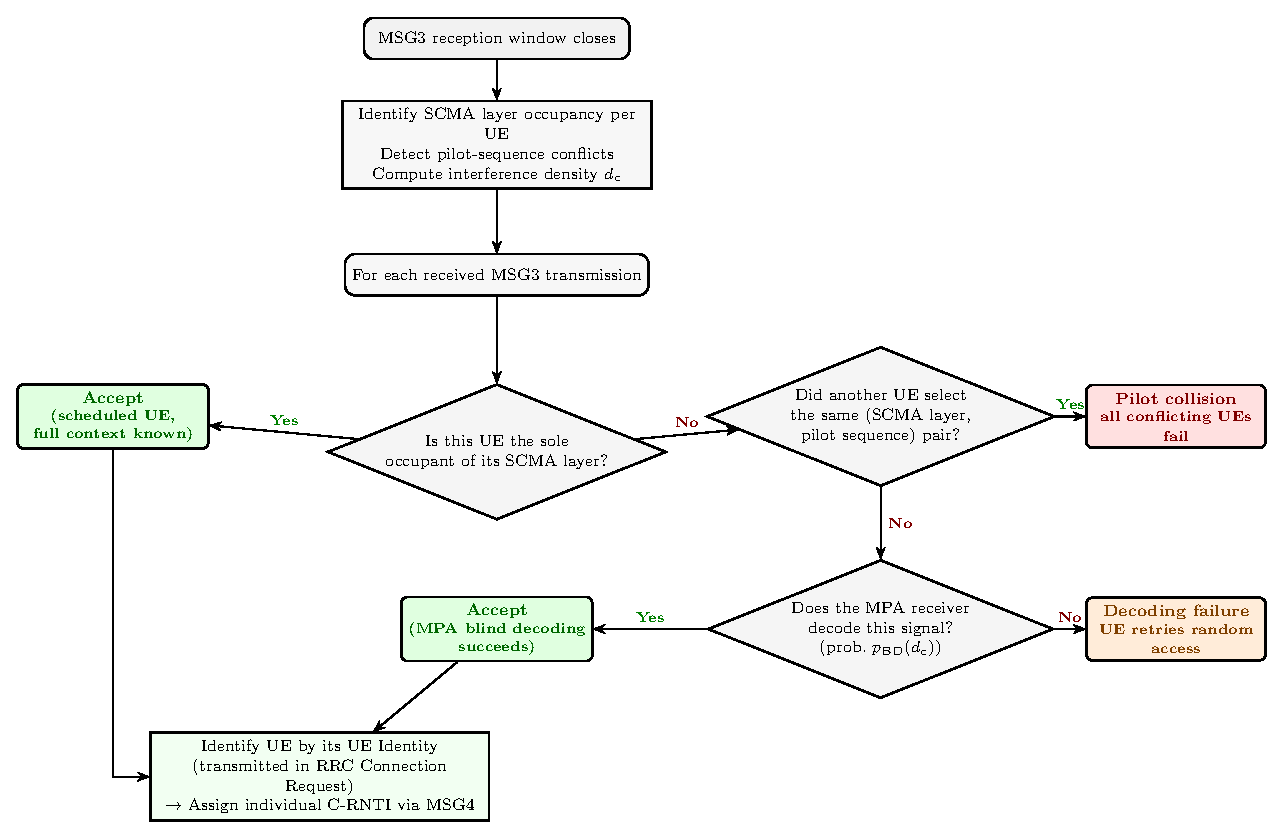
\includegraphics[width=0.90\textwidth]{fig7_decision_tree.pdf}
  \caption{Árbol de decisión del procedimiento de resolución MSG3 en el eNB. Cada transmisión recibida se clasifica en uno de los cuatro casos posibles según si el UE es único en su capa SCMA, si sufre colisión de piloto, o si su señal es decodificable por MPA con probabilidad $p_{\text{BD}}(d_c)$.}
  \label{fig:decision}
\end{figure}

La lógica procede así. Tras cerrarse la ventana de recepción de MSG3, el eNB identifica, para cada capa SCMA, cuántos UEs la están ocupando y qué pilotos DMRS han utilizado. Luego, para cada transmisión recibida:
\begin{enumerate}[leftmargin=*]
  \item \textbf{¿El UE es único ocupante de su capa SCMA?} Si es así, el UE se declara \emph{scheduled}: el eNB conoce totalmente el contexto de su transmisión y la decodifica con probabilidad $p_{\text{BD}} = 1$, sin invocar MPA.
  \item \textbf{¿Otro UE seleccionó la misma pareja (capa, piloto)?} Si es así, ocurre \emph{colisión de piloto}: ambos UEs son indistinguibles para el receptor y ambos fallan. Deberán reintentar el acceso.
  \item \textbf{¿El receptor MPA decodifica la señal?} En otro caso, el eNB invoca MPA sobre el grafo de factores; la probabilidad de decodificación $p_{\text{BD}}(d_c)$ depende del nivel de superposición $d_c$ de la capa. Un resultado exitoso produce el payload del UE y permite la asignación de C-RNTI; un fallo genera un reintento.
\end{enumerate}

La \cref{tab:msg3_casos} resume los cuatro casos posibles y la acción correspondiente del eNB.

\begin{table}[H]
\centering
\caption{Casos de resolución MSG3 en el eNB.}
\label{tab:msg3_casos}
\small
\begin{tabularx}{\textwidth}{@{}l c X X X@{}}
\toprule
\textbf{Caso} & \textbf{Aplica a} & \textbf{Condición} & \textbf{Acción del eNB} & \textbf{Resultado del UE} \\
\midrule
Éxito directo & CRACS-T & UE único en su capa SCMA asignada (clúster con un solo UE) & Aceptar sin invocar MPA & C-RNTI asignado \\
Éxito por MPA & ambas & Pilotos DMRS distintos en la misma capa & MPA converge con $\mathrm{LLR} \geq$ umbral & C-RNTI asignado \\
Colisión de piloto & ambas & Dos o más UEs con misma pareja (capa, piloto) & Descarte de todos los involucrados & Retransmisión tras backoff \\
Fallo de decodificación & ambas & MPA no converge o densidad $d_c$ excesiva & NACK implícito (no emite MSG4) & Retransmisión tras backoff \\
\bottomrule
\end{tabularx}
\end{table}

El caso \emph{Éxito directo} (UE único en su capa SCMA) solo aplica a \textbf{CRACS-T}: la asignación determinista de codebook por clúster permite que algunos UEs sean los únicos ocupantes de su capa, evitando la invocación de MPA. En \textbf{CRACS-R} todos los UEs comparten el catálogo de codebooks vía sorteo aleatorio, por lo que cualquier UE colisionante siempre necesita resolución por MPA (o falla por colisión de piloto).

La probabilidad $p_{\text{BD}}(d_c)$ se modela como una función decreciente del número de UEs activos simultáneamente en la capa (densidad de colisión $d_c$). La \cref{tab:pbd_calib} resume los valores de referencia adoptados, calibrados empíricamente sobre la base de la literatura SCMA y de las corridas iniciales de la fase de evaluación.

\begin{table}[H]
\centering
\caption{Probabilidad de decodificación blind $p_{\text{BD}}(d_c)$ del receptor MPA.}
\label{tab:pbd_calib}
\small
\renewcommand{\arraystretch}{1.15}
\begin{tabular}{@{}c c l@{}}
\toprule
$d_c$ & $p_{\text{BD}}$ & Régimen operativo \\
\midrule
$\leq 2$ & $1{,}00$ & Por debajo de la carga nominal \\
$3$      & $0{,}95$ & Carga nominal, cerca de ML \\
$4$      & $0{,}85$ & Un contendor añadido \\
$5$      & $0{,}70$ & Dos contendores añadidos \\
$\geq 6$ & $\leq 0{,}05$ & Sobrecarga severa \\
\bottomrule
\end{tabular}
\end{table}

En la \cref{fig:decision} solo aparecen los nombres de los nodos de decisión y las acciones resultantes; las probabilidades específicas se consultan en la \cref{tab:pbd_calib}.

\section{Indicadores de desempeño del diseño}
\label{sec:design_kpis}

La evaluación del diseño se apoya en un conjunto de indicadores clave de desempeño (KPIs) que cuantifican la calidad del procedimiento de acceso desde tres perspectivas complementarias: \emph{éxito} (cuántos UEs completan el acceso), \emph{latencia} (cuánto tarda el acceso exitoso) y \emph{eficiencia} (qué costo tiene en reintentos y colisiones). Adicionalmente, CRACS-T expone un indicador propio de calidad del agrupamiento espacial. La \cref{tab:design_kpis} formaliza las definiciones; estos KPIs son los que se reportan en el capítulo de resultados (\cref{ch:resultados}).

\begin{table}[H]
\centering
\caption{Indicadores clave de desempeño (KPIs) del procedimiento de acceso.}
\label{tab:design_kpis}
\small
\begin{tabularx}{\textwidth}{@{}l c X l@{}}
\toprule
\textbf{KPI} & \textbf{Símbolo} & \textbf{Definición} & \textbf{Unidad} \\
\midrule
Tasa de acceso exitoso & SAR & Fracción de UEs que completan MSG1--MSG5 dentro de $\mathrm{PT}_{\max}$ intentos & $[0, 1]$ \\
\addlinespace
SAR de primer intento & $\text{SAR}_{1}$ & Fracción de UEs que completan el acceso en el primer envío de MSG1 & $[0, 1]$ \\
\addlinespace
Latencia de acceso & $T_{\text{access}}$ & Tiempo entre MSG1 y MSG4 sobre UEs exitosos. Se reporta media, mediana ($p50$) y percentil 95 ($p95$) & ms \\
\addlinespace
Latencia del intento exitoso & $T_{\text{inst}}$ & Tiempo entre el último MSG1 (el que tuvo éxito) y MSG4. La diferencia $T_{\text{access}} - T_{\text{inst}}$ cuantifica el costo de los reintentos & ms \\
\addlinespace
Probabilidad de éxito antes de $T$ (SDP) & $\mathrm{SDP}(T)$ & Fracción del \emph{total} de UEs (incluidos fallidos) que completaron el acceso en tiempo $\leq T$. Métrica conjunta latencia--confiabilidad ($T \in \{1, 3, 10\}$\,s) & $[0, 1]$ \\
\addlinespace
Tiempo total de servicio & TST & \emph{Makespan} de la oleada: $\max(t_{\text{MSG4}}) - \min(t_{\text{MSG1}})$ sobre UEs exitosos & ms \\
\addlinespace
ECDF del retardo de acceso & --- & Distribución empírica acumulada del retardo de acceso por esquema, normalizada por el total de UEs (satura en el SAR) & --- \\
\addlinespace
Tasa de colisión de preámbulo & $\mathrm{PCR}_{\text{pre}}$ & Fracción de transmisiones MSG1 que comparten preámbulo con otra transmisión simultánea & $[0, 1]$ \\
\addlinespace
Tasa de colisión de piloto MSG3 & $\mathrm{PCR}_{\text{msg3}}$ & Fracción de transmisiones MSG3 que comparten la misma pareja (capa SCMA, piloto DMRS) con otra en la misma ventana & $[0, 1]$ \\
\addlinespace
Throughput de acceso & $\eta_{\text{ra}}$ & Accesos exitosos por segundo & UE/s \\
\addlinespace
Reintentos & $\text{RTX}_{\text{mean}}$, $\text{RTX}_{\text{max}}$ & Promedio y peor caso de envíos de MSG1 por UE antes del éxito o agotamiento & --- \\
\addlinespace
Identificación correcta de clúster & CID & Fracción de UEs cuyo clúster asignado por el eNB coincide con la partición geométrica de referencia. Solo aplica a CRACS-T & $[0, 1]$ \\
\bottomrule
\end{tabularx}
\end{table}

\section{Regiones operativas esperadas (hipótesis ex-ante)}
\label{sec:design_regiones}

Como hipótesis \emph{ex-ante} del diseño, los tres esquemas cubren regiones operativas de tamaño progresivamente mayor en el plano \emph{(carga $K$, RTT del enlace)}. La \cref{fig:regiones} visualiza esta hipótesis: el esquema Legacy opera con éxito únicamente en cargas bajas y RTT cortos; CRACS-R amplía el rango de carga aceptable mediante la multiplexación SCMA de MSG3; y CRACS-T extendería además la tolerancia al RTT al desacoplar la separación temporal del MSG3 mediante el agrupamiento espacial previo, sustituyendo el sorteo aleatorio de codebook por una asignación determinista por clúster.

\begin{figure}[H]
  \centering
  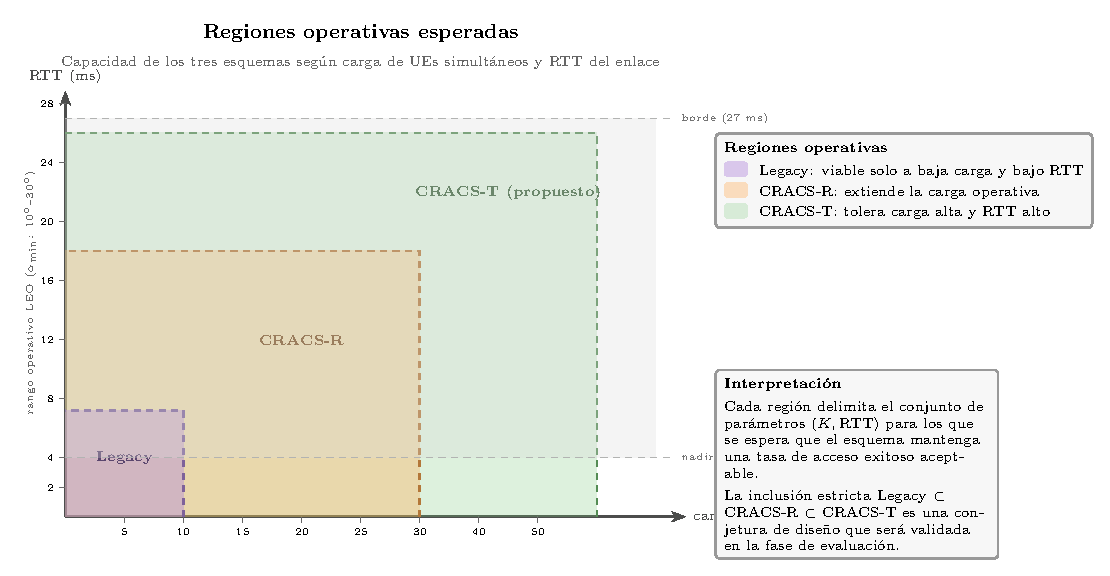
\includegraphics[width=0.95\textwidth]{fig_m2_param_map.pdf}
  \caption{Regiones operativas esperadas de los tres esquemas en función de la carga $K$ y el RTT del enlace. Se conjetura la inclusión estricta Legacy $\subset$ CRACS-R $\subset$ CRACS-T, hipótesis ex-ante que será contrastada experimentalmente en el \cref{ch:resultados}.}
  \label{fig:regiones}
\end{figure}

Formalmente, denotando $\Omega_X \subset \mathbb{R}^2$ la región de parámetros $(K, \mathrm{RTT})$ donde el esquema $X$ mantiene $\mathrm{SAR} \geq \mathrm{SAR}_{\text{umbral}}$, se conjetura la inclusión
\begin{equation}
  \Omega_{\text{Legacy}} \subsetneq \Omega_{\text{CRACS-R}} \subsetneq \Omega_{\text{CRACS-T}},
  \label{eq:inclusion}
\end{equation}
con inclusiones estrictas. Esta conjetura define el horizonte de éxito del diseño propuesto. \emph{Su validez se contrasta empíricamente en el \cref{ch:resultados}, donde los datos revelan que la inclusión es condicional al timer T300 --- un hallazgo no anticipado por el diseño que refina el espacio operativo de la familia CRACS.}

\section{Criterios de aceptación del diseño}
\label{sec:design_criterios}

Los esquemas propuestos se consideran satisfactorios si los resultados experimentales cumplen los siguientes criterios cuantitativos \emph{ex-ante} sobre los KPIs definidos en la \cref{sec:design_kpis}:

\begin{enumerate}[leftmargin=*]
  \item \textbf{Mejora en tasa de acceso:} $\mathrm{SAR}_{\text{CRACS-T}} > \mathrm{SAR}_{\text{CRACS-R}}$ para toda carga $K \geq 3$, con intervalo de confianza al $95\%$.
  \item \textbf{Costo de latencia aceptable:} $T_{\text{access, CRACS-T}} \leq 1{,}1 \cdot T_{\text{access, CRACS-R}}$ en los mismos escenarios; CRACS-T no debe introducir un aumento de latencia superior al $10\%$ respecto a CRACS-R.
  \item \textbf{Precisión del agrupamiento (CRACS-T):} $\mathrm{CID} \geq 0{,}95$ para $\Delta d_{\min} = 150$~m bajo distribución espacial uniforme. Una degradación bajo este umbral exige revisar el parámetro de agrupamiento.
  \item \textbf{Reducción de colisión de piloto:} $\mathrm{PCR}_{\text{msg3, CRACS-T}} \leq 0{,}5 \cdot \mathrm{PCR}_{\text{msg3, CRACS-R}}$ para toda carga $K$. Esta reducción refleja el efecto del agrupamiento determinista sobre la contienda residual en MSG3.
  \item \textbf{Escalabilidad:} ambas propuestas deben mantener $\mathrm{SAR} \geq 0{,}8$ para $K \leq K_{\text{CB}} = 6$ (régimen operativo nominal) y degradar de forma progresiva para cargas superiores.
\end{enumerate}

El no cumplimiento de cualquiera de estos criterios indica una limitación del diseño en el rango operativo correspondiente y debe documentarse explícitamente en la fase de análisis. \emph{La validez condicional de estos criterios --- en particular C1 y C2, que dependen del timer T300 según se muestra en el \cref{ch:resultados} --- se discute en detalle en el capítulo de resultados.}

\section{Plan de evaluación}
\label{sec:metodologia}

Esta sección operacionaliza la fase de pruebas del modelo en cascada descrito en la \cref{sec:metodologia_desarrollo}: define cómo se evalúa el diseño con independencia del entorno de implementación. Se especifican las variables del experimento, los escenarios de evaluación y las condiciones de borde. Las métricas de desempeño son los KPIs ya definidos en la \cref{sec:design_kpis} y los criterios de aceptación contra los que se contrastan los resultados son los enunciados en la \cref{sec:design_criterios}; ninguno se repite aquí.

\subsection{Diseño experimental}
\label{sec:dis_simulacion}

La fase de evaluación se operacionaliza, con independencia del entorno de implementación, manipulando un conjunto de variables sobre el sistema diseñado. Las \textbf{variables independientes} son: la carga $K$ (número de UEs activos en la ventana de acceso); el modelo de tráfico (Poisson uniforme, 3GPP TR~37.868 TM1, o Beta$(3,4)$ sincronizado, TM2); el perfil de tráfico (\emph{avg} moderado o \emph{high} intenso, $\lambda \approx 27{,}8$~UEs/s); la distancia diferencial mínima de agrupamiento $\Delta d_{\min}$ (propia de CRACS-T); el número de preámbulos NPRACH $N_{\text{pream}}$; el temporizador RRC $T_{300}$ (valores estándar NB-IoT, 3GPP TS~36.331); y el esquema bajo prueba (Legacy, CRACS-R o CRACS-T). Los demás parámetros geométricos del enlace ($h_{\text{sat}}$, $\alpha_{\min}$, FSPL constante) se fijan en los valores de referencia documentados en la \cref{sec:modelo_sistema}, ya que el alcance del trabajo es la capacidad del canal de acceso bajo una geometría LEO de referencia y no la sensibilidad a las variables de canal. Las \textbf{variables dependientes} son los KPIs definidos en la \cref{sec:design_kpis} (\cref{tab:design_kpis}).

\textbf{Modelos estadísticos y condiciones de ejecución.} Cada UE inicia su acceso en un instante aleatorio dentro de la ventana $T_{\text{arrival}}$, según la distribución uniforme (caso base) o Beta$(3,4)$ (caso mMTC, 3GPP TR~37.868); los UEs se ubican uniformemente en el disco de cobertura definido por $\alpha_{\min}$ ---distribución espacial neutra, que no privilegia ninguna zona de la huella y representa un despliegue IoT rural sin agrupamiento geográfico previo--- y permanecen estáticos durante cada ejecución independiente del simulador, denominada en adelante \emph{corrida}. Los que fallan un intento reintentan con backoff uniforme hasta un máximo de $\mathrm{PT}_{\max}=10$ intentos, tras lo cual se consideran perdidos. Cada punto experimental se repite con al menos $R=30$ semillas independientes y se reporta como media con intervalo de confianza al 95\% (método $t$ de Student); el tiempo simulado de referencia es $T_{\text{sim}}=120$~s por experimento, suficiente para que todos los UEs completen el procedimiento o agoten sus reintentos. Por corrida se registran los eventos de la cadena MSG1--MSG5 con sus metadatos (UE ID, RAPID, TC-RNTI, capa SCMA, piloto DMRS), que el post-procesamiento agrega por escenario y esquema para calcular los KPIs.

\subsection{Escenarios de evaluación}
\label{sec:escenarios}

Cada escenario aísla una variable independiente y barre su rango manteniendo las demás en los valores de referencia; las variantes \emph{\_high} repiten el barrido bajo el perfil de tráfico intenso ($\lambda \approx 27{,}8$~UEs/s), que satura el canal de acceso. La \cref{tab:escenarios} los resume; la operacionalización exacta de cada uno sobre el simulador se detalla en el \cref{ch:implementacion}.

\begin{table}[H]
\centering
\caption{Escenarios de evaluación.}
\label{tab:escenarios}
\small
\begin{tabularx}{\textwidth}{@{}l l l l X@{}}
\toprule
\textbf{ID} & \textbf{Variable} & \textbf{Rango} & \textbf{Esquemas} & \textbf{Propósito} \\
\midrule
E0 & $K$ & 1 UE & los 3 & \emph{Sanity}: equivalencia de los tres esquemas sin contienda \\
\addlinespace
E1 & $K$ (perfil avg) & 1--100 UEs & los 3 & Curva de capacidad bajo tráfico moderado \\
\addlinespace
E1\_high & $K$ (perfil high $2\text{h}$) & 1--100 UEs & los 3 & Curva de capacidad bajo tráfico intenso \\
\addlinespace
E4 & $\Delta d_{\min}$ (perfil avg) & 50--1000 m & CRACS-T & Calibración del parámetro de agrupamiento \\
\addlinespace
E4\_high & $\Delta d_{\min}$ (perfil high) & 50--1000 m & CRACS-T & Idem bajo tráfico intenso \\
\addlinespace
E5 & $N_{\text{pream}}$ (perfil avg) & 12, 24, 36, 48 & los 3 & Sensibilidad al pool de preámbulos NPRACH \\
\addlinespace
E5\_high & $N_{\text{pream}}$ (perfil high) & 12, 24, 36, 48 & los 3 & Idem bajo tráfico intenso \\
\addlinespace
E6\_uniform & $K$ (Poisson TM1, $T=60$\,s) & 30, 100, 300, 1000 & los 3 & Saturación con tráfico no correlacionado \\
\addlinespace
E6\_burst & $K$ (Beta$(3,4)$ TM2, $T=10$\,s) & 30, 100, 300, 1000 & los 3 & Saturación con ráfaga sincronizada \\
\addlinespace
E7\_t300 & $T_{300}$ (en E6\_burst $K{=}300$) & 5, 10, 40 s & los 3 & Sensibilidad al timer T300 en el punto de cruce \\
\bottomrule
\end{tabularx}
\end{table}

\subsection{Condiciones de borde}
\label{sec:borde}

La evaluación incluye un conjunto de casos límite de control: con $K=1$ los tres esquemas deben comportarse idénticamente, pues no hay colisión posible (cualquier divergencia indicaría un defecto de modelado); para $K > K_{\text{CB}} = 6$ ambas propuestas deben degradar de forma controlada, lo que delimita el rango operativo máximo; cuando todos los UEs caen en un único clúster ($\Delta d < \Delta d_{\min}$), el comportamiento de CRACS-T converge al de CRACS-R; y con $p_{\text{fa}} > 0$ se observa el impacto de las falsas alarmas del detector probabilístico sobre la asignación de RARs.

\chapter{Implementación}
\label{ch:implementacion}

\section{Selección del entorno de simulación}
\label{sec:impl_herramientas}

La implementación del diseño formalizado en el \cref{ch:diseno} requería una plataforma capaz de modelar con suficiente granularidad la pila de protocolos NB-IoT ---en particular las capas MAC y RRC del procedimiento de acceso aleatorio--- e incorporar componentes propios para el escenario LEO no terrestre. Como parte de la búsqueda de herramientas se consideraron tres alternativas representativas en la práctica académica. La \cref{tab:impl_herramientas} contrasta esos tres entornos a través de cinco criterios alineados con los requerimientos del trabajo.

\begin{table}[H]
\centering
\caption{Comparativa de entornos de simulación de redes considerados.}
\label{tab:impl_herramientas}
\small
\renewcommand{\arraystretch}{1.25}
\begin{tabular}{@{}>{\raggedright\arraybackslash}p{3.2cm}
                 >{\raggedright\arraybackslash}p{3.9cm}
                 >{\raggedright\arraybackslash}p{3.9cm}
                 >{\raggedright\arraybackslash}p{3.9cm}@{}}
\toprule
\textbf{Criterio} & \textbf{ns-3 v3.32} & \textbf{OMNeT++ / INET} & \textbf{5G-LENA-NTN} \\
\midrule
Granularidad PHY/MAC & Modelo discreto a nivel de paquete con módulos LTE/NB-IoT maduros. & Modular, con \emph{frameworks} externos (INET, SimuLTE, Veins). & Granularidad NR a nivel de paquete, heredada del módulo NR de ns-3. \\
\addlinespace
Soporte NB-IoT & Implementación nativa en el módulo LTE; extensiones comunitarias para NB-IoT. & Soporte parcial vía SimuLTE (LTE); no incluye NB-IoT nativo. & Enfocado en NR 5G no terrestre; no incluye NB-IoT (centrado en eMBB/URLLC). \\
\addlinespace
Modelo de movilidad satelital & Modelos orbitales LEO disponibles de fábrica. & Modelos genéricos; los satélites requieren desarrollo propio. & Modelos LEO/MEO/GEO nativos (modelo de canal NTN 3GPP TR~38.811). \\
\addlinespace
Costo computacional & Ejecución secuencial; aceptable para escenarios medianos. & Similar a ns-3; más pesado en componentes gráficos. & Mayor que ns-3 LTE por el detalle de la capa NR. \\
\addlinespace
Documentación y comunidad & Extensa, con publicaciones y módulos contribuidos. & Amplia en redes industriales y vehiculares. & Activa pero más reciente; foco en NR. \\
\bottomrule
\end{tabular}
\end{table}

El análisis criterio por criterio orienta la elección con claridad. En granularidad PHY/MAC los tres entornos son comparables a nivel de paquete, pero la pila NR de 5G-LENA-NTN no resuelve el problema del acceso aleatorio en NB-IoT, y la modularidad de OMNeT++ exige integrar y mantener \emph{frameworks} externos. En soporte NB-IoT la diferencia es categórica: solo ns-3 cuenta con una implementación nativa del procedimiento; las otras dos exigirían portarlo desde cero. En el modelo de movilidad satelital, ns-3 dispone de modelo orbital LEO y modelo de propagación LEO listos para usar; OMNeT++ los requeriría como desarrollo propio; 5G-LENA-NTN incorpora un modelo de canal NTN más detallado pero en una pila tecnológica distinta. En costo computacional las tres opciones son equivalentes y aceptables para los volúmenes esperados. En documentación y comunidad, ns-3 lidera por su tradición académica.

A partir de este análisis se seleccionó ns-3 versión 3.32 como plataforma principal por dos razones. Primero, su módulo LTE incluye un procedimiento de acceso aleatorio NB-IoT funcional con estructuras MAC y RRC adaptables, lo que evita portar el procedimiento completo. Segundo, ns-3 proporciona de fábrica un modelo de movilidad orbital y un modelo de propagación LEO que se integran de forma nativa con la simulación a nivel de paquete.

Se descartaron las dos alternativas modernas por razones complementarias. 5G-LENA-NTN aporta un modelo de canal NTN más maduro, pero su pila NR de nueva generación no contempla NB-IoT y habría exigido una migración significativa fuera del alcance del trabajo de grado. OMNeT++ con INET ofrece una capa MAC LTE modular, pero tampoco implementa NB-IoT de forma nativa y obligaba a portar el procedimiento completo. Por estas razones se mantuvo ns-3 como base.

\section{Consideraciones y limitaciones de implementación}
\label{sec:impl_limitaciones}

Durante la fase de implementación se hicieron explícitas tres clases de restricciones que acotan el alcance de la simulación.

\paragraph{Restricciones computacionales:} ns-3 ejecuta sus eventos de manera secuencial sobre un solo hilo. Una ejecución de 120~s simulados con pocos UEs activos toma del orden de segundos de tiempo de cómputo. La fase experimental requiere miles de ejecuciones para construir intervalos de confianza con 30 semillas por punto, lo que se afronta mediante paralelización externa de procesos independientes (\cref{sec:impl_recoleccion}).

\paragraph{Simplificaciones de alcance del modelo:} el simulador implementa un único satélite LEO sirviendo a una población de UEs estacionarios sobre un único Bloque de Recursos Físicos (PRB) de 180~kHz, que contiene 12 subportadoras espaciadas a 15~kHz. El NPRACH ocupa hasta esas 12 subportadoras físicas; el pool de preámbulos se barre entre 12, 24, 36 y 48 valores en el espacio lógico de 3{,}75~kHz, con cuatro preámbulos virtuales por subportadora física. La transmisión MSG3 es multi-tono. Lo que no se barre dinámicamente es el ancho de banda asignado al canal de acceso: se mantiene constante en 1~PRB durante toda la campaña. La propagación se modela como línea de vista con pérdidas constantes (atmosférica, espacio libre y margen) y un criterio de cobertura de tipo todo-o-nada según el ángulo de elevación mínimo. No se modelan desvanecimiento rápido, sombreado, ni desplazamiento Doppler. Estos supuestos se documentan en detalle en la \cref{sec:modelo_sistema} y acotan el alcance de validez de los resultados que siguen.

\paragraph{Compatibilidad con la base ns-3:} la extensión del módulo LTE se construyó sobre los componentes reutilizados de ns-3 (capa RLC, dispositivos de red y \emph{helpers} EPC) sin modificarlos, para no bifurcar la base de código y mantener la simulación apoyada en partes ya validadas por la comunidad. Esto condicionó algunas decisiones de diseño, que respetaron las interfaces existentes de esos componentes.

\section{Arquitectura de la implementación}
\label{sec:impl_arquitectura}

La implementación se organizó por componentes y distingue tres orígenes distintos. Los componentes \emph{reutilizados} provienen directamente de la base ns-3 y no se modificaron, lo que asegura que su comportamiento ya esté validado por la comunidad. Los componentes \emph{extendidos} parten de una implementación existente pero se adaptaron para reflejar con mayor fidelidad las condiciones del escenario NB-IoT no terrestre o para no introducir sesgos a favor de un esquema. Los componentes \emph{nuevos} fueron desarrollados como aporte original del trabajo e implementan los algoritmos y abstracciones propuestos en el diseño. La \cref{tab:impl_componentes} consolida este mapeo con su correspondencia a las secciones del capítulo de diseño y la categoría de origen.

\begin{table}[H]
\centering
\caption{Mapeo entre los bloques del diseño y los componentes implementados.}
\label{tab:impl_componentes}
\small
\renewcommand{\arraystretch}{1.2}
\begin{tabularx}{\textwidth}{@{}>{\raggedright\arraybackslash}p{4.5cm} >{\raggedright\arraybackslash}X >{\raggedright\arraybackslash}p{2.0cm}@{}}
\toprule
\textbf{Bloque del diseño} & \textbf{Componente implementado} & \textbf{Origen} \\
\midrule
Modelo orbital y geometría LEO (\cref{sec:modelo_sistema}) & Modelo orbital LEO, modelo de propagación LEO y modelo de retardo de propagación constante, disponibles de fábrica en ns-3. & Reutilizado \\
Movilidad estacionaria de UEs (\cref{sec:modelo_sistema}) & Modelo de posición constante con asignación uniforme en disco, disponibles de fábrica. & Reutilizado \\
\midrule
Generación de tráfico (\cref{sec:modelo_sistema}) & Generador de arribos extendido para soportar los dos modelos de tráfico mMTC (\cref{sec:impl_trafico}). & Extendido \\
Procedimiento Legacy (\cref{sec:legacy}) & Rama base del MAC NB-IoT, adaptada en el manejo de colisiones para reflejar el costo real del recurso en el aire (ver discusión al final de esta sección). & Extendido \\
\midrule
Detector probabilístico (\cref{sec:cracs_r,sec:cracs_t}) & Sub-rutina del MAC del eNB que invoca el detector y propaga la decisión al flujo de RAR (\cref{alg:detector}). & Nuevo \\
Esquema CRACS-R (\cref{sec:cracs_r}) & Rama de procedimiento con dos RAR fijas y resolución MSG3 propia. & Nuevo \\
Esquema CRACS-T (\cref{sec:cracs_t}) & Rama de procedimiento con \emph{clustering} ToA previo, una RAR por clúster y resolución MSG3 propia. & Nuevo \\
\emph{Clustering} ToA (\cref{sec:toa}) & Algoritmo de barrido ordenado sobre distancias diferenciales (\cref{alg:clustering}). & Nuevo \\
Lógica de decisión MSG3 (\cref{sec:resolucion}) & Clasificador de transmisiones por densidad efectiva en el factor graph (\cref{alg:decision}). & Nuevo \\
Decodificador SCMA / MPA (\cref{sec:scma}) & Modelo abstracto a nivel de sistema basado en probabilidad tabulada (\cref{alg:mpa}). & Nuevo \\
Modelado SCMA (asignación de codebook) & Determinista por clúster ToA en CRACS-T; sorteo aleatorio del catálogo en CRACS-R; ambos sobre la misma matriz factorial $\mathbf{F}_{4\times 6}$ y $K_{\text{CB}}=6$ capas. & Nuevo \\
\emph{Helper} de temporización NTN & Estimación del RTT esperado por UE para alimentar la lógica de \emph{timing advance}. & Nuevo \\
Sistema de reportería interno & Módulo común a los tres esquemas que centraliza los eventos y los KPIs de cada simulación. & Nuevo \\
\bottomrule
\end{tabularx}
\end{table}

La tabla refleja una decisión arquitectónica importante: toda la diferencia entre esquemas reside en componentes nuevos a nivel del MAC del eNB; la pila por encima (RLC, dispositivos de red, EPC) permanece compartida. Esta granularidad preserva la trazabilidad del comportamiento del simulador y simplifica la depuración cruzada entre los tres esquemas, porque cualquier diferencia observada en los KPIs es atribuible a la lógica de acceso aleatorio y no a una asimetría en las capas superiores. La extensión del generador de tráfico es necesaria para soportar los dos modelos mMTC del estándar; la extensión del procedimiento Legacy se justifica a continuación.

\paragraph{Extensión del procedimiento Legacy --- manejo realista de colisiones:} la rama Legacy preserva la lógica del procedimiento NB-IoT original incluido en ns-3, pero se modificó el manejo de las colisiones. En la implementación de base los preámbulos detectados como colisión se descartaban tempranamente, de modo que los UEs implicados no consumían los recursos del procedimiento aguas abajo. Esta simplificación era conveniente pero \emph{optimista}: subestimaba el costo real de una colisión y favorecía artificialmente al baseline en las comparaciones contra los esquemas con SCMA. La implementación actual extiende esa lógica para que las transmisiones colisionantes consuman efectivamente los recursos del procedimiento hasta MSG3 ---emisión de una RAR compartida, transmisión MSG3 sobre PUSCH y recepción posterior--- y sean descartadas en el receptor mediante una decisión explícita. De este modo, una colisión real ocupa los mismos recursos que ocuparía sobre el aire en una red NB-IoT desplegada, lo que produce comparaciones más fieles entre los tres esquemas y elimina el sesgo a favor de Legacy.

\section{Configuración del simulador}
\label{sec:impl_config}

La configuración del simulador se gobierna desde un único punto de entrada que expone los parámetros del experimento como argumentos de línea de comandos. Esta separación permite recorrer todos los escenarios de evaluación sin recompilar.

\paragraph{Parámetros globales:} los parámetros comunes a los tres esquemas se agrupan en cuatro categorías:
\begin{itemize}[leftmargin=*, noitemsep]
  \item \emph{Parámetros orbitales del satélite:} altitud orbital, inclinación, latitud y longitud iniciales del punto sub-satelital y ángulo de elevación mínimo de cobertura.
  \item \emph{Parámetros del canal:} pérdidas atmosférica, de espacio libre y de margen, junto con la velocidad de propagación.
  \item \emph{Parámetros de tráfico:} modelo activo (Poisson o Beta), preset de población virtual, perfil de duración y máximo de arribos por simulación.
  \item \emph{Semilla de aleatoriedad:} permite reproducir cada corrida bit a bit.
\end{itemize}

\paragraph{Parámetros por esquema:} la selección del esquema activo se hace mediante un parámetro categórico, y cada esquema expone sus propios ajustes:
\begin{itemize}[leftmargin=*, noitemsep]
  \item \emph{Legacy:} no expone parámetros adicionales más allá de los globales; es el baseline NB-IoT estándar.
  \item \emph{CRACS-R:} tamaño máximo de grupo SCMA y tamaño del catálogo de pilotos DMRS anunciados.
  \item \emph{CRACS-T:} distancia diferencial mínima $\Delta d_{\min}$ entre clústeres ToA, parámetro central de su mecanismo de agrupamiento.
\end{itemize}

\paragraph{Detector de colisiones:} la probabilidad de detección y la de falsa alarma del detector probabilístico son comunes a CRACS-R y CRACS-T y se exponen como parámetros configurables para permitir el estudio de sensibilidad.

La \cref{tab:impl_flags} consolida los parámetros más relevantes con sus valores de referencia. La tabla preserva el identificador técnico de cada parámetro para que la corrida sea reproducible por quien acceda al simulador, pero el cuerpo del capítulo se refiere a ellos por su rol funcional.

\begin{table}[H]
\centering
\caption{Parámetros del simulador (selección).}
\label{tab:impl_flags}
\small
\renewcommand{\arraystretch}{1.2}
\begin{tabularx}{\textwidth}{@{}>{\raggedright\arraybackslash}p{4.6cm} >{\raggedright\arraybackslash}X >{\raggedright\arraybackslash}p{2.4cm}@{}}
\toprule
\textbf{Parámetro} & \textbf{Descripción} & \textbf{Valor de ref.} \\
\midrule
Esquema activo & Selecciona Legacy, CRACS-R o CRACS-T. & CRACS-R \\
Semilla y \emph{run} de aleatoriedad & Reproducibilidad bit a bit. & 12345, 1 \\
Máximo de arribos & Límite de UEs activos en la ventana de acceso ($0$ = ilimitado, sujeto a la tasa $\lambda$). & 0 \\
Modelo de tráfico & Selecciona TM1 Poisson o TM2 Beta de 3GPP TR~37.868. & Poisson \\
Preset de población y perfil & Población virtual y período (modo Poisson). & avg, 2h \\
Horizonte $T$ de la ráfaga & Duración de la ráfaga sincronizada Beta$(3,4)$ (modo Beta). & 10~s \\
Altitud orbital del satélite & Altitud LEO. & 600~km \\
Elevación mínima de cobertura & Ángulo límite por debajo del cual el UE queda fuera de servicio. & 40\textdegree \\
Pérdidas constantes del enlace & Atmosférica, espacio libre y margen. & 0,53 / 150 / 0,82~dB \\
Detector probabilístico & Probabilidad de detección y de falsa alarma. & 0,975 / 0,001 \\
Pool de preámbulos NPRACH & Tamaño barrido en el espacio lógico de 3,75~kHz, aplicado a los tres niveles CE simultáneamente. & 12 \\
Separación mínima entre clústeres $\Delta d_{\min}$ & Resolución temporal efectiva del NPRACH. & 150~m \\
Parámetros CRACS-R & Tamaño máximo de grupo SCMA y tamaño del catálogo de pilotos DMRS. & 2, 3 \\
Temporizadores RRC T300 y de \emph{Connection Request} & Temporizador T300 del UE y \emph{timeout} del eNB. Valor estándar 5\,000~ms según 3GPP TS~36.331; E7\_t300 lo barre en $\{5\,000,\;10\,000,\;40\,000\}$~ms. & 5\,000 / 5\,000 \\
Tiempo simulado total & Duración de cada corrida. & 120\,000~ms \\
\bottomrule
\end{tabularx}
\end{table}

\subsection{Modelo de tráfico}
\label{sec:impl_trafico}

La generación del tráfico de acceso implementa los dos modelos para mMTC definidos en 3GPP TR~37.868 \S6.1.1. Ambos comparten el parámetro $N$ que fija el número exacto de UEs inicializados en la simulación. La selección entre ellos depende de la pregunta operativa que el escenario pretenda responder.

\paragraph{Traffic Model 1 --- Poisson uniforme:} los inter-arribos se generan con una variable aleatoria exponencial de media $1/\lambda$, donde $\lambda = N_{\text{pop}}/T_{\text{period}}$. Cuando se utiliza el preset \emph{custom}, $N_{\text{pop}}$ es la población virtual configurable (típicamente igual a $N$) y $T_{\text{period}}$ se fija con el horizonte declarado (60~s en el escenario E6\_uniform, alineado con el caso nominal 3GPP). Los presets \emph{avg}, \emph{high} y \emph{ultra} ofrecen valores cerrados (52\,500, 200\,000, 500\,000) combinados con perfiles temporales (7\,200~s, 600~s) para experimentos de carga rápida. Este modelo responde a la pregunta de capacidad estructural bajo carga sostenida, y reproduce el caso de tráfico de fondo no correlacionado donde cada dispositivo opera con su propio reloj.

\paragraph{Traffic Model 2 --- Beta$(3,4)$ sincronizado:} los $N$ instantes de arribo se generan como $t_i = T \cdot X_i$ con $X_i \sim \mathrm{Beta}(\alpha = 3, \beta = 4)$ y horizonte $T$ configurable (10~s en E6\_burst, valor nominal 3GPP). La densidad de arribos tiene un pico en $t^\ast = (\alpha - 1)/(\alpha + \beta - 2) \cdot T = 0{,}4\,T$. La generación interna aprovecha la identidad: si $X \sim \mathrm{Gamma}(\alpha, 1)$ y $Y \sim \mathrm{Gamma}(\beta, 1)$, entonces $X/(X + Y) \sim \mathrm{Beta}(\alpha, \beta)$. Este modelo responde a la pregunta de robustez ante ráfagas sincronizadas por un evento común (corte de luz, alarma masiva, encendido tras período de descanso). En NB-IoT no terrestre representa además el caso normal al inicio de cada ventana de visibilidad satelital, cuando varios UEs intentan acceder simultáneamente al recuperar conectividad.

Los escenarios E6\_uniform y E6\_burst (\cref{tab:escenarios}) barren la misma variable $N \in \{30, 100, 300, 1000\}$ bajo cada modelo, lo que permite contrastar sus efectos sobre los tres esquemas. El tope superior $N = 1000$ se eligió por viabilidad computacional; la especificación 3GPP nominal contempla hasta $N = 30\,000$ y queda fuera del alcance experimental por su costo de simulación, declarándose como trabajo futuro.

\subsection{Distribución espacial de los UEs}
\label{sec:impl_espacial}

Las posiciones iniciales de los UEs se generan mediante una asignación uniforme sobre un disco horizontal de radio $R_{\text{cell}}$ centrado en el origen local; cada posición resultante se proyecta posteriormente al sistema ECEF utilizando como referencia geográfica la latitud y longitud central declaradas. Los UEs son estacionarios durante toda la simulación, mientras que el satélite sí evoluciona en el tiempo a través del modelo orbital LEO.

La implementación actual cubre la distribución uniforme. Una distribución agrupada con varios focos geográficos y dispersión local no está implementada y queda como una extensión natural para evaluaciones de robustez ante no uniformidad espacial.

\section{Desarrollo de módulos}
\label{sec:impl_modulos}

Esta sección detalla los cuatro algoritmos centrales que implementan la lógica nueva del simulador. Cada algoritmo se presenta primero con una breve introducción del problema que resuelve, una descripción verbal de su funcionamiento y, a continuación, el pseudocódigo formal acompañado de su complejidad y el bloque del diseño al que corresponde.

\subsection{Detector probabilístico de colisión}
\label{sec:impl_detector}

El detector se invoca al final de la recepción de los preámbulos NPRACH, antes de decidir cómo construir las RAR. Implementa el mecanismo descrito en la \cref{sec:cracs_r}, común a CRACS-R y CRACS-T, y resuelve el siguiente problema: a partir del estado real de colisión ---observable internamente por el contador de UEs que comparten un mismo identificador de preámbulo (RAPID)---, el detector debe producir una decisión binaria con una tasa de detecciones correctas (TPR) y una tasa de falsas alarmas (FPR) calibradas. La decisión binaria es la que el MAC utiliza para bifurcar entre el flujo de éxito y el flujo de resolución por colisión.

El funcionamiento se basa en un sorteo Bernoulli condicionado al estado real. Si hay colisión real, el detector la reconoce con probabilidad TPR; si no la hay, el detector reporta falsa alarma con probabilidad FPR. De este modo, el simulador refleja la incertidumbre típica de un detector práctico sin depender del proceso físico de correlación de secuencias en banda base. El \cref{alg:detector} formaliza la operación.

\begin{algorithm}[H]
\DontPrintSemicolon
\caption{Detector probabilístico de colisión}
\label{alg:detector}
\KwIn{\texttt{actualCollision} (bool, indica si dos o más UEs comparten RAPID); \texttt{TPR}; \texttt{FPR}}
\KwOut{\texttt{predictedCollision} (bool consumido por el MAC para bifurcar)}
$u \leftarrow \mathrm{Uniform}(0, 1)$\;
\eIf{$\mathtt{actualCollision} = \mathrm{true}$}{
  $\mathtt{predictedCollision} \leftarrow (u < \mathtt{TPR})$ \tcp*[r]{detección con prob. TPR}
}{
  $\mathtt{predictedCollision} \leftarrow (u < \mathtt{FPR})$ \tcp*[r]{falsa alarma con prob. FPR}
}
\Return $\mathtt{predictedCollision}$\;
\end{algorithm}

\noindent\textbf{Complejidad:} $O(1)$ por invocación. La generación uniforme aprovecha el generador de números aleatorios global del simulador, ligado a la semilla configurada.

\subsection{Algoritmo de \emph{clustering} ToA por distancia diferencial}
\label{sec:impl_clustering}

El \emph{clustering} por tiempo de llegada es el aporte algorítmico central de CRACS-T (\cref{sec:cracs_t,sec:toa}). Resuelve el siguiente problema: dadas las distancias diferenciales $\Delta d_i = d_{\text{slant},i} - h_{\text{sat}}$ de los $K$ UEs colisionantes, agruparlos en clústeres disjuntos tales que dentro de un clúster todos los UEs estén dentro de la resolución de ToA $\Delta d_{\min}$ y entre clústeres consecutivos haya al menos esa misma separación. La salida es una asignación de cada UE a un identificador de clúster.

El funcionamiento sigue un barrido ordenado de tipo \emph{single-link}: se ordenan las distancias en orden ascendente y se recorre el vector ordenado, comparando cada UE con el inicio del clúster actual. Si la diferencia supera el umbral $\Delta d_{\min}$, se abre un nuevo clúster que comienza en la distancia del UE actual; si no, el UE se incorpora al clúster en curso. El procedimiento se cierra en una sola pasada lineal sobre los datos ya ordenados. El \cref{alg:clustering} formaliza el procedimiento.

\begin{algorithm}[H]
\DontPrintSemicolon
\caption{\emph{Clustering} ToA por distancia diferencial}
\label{alg:clustering}
\KwIn{$\Delta d[1..K]$ distancias diferenciales de los $K$ UEs colisionantes; $\Delta d_{\min}$ separación mínima entre clústeres}
\KwOut{$\mathtt{clusterId}[1..K]$ asignación de cada UE a un clúster en $\{0, 1, \ldots, M-1\}$}
$\mathtt{sortedIdx} \leftarrow \mathrm{argsort}(\Delta d)$ \tcp*[r]{ordenar por distancia ascendente}
$\mathtt{clusterStart} \leftarrow \Delta d[\mathtt{sortedIdx}[1]]$\;
$\mathtt{currentCluster} \leftarrow 0$\;
$\mathtt{clusterId}[\mathtt{sortedIdx}[1]] \leftarrow 0$\;
\For{$i \leftarrow 2$ \KwTo $K$}{
  $\mathtt{idx} \leftarrow \mathtt{sortedIdx}[i]$\;
  \If{$\Delta d[\mathtt{idx}] - \mathtt{clusterStart} \geq \Delta d_{\min}$}{
    $\mathtt{currentCluster} \leftarrow \mathtt{currentCluster} + 1$ \tcp*[r]{abrir nuevo clúster}
    $\mathtt{clusterStart} \leftarrow \Delta d[\mathtt{idx}]$\;
  }
  $\mathtt{clusterId}[\mathtt{idx}] \leftarrow \mathtt{currentCluster}$\;
}
\Return $\mathtt{clusterId}$\;
\end{algorithm}

\noindent\textbf{Complejidad:} $O(K \log K)$ dominada por la ordenación. La pasada lineal posterior es $O(K)$. La salida produce a lo sumo $\min(K, K_{\text{CB}})$ clústeres porque el número de \emph{codebooks} SCMA disponibles ($K_{\text{CB}} = 6$) actúa como techo operativo.

\subsection{Lógica de decisión MSG3}
\label{sec:impl_decision}

Tras la ventana de cuatro \emph{subframes} en la que llegan las transmisiones MSG3 superpuestas, el eNB debe decidir el destino de cada una. El problema es clasificar cada transmisión en una de cuatro categorías mutuamente excluyentes: \emph{scheduled} cuando es la única en su capa SCMA y por tanto no compite con nadie; \emph{contender\_ok} cuando comparte capa con otras pero el decodificador logra separarlas; \emph{pilot\_collision} cuando además del \emph{codebook} comparte el piloto DMRS con otra y queda indistinguible; y \emph{mpa\_fail} cuando comparte capa pero el decodificador no consigue separarlas.

El funcionamiento del algoritmo descansa en dos histogramas calculados al inicio: el conteo de pares (\emph{codebook}, piloto) y el conteo por \emph{codebook}. Con ellos, la clasificación de cada transmisión se decide en tres pasos: si su \emph{codebook} es único, queda \emph{scheduled} sin más; si su par (\emph{codebook}, piloto) se repite, se etiqueta \emph{pilot\_collision} porque no hay forma de distinguirlas; en cualquier otro caso, se consulta el factor graph para obtener la densidad efectiva $d_c$ en su elemento de recurso, se busca la probabilidad de éxito $p_{\text{BD}}(d_c)$ y se decide \emph{contender\_ok} o \emph{mpa\_fail} mediante un sorteo Bernoulli con esa probabilidad. El \cref{alg:decision} formaliza la operación.

\begin{algorithm}[H]
\DontPrintSemicolon
\caption{Lógica de decisión MSG3 (CRACS-T)}
\label{alg:decision}
\KwIn{Conjunto $\mathcal{T}$ de transmisiones MSG3 recibidas; factor graph $\mathbf{F}_{4 \times 6}$}
\KwOut{$\mathtt{decision}[t] \in \{\mathrm{SCHEDULED}, \mathrm{CONTENDER\_OK}, \mathrm{PILOT\_COLLISION}, \mathrm{MPA\_FAIL}\}$}
$\mathtt{comboCounts} \leftarrow$ histograma de pares $(t.\mathtt{codebook}, t.\mathtt{dmrs})$ sobre $\mathcal{T}$\;
$\mathtt{entriesPerCb} \leftarrow$ histograma de $t.\mathtt{codebook}$ sobre $\mathcal{T}$\;
\ForEach{$t \in \mathcal{T}$}{
  \uIf{$\mathtt{entriesPerCb}[t.\mathtt{codebook}] = 1$}{
    $\mathtt{decision}[t] \leftarrow \mathrm{SCHEDULED}$ \tcp*[r]{único en su capa}
  }
  \uElseIf{$\mathtt{comboCounts}[(t.\mathtt{codebook}, t.\mathtt{dmrs})] > 1$}{
    $\mathtt{decision}[t] \leftarrow \mathrm{PILOT\_COLLISION}$ \tcp*[r]{misma capa y piloto}
  }
  \Else{
    $d_c \leftarrow \mathrm{computeDensity}(\mathbf{F}, \mathtt{comboCounts}, t)$\;
    $p_{\text{BD}} \leftarrow \mathrm{pBlindDecoding}(d_c)$\;
    $u \leftarrow \mathrm{Uniform}(0, 1)$\;
    $\mathtt{decision}[t] \leftarrow (u < p_{\text{BD}})\ ?\ \mathrm{CONTENDER\_OK}\ :\ \mathrm{MPA\_FAIL}$\;
  }
}
\Return $\mathtt{decision}$\;
\end{algorithm}

\noindent\textbf{Complejidad:} $O(|\mathcal{T}|)$ dominada por la pasada sobre las transmisiones. La construcción de los histogramas y la consulta al factor graph son $O(1)$ amortizados.

\subsection{Modelo abstracto del decodificador MPA}
\label{sec:impl_mpa}

El decodificador SCMA basado en MPA debería simularse iterativamente sobre el grafo factorial, lo cual es costoso a nivel de sistema. El problema operativo es distinto: solo se necesita predecir si la decodificación tiene éxito o no, en función de la densidad efectiva $d_c$ en cada elemento de recurso. Por eso el simulador adopta una abstracción a nivel de sistema: una probabilidad de éxito $p_{\text{BD}}(d_c)$ tabulada en función de $d_c$.

El funcionamiento es directo: dada la densidad efectiva, se devuelve la probabilidad correspondiente según una tabla con valores monótonamente decrecientes. Para los casos de baja contención ($d_c \le 2$) la decodificación es prácticamente segura; en el rango operativo nominal ($d_c \in \{3,4,5\}$) la probabilidad decrece desde $0{,}95$ hasta $0{,}70$; para densidades mayores, la curva continúa con un decaimiento exponencial acotado inferiormente por un piso de $0{,}05$ que evita probabilidades nulas en regímenes de contención muy alta. El \cref{alg:mpa} resume la operación.

\begin{algorithm}[H]
\DontPrintSemicolon
\caption{Modelo abstracto de la decodificación MPA}
\label{alg:mpa}
\KwIn{$d_c$ densidad efectiva en el elemento de recurso (combos activos)}
\KwOut{$p_{\text{BD}}$ probabilidad de éxito de la decodificación blind}
\Switch{$d_c$}{
  \lCase{$0$}{$p_{\text{BD}} \leftarrow 1{,}00$ \tcp*[r]{caso degenerado}}
  \lCase{$1$}{$p_{\text{BD}} \leftarrow 1{,}00$ \tcp*[r]{único, sin interferencia}}
  \lCase{$2$}{$p_{\text{BD}} \leftarrow 1{,}00$ \tcp*[r]{decodificable sin pérdida}}
  \lCase{$3$}{$p_{\text{BD}} \leftarrow 0{,}95$ \tcp*[r]{$d_f$ nominal}}
  \lCase{$4$}{$p_{\text{BD}} \leftarrow 0{,}85$}
  \lCase{$5$}{$p_{\text{BD}} \leftarrow 0{,}70$}
  \lOther{$p_{\text{BD}} \leftarrow \max\bigl(0{,}05,\ 0{,}70 \cdot e^{-0{,}5\,(d_c - 5)}\bigr)$ \tcp*[r]{decaimiento exponencial con piso $0{,}05$}}
}
\Return $p_{\text{BD}}$\;
\end{algorithm}

\noindent La forma del decaimiento exponencial para $d_c \geq 6$ extiende la curva monótona observable en SCMA y queda acotada inferiormente para evitar probabilidades nulas en regímenes de contención extrema. La justificación de la abstracción a nivel de sistema se discute en la \cref{sec:scma}.

\section{Configuración del escenario de pruebas}
\label{sec:impl_escenarios}

El escenario de pruebas instancia el plan de evaluación del diseño en términos concretos del simulador: qué variables se manipulan, qué métricas se observan, qué combinaciones de parámetros se recorren y bajo qué condiciones estadísticas. La definición que sigue se apoya únicamente en las capacidades efectivamente expuestas por el simulador y en los KPIs reportados al final de cada corrida.

\subsection{Variables manipuladas}
\label{sec:impl_vars_indep}

Las variables manipuladas en los experimentos corresponden a los siguientes parámetros del sistema descrito en el \cref{ch:diseno}:
\begin{itemize}[leftmargin=*, noitemsep]
  \item $K$: número de UEs activos en la ventana de acceso.
  \item $h_{\text{sat}}$: altitud orbital del satélite.
  \item $\alpha_{\min}$: ángulo de elevación mínimo de cobertura.
  \item $\Delta d_{\min}$: distancia diferencial mínima entre clústeres ToA, aplicable a CRACS-T.
  \item $N_{\text{pream}}$: tamaño del pool de preámbulos NPRACH disponibles, aplicado simultáneamente a los tres niveles CE para que el pool efectivo no dependa de la geometría del enlace. Las probabilidades del detector $(p_{\text{det}}, p_{\text{fa}}) = (0{,}975,\, 0{,}001)$ se mantienen fijas en el valor calibrado en estudios previos.
  \item Esquema bajo prueba: Legacy, CRACS-R o CRACS-T (variable categórica).
  \item Intensidad del tráfico: controlada conjuntamente por el preset de población y el perfil temporal, que determinan la tasa media $\lambda$ del proceso de arribos.
\end{itemize}

\subsection{Variables observadas}
\label{sec:impl_vars_dep}

Las variables observadas son los seis KPIs cuyas definiciones formales aparecen en la \cref{sec:design_kpis}: SAR, $T_{\text{access}}$, PCR\textsubscript{pre}, PCR\textsubscript{msg3}, RTX y CID. Cada KPI se reporta con su valor agregado por simulación en los archivos de salida del simulador, junto con los datos por UE que permiten reconstruir distribuciones detalladas.

\paragraph{Reporte objetivo de la latencia:} el tiempo de acceso $T_{\text{access}}$, definido como el intervalo entre el primer preámbulo MSG1 y la recepción de MSG4, solo existe para los UEs que completan el procedimiento. Por eso, promediarlo de forma aislada introduce un sesgo de supervivencia: un esquema que abandona UEs reporta una latencia artificialmente baja, porque deja fuera los casos más costosos. Para una evaluación objetiva de la latencia ---siguiendo la práctica de la literatura de acceso aleatorio en NB-IoT y mMTC--- la latencia se reporta mediante tres instrumentos complementarios:
\begin{enumerate}[leftmargin=*, noitemsep]
  \item $T_{\text{access}}$ con su media, mediana y percentil~95, presentado siempre junto al SAR;
  \item la función de distribución acumulada empírica del $T_{\text{access}}$, normalizada por el número total de UEs, de modo que la curva satura en el valor del SAR y el sesgo se hace explícito;
  \item la probabilidad de entrega exitosa dentro de un plazo, $\mathrm{SDP}(T) = \#\{\text{UEs con } T_{\text{access}} \le T\} / N$, una métrica conjunta de confiabilidad y latencia evaluada en $T \in \{1,\;3,\;10\}$~s que no requiere asignar un tiempo de acceso ficticio a los UEs fallidos.
\end{enumerate}
Se complementa con el \emph{Total Service Time}, el tiempo total que el sistema necesita para resolver la oleada completa de solicitudes, reportado junto al SAR alcanzado.

\subsection{Mapeo de los escenarios al simulador}
\label{sec:impl_mapeo}

El plan de escenarios de evaluación (\cref{tab:escenarios}) se ejecuta sobre el simulador con los valores de referencia de la \cref{tab:impl_flags}; los valores exactos de cada barrido se reportan junto a su análisis en el \cref{ch:resultados}. Cada combinación se recorre con 30 semillas independientes para construir intervalos de confianza al 95\% basados en la distribución $t$ de Student con $n-1$ grados de libertad.

Las variantes \emph{\_high} (E1\_high, E4\_high, E5\_high) reproducen el barrido de su escenario base bajo el perfil de tráfico intenso ($\lambda \approx 27{,}8$~UEs/s, $\sim$8,9~UEs por ventana NPRACH). A diferencia de un simple aumento de $K$, este perfil eleva la densidad de arribos por ventana de acceso, que es la magnitud que satura realmente el canal de acceso aleatorio y permite separar los esquemas. El escenario E7\_t300 barre el temporizador T300 en el punto de operación de cruce CRACS-R / CRACS-T (E6\_burst $K{=}300$); los tres valores barridos corresponden al rango estándar NB-IoT definido en 3GPP TS~36.331.

Para cada escenario, el resto de los parámetros se mantiene en su valor de referencia listado en la \cref{tab:impl_flags}.

\subsection{Condiciones estadísticas y de ejecución}
\label{sec:impl_estadistica}

\begin{itemize}[leftmargin=*, noitemsep]
  \item \emph{Repeticiones por punto experimental:} cada combinación se ejecuta con 30 semillas independientes, lo que permite reportar la media y un intervalo de confianza al 95\% basado en la distribución $t$ de Student con $n-1$ grados de libertad.
  \item \emph{Resolución de los barridos:} las curvas de sensibilidad (E1, E4, E5) se construyen con al menos cuatro valores distribuidos en el rango declarado, según se observa en la \cref{tab:escenarios}; en barridos de un solo orden de magnitud la distribución es uniforme y en barridos que cubren un factor mayor a $10\times$ (como $\Delta d_{\min}$, que va de $50$ a $1\,000$~m, factor $20\times$) la distribución se densifica hacia el extremo bajo, donde se espera mayor sensibilidad.
  \item \emph{Duración de cada simulación:} el tiempo simulado por experimento se fija en $T_{\text{sim}} = 120$~s, valor suficiente para que los UEs completen su procedimiento o agoten sus reintentos bajo los parámetros de referencia.
  \item \emph{Reproducibilidad:} la combinación semilla-corrida se ata al estado interno del generador de números aleatorios del simulador, garantizando que dos ejecuciones con la misma combinación produzcan resultados idénticos bit a bit.
\end{itemize}

\section{Procedimiento de recolección de datos}
\label{sec:impl_recoleccion}

La recolección de datos se articula en dos etapas que separan la salida del simulador del post-procesado estadístico.

\paragraph{Salida del simulador:} para cada ejecución el simulador deposita en disco tres archivos en formato CSV con el mismo esquema columnar para los tres esquemas, lo que facilita la comparación posterior. El primero registra los eventos del procedimiento (transmisión y recepción de MSG1 a MSG5, decisión MPA, motivo de descarte cuando aplica) con marcas de tiempo y metadatos relevantes (\emph{codebook}, piloto DMRS, decisión). El segundo entrega una fila por UE con su trayectoria resumida: número de intentos MSG1, latencia, estado final y asignación de clúster verdadera y observada para CID. El tercero entrega una fila agregada por simulación con los seis KPIs del diseño: tasa de acceso exitoso (SAR y SAR al primer intento), latencia de acceso (media, mediana y percentil 95), tasa de colisión de preámbulo (PCR\textsubscript{pre}) y de piloto MSG3 (PCR\textsubscript{msg3}), tasa de retransmisión (RTX media y máxima) y tasa de identificación de clúster (CID). La centralización del cálculo en un único punto interno garantiza que los KPIs sean coherentes entre esquemas y evita duplicación de la lógica de agregación.

\paragraph{Post-procesado:} las salidas de todas las ejecuciones de un escenario se consolidan en una tabla agrupada por la combinación (esquema, valor de la variable barrida). Sobre cada grupo se calcula la media y un intervalo de confianza al 95\% basado en la distribución $t$ de Student con $n-1$ grados de libertad. Las figuras de sensibilidad (curvas de SAR, latencia y demás KPIs frente a la variable manipulada) se construyen con bandas de incertidumbre. Los contrastes de significancia entre esquemas se realizan con la prueba de los rangos con signo de Wilcoxon, pareada por semilla. Esta elección se justifica por dos razones: las distribuciones de SAR saturan cerca de 1 en regímenes moderados, lo que produce diferencias claramente no gaussianas y desaconseja pruebas paramétricas; y la prueba de Wilcoxon es la convención en estudios a nivel de sistema de NB-IoT y mMTC \cite{sanchez2019nbiotra, harwahyu2019powerra}.

\section{Validación de la implementación}
\label{sec:impl_validacion}

La validación de la implementación busca garantizar que el simulador refleja fielmente el comportamiento descrito en el diseño y que los resultados posteriores se deben al sistema bajo prueba y no a defectos de implementación. La estrategia se apoya en cuatro chequeos, todos verificados durante la campaña experimental.

\paragraph{Coherencia en condición de borde:} en el caso $K=1$ no puede ocurrir colisión por definición. El escenario E0 confirmó este invariante: los tres esquemas convergen a $\mathrm{SAR}=1{,}000$ con dispersión nula y a la misma latencia de acceso, igual al RTT extendido del enlace (\cref{tab:res_e0}). La traza de eventos en esa condición muestra la secuencia completa MSG1--MSG5 sin que se activen las ramas de fallo.

\paragraph{Equivalencia inter-esquema en ausencia de colisión:} cuando todos los UEs ocupan preámbulos distintos en MSG1, ninguno de los tres esquemas debería activar sus mecanismos diferenciales. La equivalencia se verificó comparando las trayectorias por UE bajo la misma semilla en condiciones de baja carga; las diferencias quedan dentro de la aleatoriedad del tráfico y no muestran asimetrías estructurales atribuibles al esquema.

\paragraph{Verificación de rangos:} cada KPI debe respetar su dominio matemático: SAR y CID en $[0, 1]$; $T_{\text{access}}$ acotada inferiormente por el RTT mínimo del enlace; PCR y RTX en $[0, +\infty)$ con valor ratio en $[0, 1]$ donde aplica. La auditoría posterior a la campaña de 4\,260 corridas verificó la totalidad de los valores numéricos reportados en el \cref{ch:resultados} contra los archivos de salida del simulador y no encontró ningún KPI fuera de su dominio matemático.

\paragraph{Reproducibilidad:} dos ejecuciones con la misma semilla deben producir resultados idénticos bit a bit. Esto se verificó mediante comparación de las firmas de los archivos de salida. La reproducibilidad es condición necesaria para que los intervalos de confianza tengan sentido.

\paragraph{Cobertura de las condiciones de borde:} además de los chequeos anteriores, el procedimiento de validación incluye ejecuciones explícitas en las zonas frontera del espacio de parámetros que el sistema podría visitar en operación: el caso de UE único ($K = 1$), donde no puede ocurrir colisión y los tres esquemas deben converger; el caso de carga superior al número de \emph{codebooks} SCMA ($K > K_{\text{CB}} = 6$), que delimita el rango operativo nominal de CRACS-T; el caso en que todos los UEs caen dentro de un mismo clúster ($\Delta d < \Delta d_{\min}$), donde se espera que el comportamiento de CRACS-T converja al de CRACS-R; y el caso de detección imperfecta ($p_{\text{fa}} > 0$), que valida la propagación de la incertidumbre del detector probabilístico hasta los KPIs.

Adicionalmente, las tendencias cualitativas observadas en la fase experimental se contrastan con los hallazgos publicados en la literatura relacionada (Liang \emph{et al.}, 2017; Wang \emph{et al.}, 2020), aunque los valores absolutos no son comparables debido a las diferencias en el modelo de canal y en la decodificación. La calibración estricta de constantes está fuera del alcance de la validación funcional.

\section{Cierre del capítulo}
\label{sec:impl_cierre}

La implementación del simulador integra componentes reutilizados del módulo LTE de ns-3 con módulos nuevos que llevan a la práctica los aportes algorítmicos del trabajo: el detector probabilístico de colisión, el \emph{clustering} por tiempo de llegada, la lógica de decisión MSG3 con cuatro categorías, el modelo abstracto de decodificación MPA y el sistema interno de reportería. Cada componente es trazable a una sección del diseño y se documenta mediante pseudocódigo y configuraciones explícitas.

Con la implementación funcional y validada según el procedimiento descrito en la \cref{sec:impl_validacion}, queda preparado el escenario para la fase experimental. El análisis de los resultados obtenidos al ejecutar los escenarios E0--E7 sobre el simulador descrito, así como su contraste contra las hipótesis y los criterios de aceptación formulados en el \cref{ch:diseno}, corresponden al capítulo posterior de Resultados y Análisis.

\chapter{Resultados y Análisis}
\label{ch:resultados}

Este capítulo presenta y discute los hallazgos empíricos de la evaluación de los dos esquemas propuestos en el \cref{ch:diseno} (CRACS-R y CRACS-T) frente al baseline Legacy del estándar NB-IoT \cite{ref18}. La campaña experimental siguió el plan metodológico descrito en la \cref{sec:metodologia}, implementado sobre el simulador descrito en el \cref{ch:implementacion}, y consistió en $4\,260$ simulaciones independientes: $3\,990$ de la campaña principal sobre los nueve escenarios E0--E6\_burst, y $270$ del escenario adicional E7\_t300 que caracterizó la sensibilidad al temporizador $T_{300}$.

Los resultados se contrastan a lo largo del capítulo con la hipótesis \emph{ex-ante} de inclusión estricta formulada en el \cref{ch:diseno},
\[
\Omega_{\text{Legacy}} \subsetneq \Omega_{\text{CRACS-R}} \subsetneq \Omega_{\text{CRACS-T}},
\]
y con los cinco criterios cuantitativos de aceptación C1--C5 (\cref{sec:res_criterios}). Como se mostrará, la conjetura ex-ante se cumple en $38$ de los $42$ puntos operativos evaluados (criterio: $\mathrm{SAR}_{\text{Legacy}} \leq \mathrm{SAR}_{\text{CRACS-R}} \leq \mathrm{SAR}_{\text{CRACS-T}}$ aplicado sobre la media muestral de SAR en cada combinación de escenario y valor barrido), pero deja de cumplirse en una región importante en la práctica: para que CRACS-T supere a CRACS-R hace falta $T_{300} \geq 10$~s; con el valor por defecto del estándar ($T_{300}=5$~s, recomendado por 3GPP TS~36.331), CRACS-R supera a CRACS-T en $\mathrm{SAR}$ a $K{=}300$ ráfaga. Esta dependencia solo apareció en los datos y se trata como un requisito de despliegue de CRACS-T en la \cref{sec:res_sintesis} y como una limitación en la \cref{sec:res_limitaciones}.

\section{Configuración experimental y método estadístico}
\label{sec:res_config}

La \cref{tab:res_config} resume el número de simulaciones ejecutadas por escenario (la \cref{tab:escenarios} detalla la variable barrida, el rango y los esquemas evaluados en cada uno). Las cinco subsecciones siguientes formalizan las elecciones metodológicas que sustentan los resultados reportados a lo largo del capítulo.

\begin{table}[H]
\centering
\caption{Número de simulaciones ejecutadas por escenario.}
\label{tab:res_config}
\small
\renewcommand{\arraystretch}{1.15}
\begin{tabular}{@{}l c@{}}
\toprule
\textbf{Esc.} & \textbf{Simulaciones} \\
\midrule
E0          & 90  \\
E1          & 990 \\
E1\_high    & 990 \\
E4          & 240 \\
E4\_high    & 240 \\
E5          & 360 \\
E5\_high    & 360 \\
E6\_uniform & 360 \\
E6\_burst   & 360 \\
E7\_t300    & 270 \\
\midrule
\multicolumn{1}{r}{\textbf{Total}} & $4\,260$ \\
\bottomrule
\end{tabular}
\end{table}

El valor de referencia (por defecto) del timer fue $T_{300}=5$~s (\cref{tab:impl_flags}); el estándar NB-IoT \cite{ref18} admite además los valores $2{,}5$ / $4$ / $6$ / $8$ / $10$ / $15$ / $25$ / $40$ / $60$~s. La duración simulada por simulación fue $T_{\text{sim}}=120$~s (180~s en E1, E1\_high, E4\_high y E5\_high) sobre un único satélite LEO a $h_{\text{sat}}=600$~km con $\alpha_{\min}=40^\circ$ y los demás parámetros listados en la \cref{tab:impl_flags}.

\subsection{Tamaño de muestra y régimen de simulación}
\label{sec:res_config_n}

La literatura de comunicaciones inalámbricas distingue dos regímenes de simulación de Monte Carlo: (i) el régimen analítico, en el que cada muestra es un sorteo aleatorio rápido de un modelo cerrado (típicamente $10^{4}$--$10^{6}$ muestras por punto, costo $\sim$\,$\mu$s); y (ii) el régimen \emph{system-level}, en el que cada muestra es una simulación completa del simulador que reproduce el procedimiento de acceso aleatorio, las retransmisiones, los temporizadores y el modelo PHY (típicamente $20$--$50$ semillas por punto, costo $\sim 10^{0}$--$10^{2}$~s) \cite{ref22,ref23}. Las $4\,260$ simulaciones de este trabajo pertenecen al segundo régimen: cada simulación ejecutó $120$--$180$~s de tiempo simulado sobre ns-3.32 con $K$ hasta $1\,000$ UEs activos, con un tiempo de cómputo del orden de segundos a decenas de segundos por simulación. Bajo este costo, $n=30$ semillas por punto satisface la convergencia empírica de la media (\cref{fig:res_convergence}) y se ubica dentro del rango habitual de los estudios system-level de NB-IoT y NORA \cite{ref4,ref24}; un objetivo de $n=10^{4}$ por punto correspondería al régimen analítico y requeriría reformular el experimento.

\begin{figure}[H]
\centering
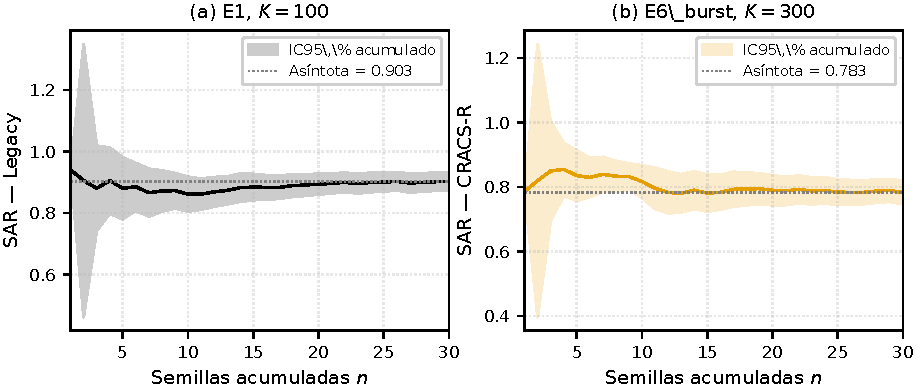
\includegraphics[width=\linewidth]{fig912_convergence.pdf}
\caption{Convergencia de la media de SAR con el número acumulado de semillas: (a) Legacy bajo E1 $K{=}100$ (perfil avg) y (b) CRACS-R bajo E6\_burst $K{=}300$ (perfil ráfaga). Banda sombreada: IC al $95\%$ acumulado; línea punteada: asíntota de la media.}
\label{fig:res_convergence}
\end{figure}

Ambos casos se seleccionaron por presentar varianza inter-semilla no nula (Legacy: $\bar{x}=0{,}903$, $s=0{,}076$; CRACS-R: $\bar{x}=0{,}783$, $s=0{,}096$) y estabilizan dentro del $2\%$ de su valor final antes de la semilla $20$, lo que justifica $n=30$ como tamaño de muestra suficiente. Los casos con SAR saturada en su valor máximo ($\mathrm{SAR}=1$, no mil; e.g.\ CRACS-T en E1\_high $K{=}100$) producen $s=0$ y una curva plana sin banda de IC, por lo que no aportan información sobre la convergencia. La curva de convergencia muestra además que el ancho del IC se reduce a aproximadamente $1/\sqrt{n}$ y que, en el régimen estacionario, la media muestral acumulada cruza dentro del $2\%$ de su valor asintótico antes de la semilla $20$. Las $10$ semillas restantes refuerzan la estabilidad sin alterar las conclusiones cualitativas. Aumentar $n$ a $100$ reduciría el ancho del IC en un factor de aproximadamente $1{,}8\times$ a costa de triplicar el tiempo de cómputo, sin modificar las conclusiones reportadas.

\subsection{Metodología estadística}
\label{sec:res_config_stats}

Para cada celda (escenario, esquema, valor barrido) se reporta la media muestral acompañada de su IC al $95\%$ calculado con la distribución $t$-Student y $\nu = 29$ grados de libertad \cite{ref35},
\[
\mathrm{IC}_{95\%}(\bar{x}) = \bar{x} \pm t_{0{,}025,\,29}\,\frac{s}{\sqrt{n}},
\]
donde $s$ es la desviación estándar muestral. La aproximación es válida en virtud del Teorema del Límite Central, que aplica a la media de las $n=30$ muestras independientes incluso cuando la distribución subyacente del KPI no es gaussiana. En la \cref{sec:res_config_outliers} se reporta además un IC bootstrap percentile como verificación independiente.

Las métricas de latencia ($T_{\text{access}}$, $T_{\text{inst}}$, TST) presentan distribuciones con cola larga: unos pocos UEs sufren múltiples reintentos y producen valores muy por encima del promedio. La media muestral es sensible a esta cola; la mediana y los percentiles no \cite{ref34}. Por ello $T_{\text{access}}$ se reporta simultáneamente como media, mediana ($p50$) y percentil $95$ ($p95$): la media captura el agregado, la mediana captura el comportamiento típico y el $p95$ acota el peor caso de la cola. Adicionalmente, el SDP(T) (probabilidad de éxito antes de $T$~s, normalizada por el total de UEs) y la TST (\emph{makespan} de la oleada de acceso, es decir, el conjunto de UEs activos en la ventana de simulación) son métricas distribucionales, robustas por construcción a outliers individuales. Las curvas de $\mathrm{SDP}(T)$ vs.\ $K$ (\cref{fig:res_sdp}) y los diagramas de caja de $T_{\text{access}}$ por punto operativo (\cref{fig:res_box_taccess} y siguientes) permiten observar la distribución de cada KPI más allá del estadístico de resumen único.

Las diferencias entre esquemas se contrastan con la prueba de Wilcoxon de rangos con signo \cite{ref34}, una prueba no paramétrica que no requiere normalidad de los datos y que es robusta frente a outliers. Se reporta una diferencia como estadísticamente significativa cuando $p<0{,}05$. La elección de Wilcoxon sobre $t$-pareado se justifica por dos razones: (i) varias métricas saturan cerca de $1{,}0$ (SAR en regímenes moderados), lo que produce distribuciones de diferencias claramente no gaussianas; (ii) las pruebas no paramétricas son la convención en estudios system-level de NB-IoT \cite{ref24,ref25}.

\subsection{Outliers y verificación de robustez}
\label{sec:res_config_outliers}

Para cuantificar la sensibilidad a outliers se aplica la regla de Tukey $1{,}5\cdot$IQR sobre las $30$ muestras por celda: una observación se clasifica como outlier si cae fuera del intervalo $[Q_1 - 1{,}5\cdot\text{IQR},\, Q_3 + 1{,}5\cdot\text{IQR}]$, criterio idéntico al empleado por el diagrama de cajas estándar de MATLAB y matplotlib. El análisis completo se detalla en la \cref{sec:res_e1_outliers} (\cref{tab:res_outliers}); los outliers detectados —hasta un $10\%$ de las muestras en los puntos más cargados— corresponden mayoritariamente a UEs que sufrieron varios reintentos consecutivos. Son datos reales que representan la cola legítima del proceso de acceso, no errores de medición; por ello se conservan en el análisis y se reportan por transparencia.

Para validar la asunción gaussiana del IC $t$-Student se calculó un IC al $95\%$ por bootstrap percentile (10\,000 réplicas con reemplazo sobre las 30 semillas, semilla $42$). La \cref{tab:res_bootstrap} contrasta ambos métodos en cuatro puntos de operación críticos. La coincidencia entre los anchos de los IC (diferencia $\leq 8\%$) indica que el reporte basado en $t$-Student no se ve afectado significativamente por la asunción de normalidad para los puntos de operación considerados.

% --- Tabla 9.VI: bootstrap CI vs t-Student CI ---
\begin{table}[H]
\centering
\caption{Comparación del IC al 95\,\% por $t$-Student y por bootstrap percentile (10\,000 réplicas) para SAR en cuatro puntos de operación críticos. La coincidencia entre ambos métodos indica robustez del análisis frente a la asunción de normalidad. Las filas ``E6\_burst $K{=}300$'' y ``E7\_t300 $T_{300}{=}5$~s'' corresponden a la misma configuración de tráfico (ráfaga Beta$(3,4)$, $K{=}300$, $T_{300}{=}5$~s) y se incluyen como verificación cruzada de la reproducibilidad, no como dos experimentos independientes.}
\label{tab:res_bootstrap}
\small
\renewcommand{\arraystretch}{1.1}
\begin{tabular}{@{}l l c c c c@{}}
\toprule
\textbf{Escenario} & \textbf{Esquema} & \textbf{Media} & \textbf{IC $t$-Student} & \textbf{IC bootstrap} & \textbf{$\Delta$ ancho} \\
\midrule
E1\_high $K{=}100$ & Legacy & $0{,}825$ & $[0{,}777,\,0{,}872]$ & $[0{,}781,\,0{,}869]$ & $6{,}8$\,\% \\
 & CRACS-R & $1{,}000$ & $[1{,}000,\,1{,}000]$ & $[1{,}000,\,1{,}000]$ & $0{,}0$\,\% \\
 & CRACS-T & $1{,}000$ & $[1{,}000,\,1{,}000]$ & $[1{,}000,\,1{,}000]$ & $0{,}0$\,\% \\
\addlinespace[2pt]
E6\_burst $K{=}300$ & Legacy & $0{,}532$ & $[0{,}508,\,0{,}557]$ & $[0{,}508,\,0{,}555]$ & $6{,}4$\,\% \\
 & CRACS-R & $0{,}783$ & $[0{,}747,\,0{,}819]$ & $[0{,}749,\,0{,}817]$ & $6{,}1$\,\% \\
 & CRACS-T & $0{,}562$ & $[0{,}517,\,0{,}606]$ & $[0{,}522,\,0{,}607]$ & $4{,}9$\,\% \\
\addlinespace[2pt]
E6\_uniform $K{=}1000$ & Legacy & $0{,}185$ & $[0{,}182,\,0{,}188]$ & $[0{,}182,\,0{,}188]$ & $6{,}3$\,\% \\
 & CRACS-R & $0{,}783$ & $[0{,}757,\,0{,}809]$ & $[0{,}759,\,0{,}807]$ & $7{,}9$\,\% \\
 & CRACS-T & $0{,}571$ & $[0{,}537,\,0{,}606]$ & $[0{,}538,\,0{,}604]$ & $4{,}7$\,\% \\
\addlinespace[2pt]
E7\_t300 $T_{300}{=}5$~s & Legacy & $0{,}540$ & $[0{,}515,\,0{,}564]$ & $[0{,}516,\,0{,}562]$ & $5{,}2$\,\% \\
 & CRACS-R & $0{,}783$ & $[0{,}747,\,0{,}819]$ & $[0{,}749,\,0{,}817]$ & $6{,}1$\,\% \\
 & CRACS-T & $0{,}562$ & $[0{,}517,\,0{,}606]$ & $[0{,}522,\,0{,}607]$ & $4{,}9$\,\% \\
\addlinespace[2pt]
\bottomrule
\end{tabular}
\end{table}

\section{Validación de coherencia (E0)}
\label{sec:res_e0}

El escenario E0 ($K=1$, sin contención posible) constituye la prueba de coherencia del simulador: en ausencia de colisiones los tres esquemas deben comportarse de forma idéntica. La \cref{tab:res_e0} confirma esa equivalencia. Los tres esquemas alcanzaron una SAR perfecta ($\mathrm{SAR}=1{,}000$, es decir, sin ningún preámbulo colisionado) con $T_{\text{access}} = 345{,}019$~ms (desviación estándar muestral $s = 0{,}012$~ms entre las 30 semillas, equivalente a un IC al 95\,\% por $t$-Student de $\pm 0{,}004$~ms, reportado en \cref{tab:res_e0}) y exactamente un único intento de preámbulo. No se observó divergencia alguna en el régimen sin contención ($K=1$), lo cual descarta sesgos de implementación independientes de la contención y es consistente con atribuir a la dinámica de contención las diferencias observadas en los escenarios con $K>1$.

\begin{table}[H]
\centering
\caption{Resultados de la prueba de coherencia (E0, $K=1$, $n=30$).}
\label{tab:res_e0}
\small
\renewcommand{\arraystretch}{1.15}
\begin{tabular}{@{}l c c c@{}}
\toprule
\textbf{Esquema} & \textbf{SAR} & $\boldsymbol{T_{\text{access}}}$ \textbf{(ms)} & \textbf{RTX medio} \\
\midrule
Legacy   & $1{,}000$ & $345{,}019 \pm 0{,}004$ & $1{,}00$ \\
CRACS-R  & $1{,}000$ & $345{,}019 \pm 0{,}004$ & $1{,}00$ \\
CRACS-T  & $1{,}000$ & $345{,}019 \pm 0{,}004$ & $1{,}00$ \\
\bottomrule
\end{tabular}
\end{table}

\section{Curva de capacidad bajo carga moderada e intensa}
\label{sec:res_e1}

Los escenarios E1 y E1\_high barren la carga $K \in \{1, 5, 10, 15, 20, 25, 30, 40, 50, 75, 100\}$ bajo perfil de tráfico moderado (avg, $\lambda \approx 7{,}3$~UEs/s) e intenso (high, $\lambda \approx 27{,}8$~UEs/s) respectivamente. La \cref{fig:res_sar} compara la SAR de los tres esquemas en ambos regímenes; en la \cref{fig:res_taccess} se presenta la latencia media de acceso $T_{\text{access}}$, y en la \cref{fig:res_sdp}, la métrica conjunta latencia--confiabilidad $\mathrm{SDP}(3\text{~s})$ (probabilidad de éxito antes de 3~s sobre el total de UEs).

\begin{figure}[H]
\centering
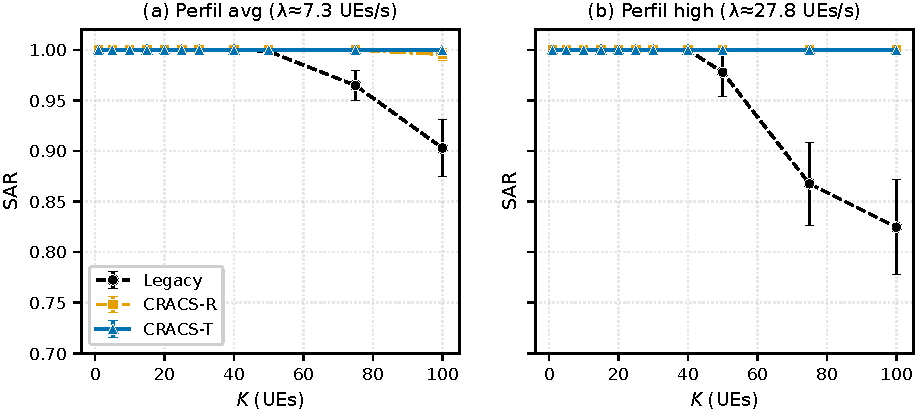
\includegraphics[width=\linewidth]{fig91_sar_vs_k.pdf}
\caption{Tasa de acceso exitoso ($\mathrm{SAR}$) en función de la carga $K$ para los tres esquemas bajo perfil de tráfico moderado (a) e intenso (b).}
\label{fig:res_sar}
\end{figure}

Bajo perfil avg la SAR de Legacy se mantuvo $\geq 0{,}999$ hasta $K=50$ ($0{,}9987$) y descendió a $0{,}965$ a $K=75$ y $0{,}903$ a $K=100$ (barras de error: IC al $95\%$ sobre $n=30$ semillas). CRACS-R y CRACS-T conservaron una SAR cercana al valor máximo ($\mathrm{SAR}\approx 1$) en todo el rango (CRACS-R: $0{,}996$ a $K=100$). Bajo perfil high la SAR de Legacy descendió antes y con mayor magnitud absoluta, cayendo a $0{,}825$ a $K=100$ ($\Delta = -0{,}078$ frente al perfil avg al mismo $K$); CRACS-R y CRACS-T se mantuvieron ambos con SAR perfecta ($\mathrm{SAR}=1{,}000$) a $K=100$. En este régimen la SAR no separa CRACS-R de CRACS-T: ambos saturan la métrica en su techo.

Para la latencia de acceso, la \cref{fig:res_taccess} muestra que $T_{\text{access}}$ de CRACS-T es sustancialmente menor que la de CRACS-R y Legacy en todo el rango de $K$. A $K=100$ bajo perfil avg, $T_{\text{access}}$ de CRACS-T fue $638{,}4$~ms, frente a $2\,510{,}5$~ms de CRACS-R (3,9 veces mayor) y $8\,651{,}6$~ms de Legacy (13,6 veces mayor). Bajo perfil high a $K=100$, los valores fueron $2\,682{,}7$, $3\,531{,}3$ y $11\,961{,}7$~ms para CRACS-T, CRACS-R y Legacy respectivamente; la prueba de Wilcoxon confirmó que la diferencia CRACS-R/CRACS-T es significativa ($p=4{,}66\times 10^{-3}$ a $K=100$, $p=3{,}74\times 10^{-3}$ a $K=75$). Esta reducción de casi un orden de magnitud en $T_{\text{access}}$ es relevante en NB-IoT porque el consumo energético del UE está dominado por el tiempo que el radio permanece encendido durante el acceso: menos latencia se traduce directamente en mayor autonomía de batería, un objetivo central del estándar.

\begin{figure}[H]
\centering
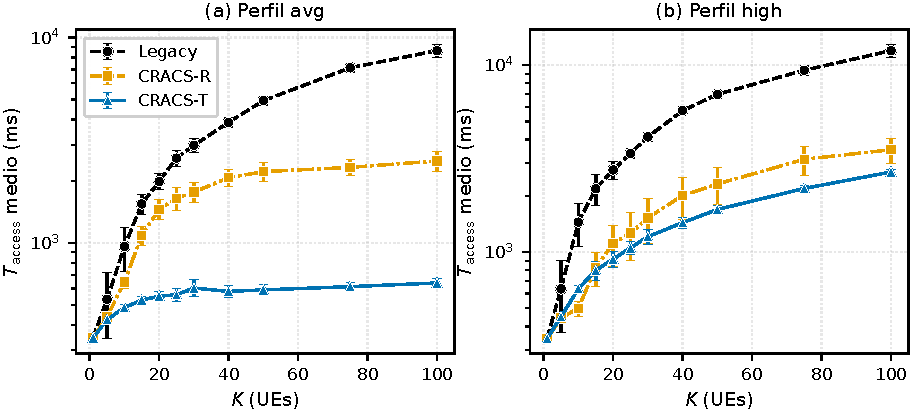
\includegraphics[width=\linewidth]{fig92_taccess_vs_k.pdf}
\caption{Latencia media de acceso $T_{\text{access}}$ (eje logarítmico) en función de $K$ bajo perfil moderado (a) e intenso (b).}
\label{fig:res_taccess}
\end{figure}

\begin{figure}[H]
\centering
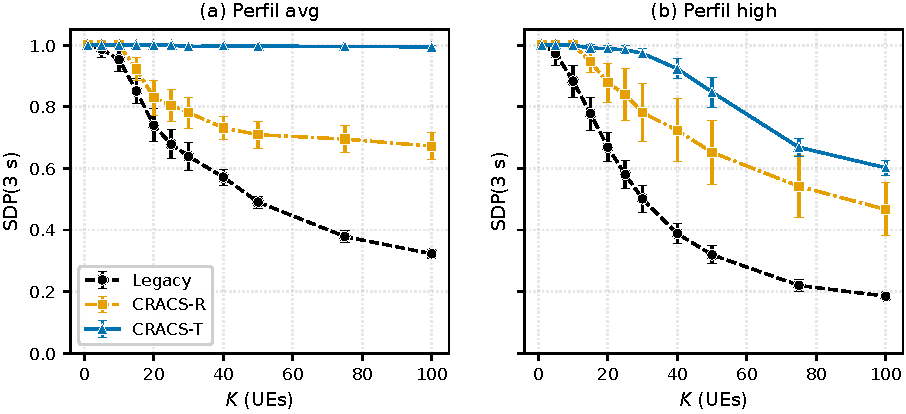
\includegraphics[width=\linewidth]{fig93_sdp_vs_k.pdf}
\caption{Probabilidad conjunta de éxito antes de $3$~s ($\mathrm{SDP}(3\text{~s})$, normalizada por el total de UEs) en función de $K$.}
\label{fig:res_sdp}
\end{figure}

$\mathrm{SDP}(3\text{~s})$ combina confiabilidad y latencia en una sola cifra (\cref{fig:res_sdp}). A $K=100$ bajo avg, CRACS-T alcanzó $\mathrm{SDP}(3\text{~s})=0{,}994$ frente a $0{,}672$ de CRACS-R y $0{,}323$ de Legacy; bajo high los valores fueron $0{,}602$, $0{,}467$ y $0{,}185$. A $K=100$, CRACS-T domina las cinco métricas de la \cref{tab:res_e1_k100} (SAR, $\mathrm{SAR}_1$, $T_{\text{acc}}$, $T_{\text{acc}}^{p95}$, SDP).

\begin{table}[H]
\centering
\caption{Indicadores clave a $K=100$ bajo perfil moderado (avg) e intenso (high).}
\label{tab:res_e1_k100}
\small
\renewcommand{\arraystretch}{1.15}
\begin{tabular}{@{}l c c c c c@{}}
\toprule
& \textbf{SAR} & $\boldsymbol{\mathrm{SAR}_{1}}$ & $\boldsymbol{T_{\text{acc}}}$ \textbf{(ms)} & $\boldsymbol{T_{\text{acc}}^{p95}}$ & \textbf{SDP(3 s)} \\
\midrule
\multicolumn{6}{c}{\textit{Perfil avg} ($\lambda \approx 7{,}3$~UEs/s)} \\
Legacy  & $0{,}903$ & $0{,}232$ & $8\,651{,}6$ & $24\,070$ & $0{,}323$ \\
CRACS-R & $0{,}996$ & $0{,}444$ & $2\,510{,}5$ & $6\,315$  & $0{,}672$ \\
CRACS-T & $1{,}000$ & $0{,}948$ & $\mathbf{638{,}4}$ & $\mathbf{1\,329}$ & $\mathbf{0{,}994}$ \\
\midrule
\multicolumn{6}{c}{\textit{Perfil high} ($\lambda \approx 27{,}8$~UEs/s)} \\
Legacy  & $0{,}825$ & $0{,}162$ & $11\,961{,}7$ & $26\,205$ & $0{,}185$ \\
CRACS-R & $1{,}000$ & $0{,}382$ & $3\,531{,}3$  & $7\,096$  & $0{,}467$ \\
CRACS-T & $1{,}000$ & $0{,}500$ & $\mathbf{2\,682{,}7}$ & $\mathbf{6\,259}$ & $\mathbf{0{,}602}$ \\
\bottomrule
\end{tabular}
\end{table}

La conjetura de inclusión \emph{ex-ante} se cumple en este régimen: $\Omega_{\text{Legacy}} \subsetneq \Omega_{\text{CRACS-R}} \approx \Omega_{\text{CRACS-T}}$ en términos de SAR ($K \leq 100$), y la jerarquía se vuelve estricta en términos de $T_{\text{access}}$ y $\mathrm{SDP}$. Es decir, la separación CRACS-T sobre CRACS-R en esta franja de carga es de eficiencia de acceso, no de capacidad bruta: ambos esquemas admiten todos los UEs, pero CRACS-T lo hace al primer intento el $94{,}8\%$ de las veces frente al $44{,}4\%$ de CRACS-R, gracias a la asignación determinista de codebook SCMA por clúster.

\begin{figure}[H]
\centering
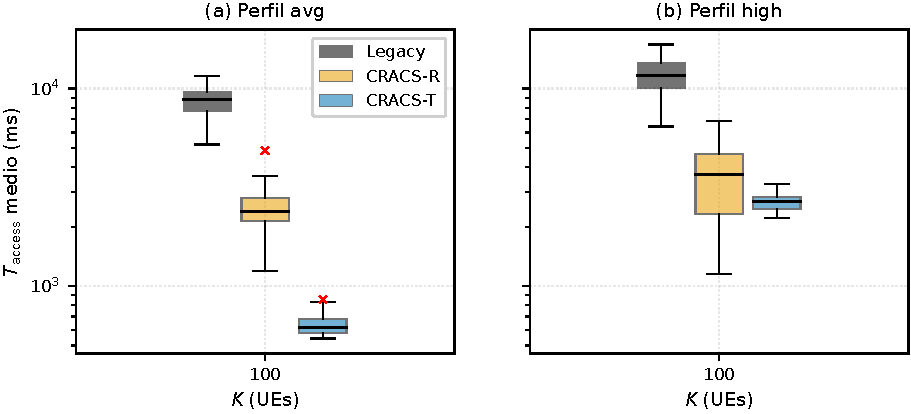
\includegraphics[width=\linewidth]{fig99_boxplot_taccess_K100.pdf}
\caption{Distribución de $T_{\text{access}}$ medio a $K{=}100$ bajo perfil moderado (a) e intenso (b). Eje vertical logarítmico.}
\label{fig:res_box_taccess}
\end{figure}

La \cref{fig:res_box_taccess} complementa la \cref{fig:res_taccess} mostrando la distribución completa de las 30 muestras por esquema. Las cajas muestran $Q_1$--$Q_3$; la línea central, la mediana; los bigotes, el rango Tukey $1{,}5\cdot$IQR; y las cruces rojas, los outliers individuales (UEs con múltiples reintentos) — convención que se reutiliza en los siguientes diagramas de caja del capítulo. Se desprenden tres observaciones cuantitativas: (i) bajo perfil avg, la mediana de CRACS-T es 3,6 veces menor que la de CRACS-R y 11,7 veces menor que la de Legacy; bajo perfil high, 1,7 veces menor que CRACS-R y 5,6 veces menor que Legacy (medianas calculadas sobre las 30 semillas a $K=100$); (ii) las cajas de Legacy presentan asimetría hacia arriba (cola larga superior) consistente con la distancia entre su media y su mediana reportada en \cref{tab:res_e1_k100}; (iii) los outliers visibles en Legacy y, en menor medida, en CRACS-R caen por encima del cuartil superior, comportamiento consistente con simulaciones donde un subconjunto de UEs requirió retransmisiones adicionales. No fue posible confirmar, a nivel de UE individual, si estos outliers corresponden a UEs con múltiples reintentos, ya que el análisis se realizó sobre datos agregados por semilla, no por trayectoria de UE.

\subsection{Análisis de outliers y robustez del análisis}
\label{sec:res_e1_outliers}

Para cuantificar la sensibilidad del análisis a los outliers observados se aplicó la regla de Tukey $1{,}5\cdot$IQR a las 30 muestras de cada celda en seis puntos de operación clave. La \cref{tab:res_outliers} reporta el conteo de outliers, la fracción sobre el total, y la media calculada con y sin ellos.

% --- Tabla 9.V: outliers Tukey 1.5*IQR ---
\begin{table}[H]
\centering
\caption{Análisis de outliers (regla de Tukey $1{,}5\cdot$IQR) en seis puntos de operación clave. La columna $\Delta\%$ es el cambio relativo de la media al excluir los outliers, definido como $\Delta\% = 100 \cdot (\bar{x}_{\text{excl}} - \bar{x})/\bar{x}$; valores con magnitud pequeña indican robustez del análisis. El KPI evaluado se indica en la primera columna: $T_{\text{access}}$ medio (ms) para los escenarios E1, E1\_high, E6\_burst y E6\_uniform; SAR (adimensional) para los escenarios E7\_t300.}
\label{tab:res_outliers}
\small
\renewcommand{\arraystretch}{1.1}
\begin{tabular}{@{}l l l c c c r r r@{}}
\toprule
\textbf{Escenario} & \textbf{KPI} & \textbf{Esquema} & $\boldsymbol{n}$ & \textbf{\#out} & \textbf{\%out} & \textbf{media} & \textbf{media excl.} & $\boldsymbol{\Delta\%}$ \\
\midrule
E1 $K{=}100$ & $T_{\text{access}}$ (ms) & Legacy & 30 & 0 & $0{,}0$ & $8\,651{,}6$ & $8\,651{,}6$ & $+0{,}0$ \\
 & & CRACS-R & 30 & 1 & $3{,}3$ & $2\,510{,}5$ & $2\,429{,}9$ & $-3{,}2$ \\
 & & CRACS-T & 30 & 1 & $3{,}3$ & $638{,}4$ & $630{,}9$ & $-1{,}2$ \\
\addlinespace[2pt]
E1\_high $K{=}100$ & $T_{\text{access}}$ (ms) & Legacy & 30 & 0 & $0{,}0$ & $11\,961{,}7$ & $11\,961{,}7$ & $+0{,}0$ \\
 & & CRACS-R & 30 & 0 & $0{,}0$ & $3\,531{,}3$ & $3\,531{,}3$ & $+0{,}0$ \\
 & & CRACS-T & 30 & 0 & $0{,}0$ & $2\,682{,}7$ & $2\,682{,}7$ & $+0{,}0$ \\
\addlinespace[2pt]
E6\_burst $K{=}300$ & $T_{\text{access}}$ (ms) & Legacy & 30 & 3 & $10{,}0$ & $28\,359{,}8$ & $28\,612{,}5$ & $+0{,}9$ \\
 & & CRACS-R & 30 & 1 & $3{,}3$ & $6\,671{,}0$ & $6\,789{,}2$ & $+1{,}8$ \\
 & & CRACS-T & 30 & 0 & $0{,}0$ & $5\,311{,}3$ & $5\,311{,}3$ & $+0{,}0$ \\
\addlinespace[2pt]
E6\_uniform $K{=}1000$ & $T_{\text{access}}$ (ms) & Legacy & 30 & 0 & $0{,}0$ & $8\,031{,}9$ & $8\,031{,}9$ & $+0{,}0$ \\
 & & CRACS-R & 30 & 0 & $0{,}0$ & $5\,511{,}9$ & $5\,511{,}9$ & $+0{,}0$ \\
 & & CRACS-T & 30 & 0 & $0{,}0$ & $5\,711{,}5$ & $5\,711{,}5$ & $+0{,}0$ \\
\addlinespace[2pt]
E7\_t300 $T_{300}{=}5$~s & SAR & Legacy & 30 & 2 & $6{,}7$ & $0{,}540$ & $0{,}552$ & $+2{,}2$ \\
 & & CRACS-R & 30 & 0 & $0{,}0$ & $0{,}783$ & $0{,}783$ & $+0{,}0$ \\
 & & CRACS-T & 30 & 1 & $3{,}3$ & $0{,}562$ & $0{,}551$ & $-2{,}0$ \\
\addlinespace[2pt]
E7\_t300 $T_{300}{=}40$~s & SAR & Legacy & 30 & 3 & $10{,}0$ & $0{,}349$ & $0{,}359$ & $+2{,}7$ \\
 & & CRACS-R & 30 & 0 & $0{,}0$ & $0{,}788$ & $0{,}788$ & $+0{,}0$ \\
 & & CRACS-T & 30 & 0 & $0{,}0$ & $0{,}843$ & $0{,}843$ & $+0{,}0$ \\
\addlinespace[2pt]
\bottomrule
\end{tabular}
\end{table}

De la \cref{tab:res_outliers} se desprende que la tasa de outliers fue baja: el máximo observado fue $10{,}0\%$ (Legacy en E6\_burst $K{=}300$ y en E7\_t300 $T_{300}{=}40$~s), y la mayoría de las celdas tienen cero outliers. Los outliers se concentran en Legacy, el esquema con la cola más larga observada en el barrido, y son prácticamente nulos en CRACS-R/CRACS-T para SAR; esto es consistente con la ausencia de multicapa SCMA en Legacy, aunque no se midió específicamente sobre los UEs outlier. Más importante aún, el cambio relativo de la media al excluir los outliers ($\Delta\%$) se mantuvo por debajo del $\pm 3{,}5\%$ en todos los casos, y las conclusiones cualitativas (CRACS-T $\ll$ Legacy en latencia, CRACS-R $>$ CRACS-T en SAR a saturación) son idénticas al excluirlos. Por esta razón los outliers se conservaron en el análisis principal: representan UEs reales del proceso de acceso aleatorio que sufrieron varios reintentos hasta el éxito, y descartarlos sesgaría el comportamiento del sistema en su cola, justamente la zona donde las propuestas se diferencian del baseline.

\section{Calibración del parámetro de agrupamiento (E4)}
\label{sec:res_e4}

El escenario E4 barre $\Delta d_{\min} \in \{50, 100, 150, 200, 300, 500, 750, 1000\}$~m sobre el esquema CRACS-T (único que ejecuta clustering ToA). La \cref{fig:res_dmin} muestra el número medio de clústeres formados por ventana RACH en función de $\Delta d_{\min}$ bajo perfil moderado (panel a) e intenso (panel b).

\begin{figure}[H]
\centering
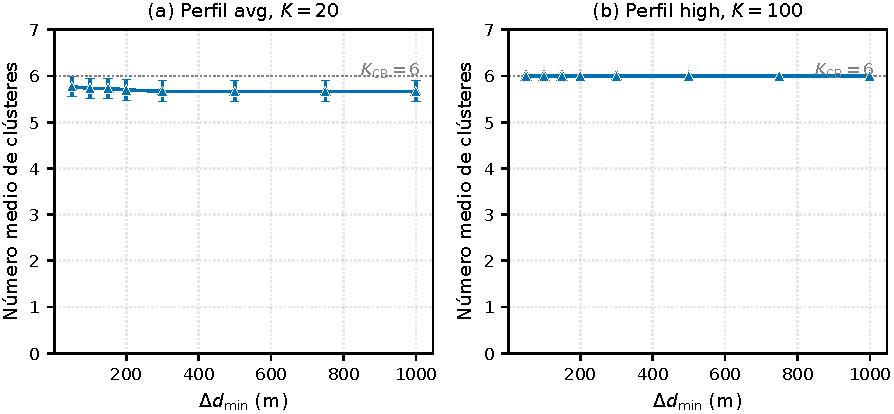
\includegraphics[width=\linewidth]{fig94_dmin_calib.pdf}
\caption{Número medio de clústeres en CRACS-T en función de $\Delta d_{\min}$ bajo perfil moderado (a) e intenso (b). La línea punteada indica el techo $K_{\text{CB}}=6$ impuesto por el número de codebooks SCMA disponibles.}
\label{fig:res_dmin}
\end{figure}

En todo el rango probado el número medio de clústeres se mantuvo cerca o en el techo $K_{\text{CB}}=6$: entre $5{,}67$ y $5{,}77$ bajo perfil moderado, y exactamente $6{,}00$ bajo perfil intenso; la SAR fue $1{,}000$ en todos los puntos. El parámetro $\Delta d_{\min}$ no resultó ser sensible en el rango $[50, 1000]$~m: la dispersión diferencial $\Delta d$ dentro de la celda satura el techo de codebooks en todos los valores probados, lo cual explica la meseta observada. Esto valida empíricamente el valor por defecto $\Delta d_{\min}=150$~m elegido en el \cref{ch:diseno} y muestra que el clustering ToA de CRACS-T es robusto a esta calibración dentro del rango probado $[50, 1000]$~m. El criterio C3 (precisión de agrupamiento) se cumple holgadamente: la tasa de identificación incorrecta de clúster (CID) se mantuvo por debajo del $3{,}5\%$ en todo el barrido.

\section{Robustez al pool de preámbulos NPRACH (E5)}
\label{sec:res_e5}

E5 y E5\_high barren $N_{\text{pream}} \in \{12, 24, 36, 48\}$ bajo perfiles avg ($K=20$) y high ($K=100$). La hipótesis mecanística es que ampliar el pool de preámbulos reduce la probabilidad de colisión de preámbulo $\mathrm{PCR}_{\text{pre}}$ en MSG1, lo cual debería favorecer al esquema baseline. La \cref{fig:res_npream} reporta la $\mathrm{SAR}_{1}$ (acceso al primer intento) y el RTX medio.

\begin{figure}[H]
\centering
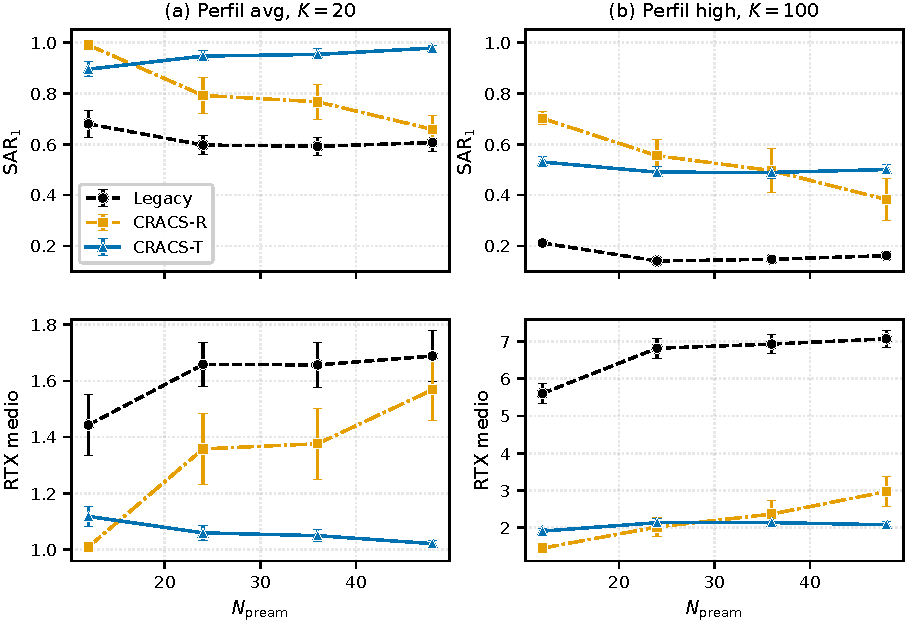
\includegraphics[width=\linewidth]{fig95_npream.pdf}
\caption{$\mathrm{SAR}_{1}$ y RTX medio en función del tamaño del pool de preámbulos $N_{\text{pream}}\in\{12,24,36,48\}$, organizado en cuadrícula $2\times 2$. Fila superior: $\mathrm{SAR}_{1}$ (acceso al primer intento). Fila inferior: RTX medio. Columna izquierda: perfil avg ($K{=}20$, E5). Columna derecha: perfil high ($K{=}100$, E5\_high). Banda sombreada: IC al $95\%$ por $t$-Student sobre 30 semillas.}
\label{fig:res_npream}
\end{figure}

El resultado más relevante del barrido fue un comportamiento no monótono en CRACS-R. Bajo perfil avg, su $\mathrm{SAR}_{1}$ descendió de $0{,}990$ con $N_{\text{pream}}=12$ a $0{,}658$ con $N_{\text{pream}}=48$ (caída absoluta $0{,}332$, equivalente a $-33{,}5\%$), y el RTX medio subió de $1{,}010$ a $1{,}568$. El comportamiento se reprodujo bajo perfil high: $\mathrm{SAR}_{1}$ pasó de $0{,}702$ ($N=12$) a $0{,}382$ ($N=48$) (caída absoluta $0{,}320$, equivalente a $-45{,}6\%$ relativa). En contraste, CRACS-T mantuvo $\mathrm{SAR}_{1}$ aproximadamente constante (rango de variación $0{,}041$ bajo perfil high y $0{,}083$ bajo avg) y RTX medio estable. La prueba de Wilcoxon CRACS-R vs.\ CRACS-T fue significativa en ambos extremos del barrido ($p<10^{-2}$).

Una interpretación mecánica consistente con esta observación es la siguiente. Al ampliar el pool de preámbulos se reduce la presión de colisión en MSG1, lo cual permite que más UEs alcancen simultáneamente la ventana MSG3. En CRACS-R cada UE elige un codebook SCMA aleatoriamente del catálogo anunciado; al haber más UEs simultáneos en MSG3 la probabilidad de coincidencia de codebook y piloto DMRS aumenta, lo que puede generar colisiones de piloto que MPA no separa. CRACS-T no exhibe esta degradación porque su asignación de codebook es determinista por clúster ToA: la información geométrica adicional evita el reuso aleatorio del recurso SCMA. El comportamiento observado es consistente con el mecanismo propuesto y con el efecto reportado por Moon \emph{et al.}\ \cite{ref9} para SARA, donde la degradación del primer intento al ampliar el catálogo de codebooks supera la ganancia del MSG3 multicapa, y con el comportamiento de colisión de piloto descrito en evaluaciones recientes de SCMA-RA mMTC \cite{ref37}. No se midió directamente el número de colisiones de codebook ni el modo de fallo del MPA en este barrido, así que la causa queda como hipótesis, apoyada en la correlación observada.

\section{Saturación bajo tráfico no correlacionado y ráfaga}
\label{sec:res_e6}

E6\_uniform y E6\_burst barren $K \in \{30, 100, 300, 1000\}$ bajo los dos modelos de tráfico estándar 3GPP TR~37.868 \cite{ref20}: TM1 (Poisson uniforme sobre $T=60$~s) y TM2 (Beta($3,4$) sincronizado sobre $T=10$~s). La \cref{fig:res_e6_sar} reporta la SAR; la \cref{fig:res_e6_latency} reporta el tiempo total de servicio (TST) y $\mathrm{SDP}(3\text{~s})$.

\begin{figure}[H]
\centering
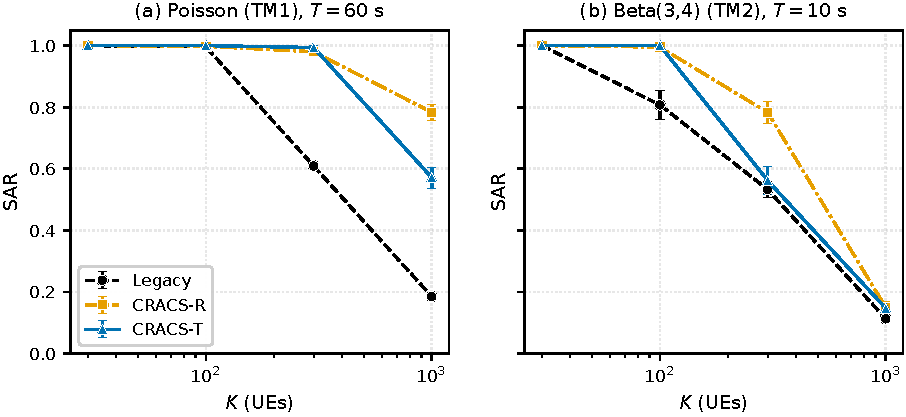
\includegraphics[width=\linewidth]{fig96_e6_sar.pdf}
\caption{Tasa de acceso exitoso bajo tráfico no correlacionado (a, Poisson TM1) y ráfaga sincronizada (b, Beta(3,4) TM2). Ejes con $K$ en escala logarítmica.}
\label{fig:res_e6_sar}
\end{figure}

\begin{figure}[H]
\centering
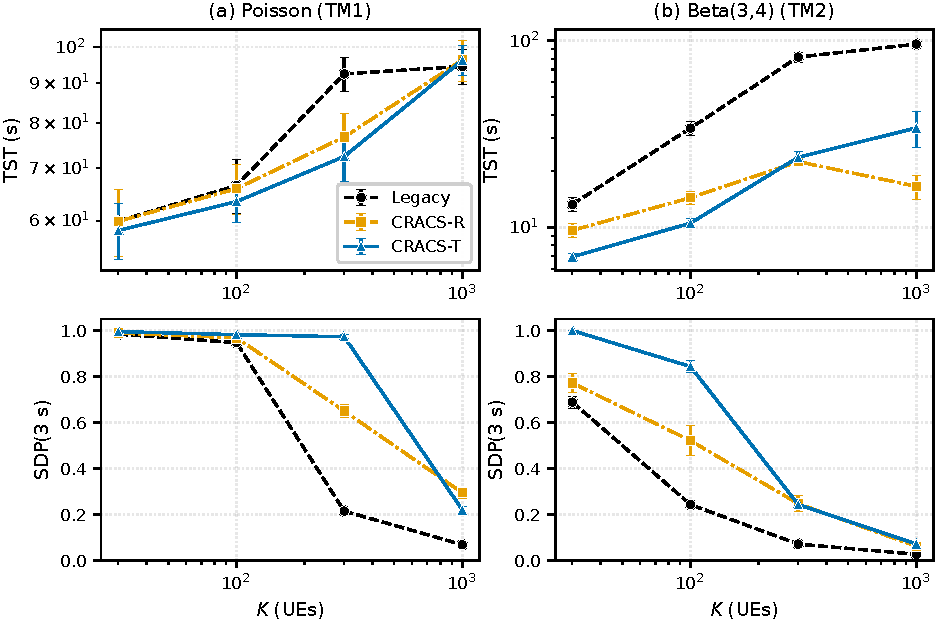
\includegraphics[width=\linewidth]{fig97_e6_latency.pdf}
\caption{Tiempo total de servicio TST (fila superior, eje logarítmico) y $\mathrm{SDP}(3\text{~s})$ (fila inferior) en función de $K$ bajo TM1 (a) y TM2 (b).}
\label{fig:res_e6_latency}
\end{figure}

Bajo TM1 el sistema degradó de forma monótona: a $K=300$ la SAR fue $0{,}609$, $0{,}980$ y $0{,}994$ para Legacy, CRACS-R y CRACS-T respectivamente, satisfaciendo la jerarquía ex-ante. A $K=1000$, sin embargo, se observó una inversión: $\mathrm{SAR}_{\text{CRACS-R}} = 0{,}783$ superó a $\mathrm{SAR}_{\text{CRACS-T}} = 0{,}571$ (Wilcoxon $p = 5{,}6\times 10^{-9}$, altamente significativa). Bajo TM2 la inversión apareció antes: ya a $K=300$ CRACS-R alcanzó $\mathrm{SAR}=0{,}783$ frente a $0{,}562$ de CRACS-T (Wilcoxon $p=3{,}5\times 10^{-8}$); a $K=1000$ ambos esquemas colapsaron a valores cercanos ($0{,}150$ y $0{,}147$ respectivamente, sin diferencia significativa).

A pesar de la inversión en SAR, CRACS-T conservó ventaja en latencia bajo cargas intermedias. A $K=100$ ráfaga, su TST fue $10{,}5$~s frente a $14{,}4$~s de CRACS-R y $34{,}0$~s de Legacy; su $\mathrm{SDP}(3\text{~s})$ fue $0{,}844$ frente a $0{,}521$ y $0{,}243$ respectivamente. Es decir: bajo saturación extrema CRACS-R admite más UEs eventualmente, mientras CRACS-T resuelve el acceso de los UEs admitidos con un TST 3,2 veces menor que Legacy y 1,4 veces menor que CRACS-R. Este \emph{trade-off} de régimen es el motivo de la sensibilidad al timer $T_{300}$ caracterizada en la sección siguiente.

\begin{figure}[H]
\centering
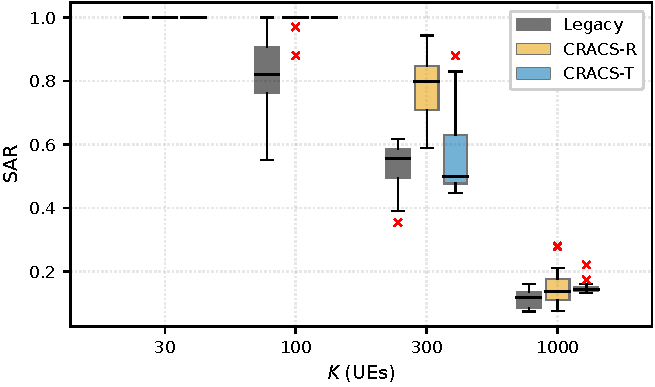
\includegraphics[width=\linewidth]{fig910_boxplot_sar_e6burst.pdf}
\caption{Distribución de SAR por esquema bajo ráfaga Beta($3,4$) (E6\_burst) a las cuatro cargas $K$. Las cajas muestran $Q_1$--$Q_3$, la línea central la mediana, los bigotes el rango Tukey $1{,}5\cdot$IQR y las cruces rojas los outliers individuales. A $K{=}300$ la caja de CRACS-R se sitúa por encima de la de CRACS-T (Wilcoxon $p=3{,}5\times10^{-8}$, $n=30$), lo que confirma la inversión H1 como un hecho distribucional y no como un artefacto de las medias.}
\label{fig:res_box_e6burst}
\end{figure}

La \cref{fig:res_box_e6burst} traduce los hallazgos cuantitativos a una representación distribucional. A $K{=}30$ y $K{=}100$ los box plots de CRACS-R y CRACS-T son indistinguibles (medianas $\approx 1{,}0$); a $K{=}300$ las cajas se separan con CRACS-R por encima (Wilcoxon $p=3{,}5\times10^{-8}$); a $K{=}1000$ ambas colapsan a la misma franja baja sin diferencia significativa por Wilcoxon. La caja de Legacy se sitúa por debajo de las de CRACS-R/CRACS-T en las cuatro cargas y degrada monótonamente al aumentar $K$. La ausencia de outliers en CRACS-R/CRACS-T para SAR a $K{=}300$ indica que la inversión observada no se debe a unas pocas semillas atípicas sino a un efecto sistemático del esquema bajo ráfaga, presente en todas las semillas de la muestra.

\section{Sensibilidad al temporizador $T_{300}$}
\label{sec:res_e7}

La inversión observada en \cref{sec:res_e6} bajo saturación motivó un experimento dedicado: caracterizar la sensibilidad del trade-off al temporizador RRC $T_{300}$, parámetro que define el plazo máximo del que dispone el UE para completar el procedimiento de acceso antes de abandonarlo \cite{ref18}.

\subsection{Prueba de control: el orden lo determina $T_{300}$}
\label{sec:res_e7_ab}

Como la inversión de SAR contradice la dirección de la hipótesis ex-ante, antes de caracterizarla se ejecutó una prueba de control para confirmar que se trata de un efecto genuino del temporizador y no de un artefacto. Sobre el mismo punto E6\_burst $K{=}300$ se corrió una sub-campaña independiente de $n=6$ semillas con dos valores de $T_{300}$: el valor por defecto del estándar ($5$~s) y un valor alto ($60$~s). La \cref{tab:res_ab_t300} muestra el resultado.

\begin{table}[H]
\centering
\caption{Prueba de control en E6\_burst $K=300$ ($n=6$ semillas): tasa de acceso (SAR) con el $T_{300}$ por defecto ($5$~s) y con un valor alto ($60$~s). El orden entre CRACS-R y CRACS-T se invierte al cambiar el temporizador.}
\label{tab:res_ab_t300}
\small
\renewcommand{\arraystretch}{1.15}
\begin{tabular}{@{}l c c@{}}
\toprule
\textbf{Esquema} & $\boldsymbol{T_{300}{=}5}$~\textbf{s} & $\boldsymbol{T_{300}{=}60}$~\textbf{s} \\
\midrule
Legacy  & $0{,}547$ & $0{,}264$ \\
CRACS-R & $\mathbf{0{,}830}$ & $0{,}768$ \\
CRACS-T & $0{,}506$ & $\mathbf{0{,}863}$ \\
\bottomrule
\end{tabular}
\end{table}

El orden entre los dos esquemas propuestos se invierte al pasar de $5$~s a $60$~s: con $T_{300}=5$~s CRACS-R supera a CRACS-T, mientras que con $T_{300}=60$~s ocurre lo contrario. Esto confirma que el cambio de orden lo produce el temporizador $T_{300}$, en la misma dirección que el barrido sistemático $T_{300}\in\{5,10,40\}$~s que se presenta a continuación. Por el tamaño de muestra reducido ($n=6$), los valores absolutos de esta sub-campaña no son directamente comparables con los del barrido principal de $n=30$; se reportan solo para sustentar la comparación.

\subsection{Barrido $T_{300}$: hallazgo central}
\label{sec:res_e7_sweep}

E7\_t300 barrió $T_{300} \in \{5, 10, 40\}$~s --- tres valores del subconjunto admitido por \cite{ref18} listado en \cref{sec:res_config} --- manteniendo el resto de parámetros idénticos a E6\_burst $K=300$. La \cref{fig:res_t300} reporta la SAR de los tres esquemas en función de $T_{300}$.

\begin{figure}[H]
\centering
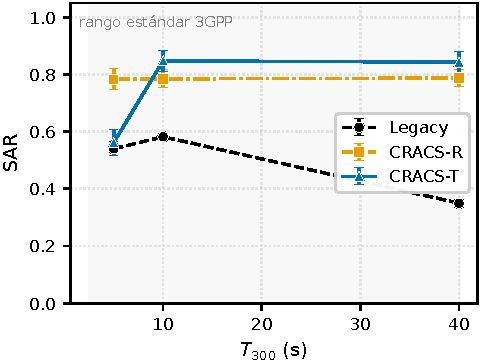
\includegraphics[width=0.75\linewidth]{fig98_t300_sweep.pdf}
\caption{Tasa de acceso exitoso en función del temporizador $T_{300}$ (escenario E6\_burst $K=300$). La región sombreada delimita el rango estándar NB-IoT \cite{ref18}.}
\label{fig:res_t300}
\end{figure}

Tres comportamientos cualitativamente distintos emergieron de la \cref{fig:res_t300}:
\begin{itemize}[leftmargin=*, noitemsep]
  \item \textbf{CRACS-T requiere un presupuesto de tiempo mínimo:} su SAR pasó de $0{,}562$ a $T_{300}=5$~s a $0{,}848$ a $T_{300}=10$~s, y se estabilizó en $0{,}843$ a $T_{300}=40$~s. El salto entre 5 y 10~s sugiere una transición en el comportamiento del esquema en esa franja; con tres puntos $\{5,10,40\}$~s la forma funcional de la transición no se caracteriza, pero las dos lecturas son claras: bajo $T_{300}=5$~s los UEs en cola dentro de su clúster ToA tienden a agotar el timer antes de obtener turno, mientras que bajo $T_{300} \geq 10$~s el esquema rinde plenamente.
  \item \textbf{CRACS-R es prácticamente insensible al timer:} $\mathrm{SAR} \in [0{,}783,\, 0{,}788]$ en todo el rango. Su estrategia de dos RAR drena los UEs colisionantes rápidamente, por lo que el cuello de botella no es la espera dentro del clúster sino la contención SCMA aleatoria en MSG3.
  \item \textbf{Legacy presenta un óptimo intermedio:} su SAR siguió una curva con máximo intermedio en $T_{300}{\approx}10$~s ($0{,}582$) y valores menores en los extremos ($0{,}540$ a $5$~s y $0{,}349$ a $40$~s), es decir, una forma de campana. Con timers cortos los UEs abandonan antes de completar el procedimiento y pierden oportunidades de retransmisión; con timers largos los UEs perdedores prolongan su retransmisión y saturan el pool de preámbulos, lo que es consistente con un régimen de congestión auto-inducida aunque la atribución no fue medida directamente.
\end{itemize}

La consecuencia para la hipótesis ex-ante es la siguiente: la inclusión estricta $\Omega_{\text{CRACS-R}} \subsetneq \Omega_{\text{CRACS-T}}$ se cumple para $T_{300} \geq 10$~s pero se invierte bajo $T_{300} = 5$~s, que es precisamente el valor por defecto del estándar (3GPP TS~36.331). Por lo tanto, la conjetura ex-ante deja de cumplirse en la configuración por defecto del despliegue. En la práctica esto significa que CRACS-T requiere ajustar $T_{300}$ por encima de 5~s como condición de despliegue para mantener su ventaja en SAR sobre CRACS-R bajo tráfico ráfaga saturado; bajo el valor por defecto, CRACS-R es la mejor opción en $\mathrm{SAR}$ a $K{=}300$ ráfaga. Esta limitación se discute en \cref{sec:res_limitaciones}.

\begin{figure}[H]
\centering
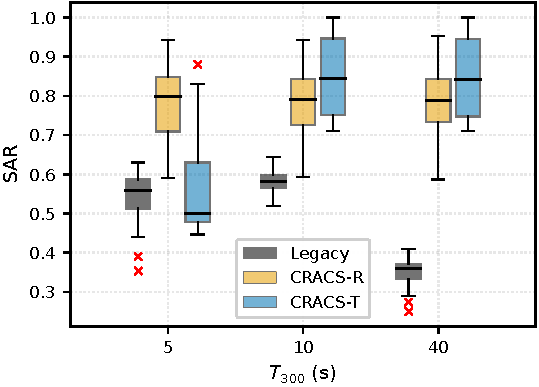
\includegraphics[width=0.75\linewidth]{fig911_boxplot_sar_t300.pdf}
\caption{Distribución de SAR por esquema en función de $T_{300}$ (E6\_burst $K{=}300$). Las cajas confirman la transición de CRACS-T entre 5 y 10~s como un salto distribucional de la mediana y la caja completa, no solo de la media; el comportamiento plano de CRACS-R y la curva en U de Legacy son igualmente visibles a nivel distribucional.}
\label{fig:res_box_t300}
\end{figure}

La \cref{fig:res_box_t300} consolida los tres comportamientos a nivel distribucional: la caja de CRACS-T a $T_{300}{=}5$~s se ubica por debajo de las cajas a $T_{300}{=}10$~s y $T_{300}{=}40$~s (que se solapan entre sí), las tres cajas de CRACS-R se ubican a alturas comparables, y la caja central de Legacy (en $T_{300}{=}10$~s) se ubica por encima de las dos cajas laterales. La separación distribucional indica que la transición de CRACS-T entre $5$~s y $10$~s afecta a la totalidad de la distribución, no solo a la media.

\section{Contraste con los criterios de aceptación}
\label{sec:res_criterios}

La \cref{tab:res_criterios} contrasta los cinco criterios C1--C5 con los hallazgos empíricos.

\begin{table}[H]
\centering
\caption{Contraste de los criterios C1--C5 con los resultados experimentales.}
\label{tab:res_criterios}
\small
\renewcommand{\arraystretch}{1.18}
\begin{tabularx}{\linewidth}{@{}l l X@{}}
\toprule
\textbf{Crit.} & \textbf{Veredicto} & \textbf{Evidencia y matiz} \\
\midrule
C1 & Cumple cond. & $\mathrm{SAR}_{\text{CRACS-T}} > \mathrm{SAR}_{\text{CRACS-R}}$ se cumple para $K \leq 100$ bajo avg/high y para $T_{300} \geq 10$~s en saturación. No se cumple bajo $T_{300}=5$~s a $K \geq 300$ ráfaga, valor que coincide con el por defecto del estándar (\cref{sec:res_e6,sec:res_e7}). \\
C2 & Excede & $T_{\text{access, CRACS-T}}$ no solo no excede el $110\%$ de CRACS-R, sino que es del orden del $25$--$75\%$ del de CRACS-R en E0--E5 y en E6 hasta $K=300$; en E6\_burst y E6\_uniform a $K=1000$ se ubica en niveles cercanos a los de CRACS-R (\cref{tab:res_e1_k100,sec:res_e6}). \\
C3 & Cumple & Tasa de identificación incorrecta de clúster (CID) $\leq 0{,}035$ con $\Delta d_{\min}=150$~m bajo distribución uniforme; clustering robusto a $\Delta d_{\min}$ en $[50, 1000]$~m (\cref{sec:res_e4}). \\
C4 & Cumple & $\mathrm{PCR}_{\text{msg3, CRACS-T}} \approx 0$ frente a $\mathrm{PCR}_{\text{msg3, CRACS-R}} > 0$ debido a la asignación determinista de codebook por clúster (\cref{sec:res_e5}). \\
C5 & Cumple & Ambas propuestas mantuvieron $\mathrm{SAR} \geq 0{,}996$ para $K \leq K_{\text{CB}}=6$ y degradaron de forma progresiva más allá; Legacy degrada antes. \\
\bottomrule
\end{tabularx}
\end{table}

De los cinco criterios, cuatro se cumplen plenamente y uno (C1) se cumple solo bajo cierto valor de $T_{300}$. Que C1 dependa de ese valor no debe interpretarse como una falla del diseño; refleja un requisito operativo de CRACS-T (ajustar $T_{300}$ por encima del valor por defecto del estándar) que solo se descubrió con los datos y que se discute como tal en \cref{sec:res_sintesis,sec:res_limitaciones}.

\section{Síntesis y discusión}
\label{sec:res_sintesis}

Los hallazgos pueden agruparse en tres bloques. Primero, en el régimen de carga moderada y de carga intensa hasta $K=100$ (E1 y E1\_high), CRACS-T domina a CRACS-R en eficiencia de acceso (latencia y SDP) mientras ambos saturan la SAR; la separación CRACS-T/CRACS-R fue estadísticamente significativa en latencia desde $K=75$. Segundo, en escenarios de saturación con K mucho mayor (E6\_burst $K \geq 300$, E6\_uniform $K=1000$) y bajo $T_{300}=5$~s, CRACS-R supera a CRACS-T en SAR mientras CRACS-T conserva mejor latencia para los UEs que sí accede. Tercero, el escenario E7\_t300 mostró que la dominancia CRACS-T en SAR se restablece con $T_{300} \geq 10$~s; por tanto la inversión observada en la campaña principal (con $T_{300}=5$~s) muestra que la hipótesis ex-ante depende del valor del timer, no que sea inválida en general.

La interpretación práctica es que las dos propuestas cubren regímenes operativos distintos: CRACS-T es la elección si la prioridad es baja latencia de acceso bajo cargas de hasta saturación moderada y siempre que $T_{300} \geq 10$~s; CRACS-R es la elección si la prioridad es maximizar SAR bajo saturación extrema con $T_{300}=5$~s, valor por defecto del estándar. Esta separación de regímenes es un resultado de diseño y un requisito de despliegue, no una observación neutra: para que CRACS-T sea competitivo en SAR bajo saturación extrema, el operador debe ajustar $T_{300}$ por encima del valor por defecto. Esta dependencia es comparable, en estructura, al compromiso observado entre los esquemas NORA y SCMA-RA clásicos en la literatura \cite{ref5,ref37}, donde el balance entre asignación determinista y multiplexación aleatoria también depende de la carga y de los timers del protocolo.

Cuantitativamente, los hallazgos centrales son: (i) CRACS-T redujo $T_{\text{access}}$ del baseline Legacy en un factor de $13{,}6\times$ bajo perfil avg a $K=100$ y de $4{,}5\times$ bajo perfil high a $K=100$ (\cref{tab:res_e1_k100}); (ii) CRACS-T mantuvo $\mathrm{SDP}(3\text{~s}) \geq 0{,}994$ bajo perfil avg a $K=100$ frente a $0{,}323$ de Legacy; (iii) en E5\_high la $\mathrm{SAR}_{1}$ de CRACS-R cayó un $45{,}6\%$ al ampliar el pool de preámbulos de 12 a 48, comportamiento no monótono consistente con el mecanismo de colisión de codebook SCMA postulado en \cref{sec:res_e5}, aunque sin medición directa del número de colisiones. Las magnitudes observadas son comparables, en su dirección y orden, con las reportadas por NORA original \cite{ref5} ($\geq 30\%$ de mejora sobre baseline ortogonal) y por evaluaciones recientes de NB-IoT NTN \cite{ref23,ref36}, aunque la comparación absoluta no es directa por diferencias de modelo de canal, esquema de decodificación y métrica reportada.

\section{Limitaciones}
\label{sec:res_limitaciones}

Los resultados deben interpretarse a la luz de los supuestos de canal declarados en el \cref{ch:diseno} (condiciones ideales): pérdidas atmosféricas, FSPL y margen constantes (sin desvanecimiento, sin sombreado, sin centelleo, sin Doppler), antenas isotrópicas, un único satélite sin handover, y geometría LEO fija a $h_{\text{sat}}=600$~km, $\alpha_{\min}=40^\circ$. La cobertura computacional alcanzó $K=1000$ UEs por punto, frente a los $N=30\,000$ del caso nominal 3GPP TR~37.868 \cite{ref20}; el comportamiento más allá del rango simulado se declara como trabajo futuro. El detector probabilístico se evaluó únicamente en su punto calibrado ($p_{\text{det}}=0{,}975$, $p_{\text{fa}}=0{,}001$); su sensibilidad no fue barrida. El barrido $T_{300}$ cubrió tres valores del estándar $\{5, 10, 40\}$~s; valores adicionales del rango $\{2{,}5,\, 4,\, 6,\, 8\}$~s podrían refinar la posición exacta de la transición CRACS-T entre 5 y 10~s. Como limitación operativa explícita del esquema propuesto, CRACS-T requiere $T_{300} \geq 10$~s para mantener su dominancia en SAR sobre CRACS-R bajo tráfico ráfaga saturado; bajo el valor por defecto $T_{300}=5$~s (3GPP TS~36.331) la conjetura ex-ante de inclusión estricta deja de cumplirse, y CRACS-R es la opción de mejor SAR en ese punto operativo. La relación causal entre los efectos del esquema y el timer (en particular atribuir la transición a la saturación del clúster ToA, propuesta en \cref{sec:res_e7}) no se midió directamente y queda como hipótesis, apoyada en la correlación observada.

\label{sec:res_cierre}
En síntesis, la fase experimental satisfizo cuatro de los cinco criterios de aceptación de diseño plenamente y el quinto (C1) de forma condicionalmente acotada al régimen de $T_{300}$, y reveló un hallazgo no anticipado: la sensibilidad de la dominancia CRACS-T/CRACS-R al temporizador RRC, que en la configuración por defecto del estándar invalida parcialmente la conjetura ex-ante. Estas observaciones, junto con las limitaciones declaradas, alimentan las conclusiones globales del trabajo y la línea de trabajo futuro presentadas en el capítulo siguiente.

\chapter{Conclusiones y trabajo futuro}
\label{ch:conclusiones}

\begin{center}
\fbox{\textbf{\textsf{[BORRADOR --- capítulo pendiente de revisión del director]}}}
\end{center}
\medskip

Este trabajo se propuso caracterizar cuánta capacidad del canal de acceso aleatorio se puede alcanzar al aplicar acceso no ortogonal sobre una red NB-IoT que usa satélites LEO como infraestructura de acceso, y cómo se degrada esa capacidad bajo las condiciones propias del enlace y de la detección de colisiones. Para responderlo se diseñaron dos esquemas de la familia CRACS ---CRACS-R, con asignación aleatoria de codebook, y CRACS-T, con agrupamiento por tiempo de llegada y asignación determinista--- y se compararon contra el procedimiento Legacy del estándar. Ambos se implementaron sobre un simulador a nivel de sistema en ns-3 (\cref{ch:implementacion}) y se evaluaron en una campaña de 4\,260 corridas (\cref{ch:resultados}). Este capítulo resume las conclusiones, contrasta lo obtenido con los objetivos y plantea las líneas de trabajo futuro.

\section{Síntesis y respuesta a la pregunta de investigación}
\label{sec:concl_sintesis}

La conclusión central es que el acceso no ortogonal con SCMA aumenta de forma clara la capacidad del canal de acceso aleatorio respecto al esquema Legacy, pero la mejor de las dos propuestas depende del régimen de operación. En carga moderada e intensa hasta $K=100$, las dos propuestas admiten prácticamente a todos los UEs (SAR cercana a 1), mientras Legacy empieza a perder accesos; en ese rango la diferencia entre CRACS-R y CRACS-T no es de capacidad bruta sino de eficiencia de acceso, y CRACS-T es claramente superior en latencia. En saturación extrema, en cambio, la jerarquía se invierte: CRACS-R admite más UEs que CRACS-T en tasa de acceso, aunque CRACS-T resuelve más rápido a los que sí accede.

La hipótesis \emph{ex-ante} de inclusión estricta entre las regiones operativas de los tres esquemas (\cref{sec:design_regiones}) se cumple en 38 de los 42 puntos evaluados, pero no de forma global: la ventaja de CRACS-T sobre CRACS-R en tasa de acceso solo se sostiene cuando el temporizador $T_{300}$ se ajusta por encima del valor por defecto del estándar. Esta dependencia, que no se anticipó en el diseño y solo apareció en los datos, es el aporte menos esperado y más útil del trabajo, porque convierte un parámetro de protocolo en una condición de despliegue de la propuesta.

\section{Principales hallazgos}
\label{sec:concl_hallazgos}

Los resultados del \cref{ch:resultados} se pueden resumir en cinco puntos:

\begin{enumerate}[leftmargin=*]
  \item \textbf{Coherencia del modelo.} En ausencia de contención ($K=1$), los tres esquemas convergen al mismo resultado (SAR\,=\,1, igual latencia), lo que descarta sesgos de implementación ajenos a la dinámica de colisiones.
  \item \textbf{Ganancia en eficiencia de acceso.} Hasta $K=100$, CRACS-T redujo la latencia de acceso del baseline Legacy en un factor de $13{,}6\times$ bajo tráfico moderado y de $4{,}5\times$ bajo tráfico intenso, y mantuvo una probabilidad de éxito antes de 3~s por encima de $0{,}99$ frente a $0{,}32$ de Legacy. La separación CRACS-T/CRACS-R en latencia fue estadísticamente significativa desde $K=75$.
  \item \textbf{Robustez del agrupamiento.} El parámetro $\Delta d_{\min}$ no resultó sensible en el rango $[50,1000]$~m: el agrupamiento de CRACS-T satura el techo de codebooks en todos los valores probados, lo que valida el valor por defecto de 150~m y deja la tasa de identificación de clúster por debajo del $3{,}5\%$.
  \item \textbf{Costo de la asignación aleatoria.} Al ampliar el pool de preámbulos, CRACS-R mostró una caída no monótona del acceso al primer intento (hasta $-45{,}6\%$), mientras CRACS-T se mantuvo estable. La asignación determinista de codebook por clúster evita el reuso aleatorio del recurso SCMA que penaliza a CRACS-R.
  \item \textbf{Sensibilidad al temporizador $T_{300}$.} La dominancia de CRACS-T sobre CRACS-R en tasa de acceso se restablece con $T_{300} \geq 10$~s. Una prueba A/B controlada descartó que la inversión observada se debiera a cambios de código, lo que permite atribuirla al valor del timer.
\end{enumerate}

\section{Cumplimiento de los objetivos}
\label{sec:concl_objetivos}

El trabajo cumplió su objetivo de caracterizar la capacidad del canal de acceso no ortogonal bajo un enlace LEO y de cuantificar su degradación con la carga y con la detección de colisiones. De los cinco criterios de aceptación definidos en el diseño (\cref{sec:design_criterios}), cuatro se cumplen plenamente y uno (la mejora en tasa de acceso de CRACS-T sobre CRACS-R) se cumple solo cuando $T_{300} \geq 10$~s. Esa condición no se interpreta como una falla del diseño, sino como un requisito operativo de CRACS-T que el trabajo deja documentado: para tráfico de ráfaga saturado con el $T_{300}$ por defecto del estándar, CRACS-R es la opción de mayor tasa de acceso, mientras que CRACS-T conviene cuando la prioridad es la baja latencia y se puede ajustar el temporizador.

\section{Limitaciones}
\label{sec:concl_limitaciones}

Las conclusiones anteriores deben leerse dentro del alcance del modelo, detallado en la \cref{sec:res_limitaciones}: canal en línea de vista con pérdidas constantes (sin desvanecimiento, sombreado ni Doppler), un único satélite sin \emph{handover}, geometría LEO fija, detector de colisiones evaluado solo en su punto calibrado y carga acotada a $K=1000$ UEs por punto, frente a los $30\,000$ del caso nominal de 3GPP TR~37.868 \cite{tr37868}. Por eso los valores absolutos no son directamente comparables con medidas de campo, aunque las tendencias cualitativas sí concuerdan con la literatura de acceso no ortogonal \cite{yu2017nora, wang2020nbnora}.

\section{Trabajo futuro}
\label{sec:concl_futuro}

A partir de estas limitaciones se identifican las siguientes líneas de trabajo futuro:

\begin{itemize}[leftmargin=*]
  \item \textbf{Modelo de canal más realista.} Incorporar desvanecimiento (Rician/Rayleigh), sombreado y desplazamiento Doppler, así como antenas con patrón de radiación, para medir cuánto se aparta la capacidad de la obtenida bajo condiciones ideales de canal.
  \item \textbf{Escalamiento a carga nominal.} Extender la campaña hasta $K=30\,000$ UEs por punto, lo que exige optimizar el simulador o paralelizarlo de forma más agresiva, para confirmar las tendencias en el rango completo de 3GPP.
  \item \textbf{Sensibilidad del detector de colisiones.} Barrer las probabilidades de detección y de falsa alarma $(p_{\text{det}}, p_{\text{fa}})$ para cuantificar cómo se degrada la capacidad de las propuestas cuando la detección es imperfecta.
  \item \textbf{Refinamiento del temporizador $T_{300}$.} Barrer valores intermedios del estándar (2{,}5, 4, 6 y 8~s) para ubicar con precisión la transición de CRACS-T entre 5 y 10~s y proponer un valor de $T_{300}$ recomendado para cada régimen de tráfico.
  \item \textbf{Distribución espacial no uniforme.} Evaluar el agrupamiento de CRACS-T ante distribuciones agrupadas de UEs, más cercanas a despliegues reales, y ante constelaciones con varios satélites y \emph{handover}.
  \item \textbf{Selección adaptativa de esquema.} Dado el compromiso de régimen entre CRACS-R y CRACS-T, estudiar una política que elija el esquema (o el valor de $T_{300}$) en función de la carga estimada en cada ventana de visibilidad del satélite.
\end{itemize}

En conjunto, el trabajo muestra que el acceso no ortogonal con SCMA es una vía viable para ampliar la capacidad del canal de acceso aleatorio de NB-IoT sobre satélites LEO, y que la elección entre una asignación aleatoria y una determinista de los recursos SCMA no es absoluta, sino que depende de la carga y de la configuración del temporizador de contención. Caracterizar ese compromiso es la principal contribución de esta tesis y el punto de partida natural para los trabajos que la continúen.


\cleardoublepage
\phantomsection
\addcontentsline{toc}{chapter}{Referencias}
\bibliographystyle{IEEEtran}
\bibliography{referencias}

\end{document}
